% Copyright 2021 Politecnico di Milano, Italy. Inc. All rights reserved

\documentclass{PoliMi_MasterThesis}

% === Packages and configurations ===
% Configurations
\usepackage{parskip} % For paragraph layout
\usepackage{setspace} % For using single or double spacing
\usepackage{emptypage} % To insert empty pages
\setlength\parindent{0pt} % Indentation
\raggedbottom % Do not stretch empty space to fill the page

% Titles
\usepackage{titlesec}
% \titlespacing{\section}{left spacing}{before spacing}{after spacing}
\titlespacing{\section}{0pt}{3.3ex}{2ex}
\titlespacing{\subsection}{0pt}{3.3ex}{1.65ex}
\titlespacing{\subsubsection}{0pt}{3.3ex}{1ex}
\usepackage{color}

% Language and fonts
\usepackage[english]{babel} % The document is in English  
\usepackage[utf8]{inputenc} % UTF8 encoding
\usepackage[T1]{fontenc} % Font encoding
\usepackage[11pt]{moresize} % Big fonts

% Images
\usepackage{graphicx} % For images
\graphicspath{{./Images/}} % Directory of the images
\usepackage{transparent} % Enables transparent images
\usepackage{eso-pic} % For the background picture on the title page
\usepackage{subfig} % Numbered and caption sub-figures using \subfloat.
\usepackage{tikz} % A package for high-quality hand-made figures.
\usetikzlibrary{}
\usepackage{xcolor} % Coloured captions
\usepackage{amsthm,thmtools,xcolor} % Coloured "Theorem"
\usepackage{float}
\usepackage[font=small]{caption} % To make captions small
\usepackage{eso-pic} % Background pictures for each page
\newcommand*\triangleLogo{
	\clearpage
	\thispagestyle{empty}
	\newpage
	\begin{figure}
		\centering
		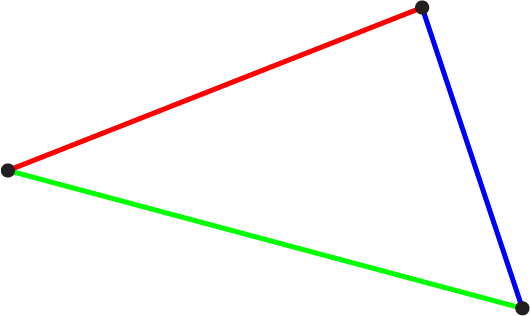
\includegraphics[width=\textwidth]{Images/triangle_logo_thin.png} 
	\end{figure}
}

% Math
\usepackage{amsmath}
\usepackage{amsthm}
\usepackage{amssymb}
\usepackage{amsfonts}
\usepackage{bm}
\usepackage[overload]{empheq} % For braced-style systems of equations.
\usepackage{fix-cm} % To override original LaTeX restrictions on sizes

% Tables
\usepackage{tabularx}
\usepackage{longtable} % Tables that can span several pages
\usepackage{colortbl}

% Algorithms
\usepackage{algorithm}
\usepackage{algorithmicx}
\usepackage{algpseudocodex}
\newcommand*\Let[2]{\State #1 $\gets$ #2}
\newcommand*\Class[1]{\State $\textbf{class} \;$ #1}
\newcommand*\Member[2]{\State $\qquad$ #1 $:$ #2}
\newcommand*\AAnd{\textbf{ and }}
\newcommand*\AOr{\textbf{ or }}
\newcommand*\ANot{\textbf{not }}

% Bibliography
\usepackage[colorlinks=true,linkcolor=black,anchorcolor=black,citecolor=black,filecolor=black,menucolor=black,runcolor=black,urlcolor=black]{hyperref} % Adds clickable links at references
\usepackage{cleveref}
\usepackage[square, numbers, sort&compress]{natbib} % Square brackets, citing references with numbers, citations sorted by appearance in the text and compressed
\bibliographystyle{abbrvnat} % You may use a different style adapted to your field

% Other packages
\usepackage{pdfpages} % To include a pdf file
\usepackage{afterpage}
\usepackage{fancyhdr} % For the headers
\fancyhf{}

% Input of configuration file. Do not change config.tex file unless you really know what you are doing. 
% Set the geometric layout of the document
\usepackage{geometry}
\geometry{
  top=3cm,
  left = 1.5cm,
  right = 1.5cm,
  bottom=2cm,
  headheight= 2cm,
  headsep= 0cm,
}
\raggedbottom 

% Create color bluePoli (-> manuale grafica coordinata:  https://www.polimi.it/fileadmin/user_upload/il_Politecnico/grafica-coordinata/2015_05_11_46xy_manuale_grafica_coordinata.pdf)
\definecolor{bluePoli}{cmyk}{0.4,0.1,0,0.4}

% Custom theorem environments
\declaretheoremstyle[
  headfont=\color{bluePoli}\normalfont\bfseries,
  bodyfont=\color{black}\normalfont\itshape,
]{colored}

\captionsetup[figure]{labelfont={color=bluePoli}} % Set colour of the captions
\captionsetup[table]{labelfont={color=bluePoli}} % Set colour of the captions
\captionsetup[algorithm]{labelfont={color=bluePoli}} % Set colour of the captions

\theoremstyle{colored}
\newtheorem{theorem}{Theorem}[section]
\newtheorem{proposition}{Proposition}[section]

% Enhances the features of the standard "table" and "tabular" environments.
\newcommand\T{\rule{0pt}{2.6ex}}
\newcommand\B{\rule[-1.2ex]{0pt}{0pt}}

% Algorithm description
\newcounter{algsubstate}
\renewcommand{\thealgsubstate}{\alph{algsubstate}}
\newenvironment{algsubstates}{
    \setcounter{algsubstate}{0}%
    \renewcommand{\STATE}{%
    \stepcounter{algsubstate}%
    \Statex {\small\thealgsubstate:}\space}
    }{}
    
% Custom theorem environment
\newcolumntype{L}[1]{>{\raggedright\let\newline\\\arraybackslash\hspace{0pt}}m{#1}}
\newcolumntype{C}[1]{>{\centering\let\newline\\\arraybackslash\hspace{0pt}}m{#1}}
\newcolumntype{R}[1]{>{\raggedleft\let\newline\\\arraybackslash\hspace{0pt}}m{#1}}

% Custom itemize environment
\setlist[itemize,1]{label=$\bullet$}
\setlist[itemize,2]{label=$\circ$}
\setlist[itemize,3]{label=$-$}
\setlist{nosep}

% Set separation of columns 
\setlength{\columnsep}{30pt}

% Create command for background pic
\newcommand\BackgroundPic{% Adding background picture
	\put(198,330){
		\parbox[b][\paperheight]{\paperwidth}{%
			\vfill
			\centering
			\transparent{0.4}
			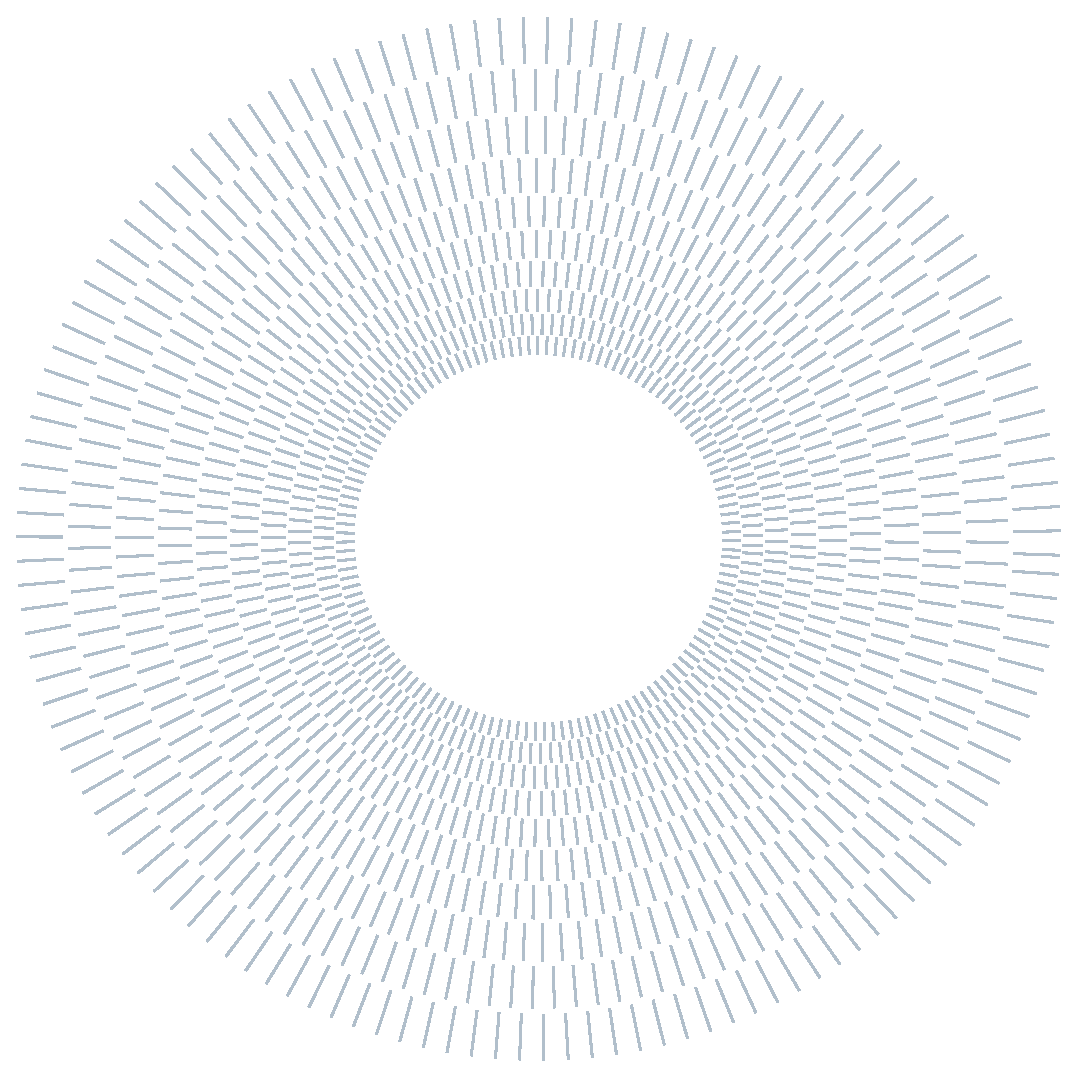
\includegraphics[width=0.7\paperwidth]{raggiera_polimi.eps}%
			\vfill
}}}

% Set indentation
\setlength\parindent{0pt}

% Custom title commands
\titleformat{\section}
{\color{bluePoli}\normalfont\Large\bfseries}
{\color{bluePoli}\thesection.}{1em}{}
\titlespacing*{\section}
{0pt}{2ex}{1ex}

\titleformat{\subsection}
{\color{bluePoli}\normalfont\large\bfseries}
{\color{bluePoli}\thesubsection.}{1em}{}
\titlespacing*{\subsection}
{0pt}{2ex}{1ex}

% Custom headers and footers
\pagestyle{fancy}
\fancyhf{}
      
\fancyfoot{}
\fancyfoot[C]{\thepage} % page
\renewcommand{\headrulewidth}{0mm} % headrule width
\renewcommand{\footrulewidth}{0mm} % footrule width

\makeatletter
\patchcmd{\headrule}{\hrule}{\color{black}\hrule}{}{} % headrule
\patchcmd{\footrule}{\hrule}{\color{black}\hrule}{}{} % footrule
\makeatother

% -> Create the header
\chead[C]{
\centering
\begin{tcolorbox}[arc=0pt, boxrule=0pt, colback=bluePoli!60, width=\textwidth, colupper=white]
    \textsc{\textbf{Executive summary}} \hfill \textsc{\textbf{\author}} 
\end{tcolorbox}
}


% === Start of document ===

\begin{document}
\fancypagestyle{plain}{
\fancyhf{} % Clear all header and footer fields
\fancyhead[R]{\thepage} %RO=right odd, RE=right even
\renewcommand{\headrulewidth}{0pt}
\renewcommand{\footrulewidth}{0pt}}


% === Title page ===
\pagestyle{empty} % No page numbers
\frontmatter % Use roman page numbering style (i, ii, iii, iv...) for the preamble pages

\puttitle{
	title=Ray Distribution Aware Heuristics for Bounding Volume Hierarchies Construction,
	name=Lapo Falcone,
	course=Computer Science and Engineering,
	ID  = 996089,
	advisor= Prof. Marco Gribaudo,
	academicyear={2023-24}
}


% === Preamble ===
\startpreamble
\triangleLogo
\setcounter{page}{1} % Set page counter to 1

% Abstract
\makeatletter
\let\savedchap\@makechapterhead
\def\@makechapterhead{\vspace*{-2cm}\savedchap}
\polimichapter{Abstract}
\let\@makechapterhead\savedchap
\makeatletter

\begin{tikzpicture}[remember picture,overlay,shift={(current page.north west)}]
	\node[anchor=north west]{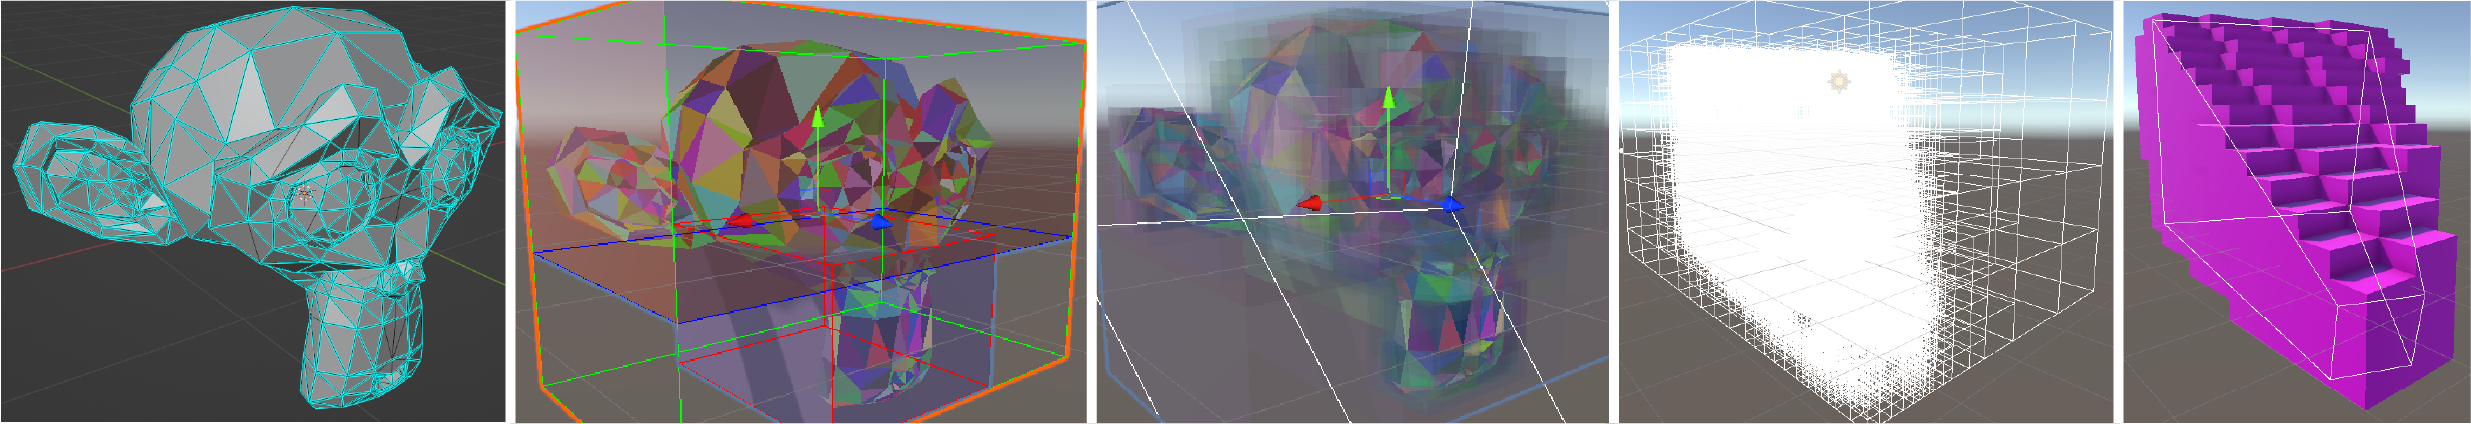
\includegraphics[width=20.7cm]{banner.png}};
\end{tikzpicture}
\begin{tikzpicture}[remember picture,overlay,shift={(current page.south west)}]
	\node[anchor=south west, xshift=2.85cm, yshift=1.8cm]{\textbf{Keywords:} Ray tracing, bounding volume hierarchy, BVH};
\end{tikzpicture}
\vspace{-0.5cm}
\small
\\
In the last few years, real-time computer graphics have been transitioning from a pipeline based on rasterization to one using ray tracing.
Ray tracing makes it possible to accurately simulate the behavior of light rays, enabling developers of graphics content to reproduce high-fidelity scenes without using a plethora of techniques to mimic light transport.

While ray tracing is widely used for off-line rendering, such as for CGI effects in films or animated movies, the same cannot be stated for on-line applications, such as videogames. The main problem with ray tracing is that simulating light transport is computationally expensive, reason why in recent videogames ray tracing is only used on small portions of the scene, or to simulate some effects (such as reflections, shadows, or ambient occlusion).

In order to increase the spread of ray tracing in on-line rendering applications too, research is moving in two macro directions.

The first one is to build GPUs with an architecture more suited for ray tracing, such as the RT cores from Ampere Nvidia GPUs.

The second, but not least important one, is to design software optimizations to make ray tracing cheaper.

One of the problems that is ubiquitous in the ray tracing environment is to detect collisions between a ray and the geometry of the scene to render. Given the huge amount of primitives present in modern graphic applications, it is necessary to use a data structure to accelerate the ray collision retrieval process. The state-of-the-art structure is the Bounding Volume Hierarchy (BVH), which hierarchically organizes primitives, making it possible to skip entire sections of the scene that are spatially far away from the ray that is being traced during BVH traversal.

In this thesis we propose two novel heuristics that work in pair to build higher-quality BVHs, a data structure to make it possible to use them, and a comparative analysis of their performance in different scenarios.

The first heuristic, called \textbf{Projected Area Heuristic} (PAH), aims at better estimating the amount of rays that hit each node of the BVH by exploiting some artifacts in the ray distribution in the scene, caused by another optimization used in a previous step of the ray tracing pipeline (namely Monte-Carlo importance sampling).

The second one, \textbf{Splitting Plane Facing Heuristic} (SPFH) aims at reducing the overlap among nodes of the BVH, consequently reducing the number of intersection tests needed during the BVH traversal phase.

\normalsize

% Abstract in Italian
\makeatletter
\let\savedchap\@makechapterhead
\def\@makechapterhead{\vspace*{-3cm}\savedchap}
\polimichapter{Abstract in Lingua Italiana}
\let\@makechapterhead\savedchap
\makeatletter
\small
Abstract Italiano
\\
\\
\textbf{Parole chiave:} Ray tracing, bounding volume hierarchy, BVH
\normalsize


% === Table of contents ===
\thispagestyle{empty}
\tableofcontents % Table of contents 
\thispagestyle{empty}
\cleardoublepage

\addtocontents{toc}{\vspace{2em}} % Add a gap in the Contents, for aesthetics
\mainmatter % Begin numeric (1,2,3...) page numbering

% Add logo to page numbers
\AddToShipoutPicture{%
	\put(\textwidth+58,\textheight+88){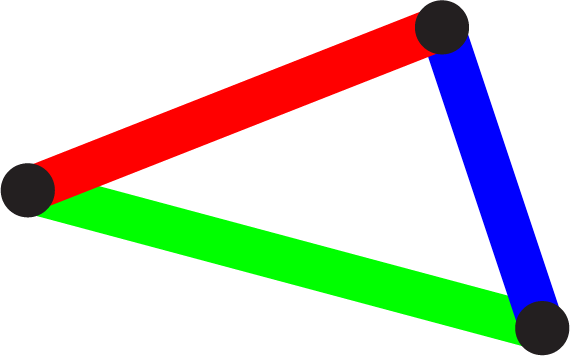
\includegraphics[scale=0.06]{Images/triangle_logo.png}}
}

% === Intro ===
\chapter*{Introduction}
\section*{What Is Ray Tracing}
In the field of computer graphics, we refer to ray tracing as a family of rendering algorithms that simulate light transport, in order to transition from a mathematical representation of a scene to an image on the screen. 

The core algorithm of ray tracing is conceptually simple. First, we cast some rays from each light source in the scene. The rays will collide and bounce away from the objects present in the scene, losing part of their energy. At some point a ray will either lose all of its energy and disappear, or hit the eye of an observer at a specific position. The eye of the observer can be though as a camera, and the position on the camera as the pixel. This means that we can assign a color to the hit pixel, based on the remaining energy of the ray. If more than one ray hits the pixel, the contributions are summed together, if none hits it, the pixel remains black.

\begin{figure}[H]
    \centering
    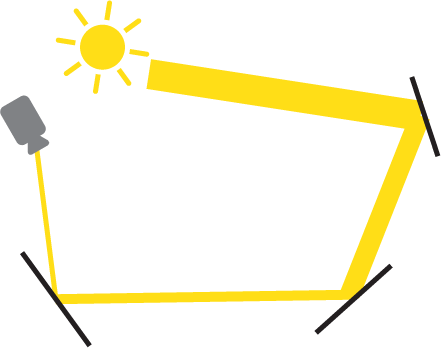
\includegraphics[width=\textwidth*\real{0.4}]{Images/ray_tracing_simple.png}
    \caption{Visualization of the process we described above.}
    \label{fig:ray_tracing_intro}
\end{figure}

The process described above is a simplification of the behavior of the light in real world, and the way in which our brain can see. A lot of different specializations of the ray tracing algorithm exist. Some of them are designed to simulate light very precisely, such as bidirectional path tracing techniques \cite{bidirectional_path_tracing}. Others are designed to be fast.

What all the techniques have in common is the fact that simulating light is an expensive task. The main reason lies in the number of rays that must be cast in order to obtain an accurate rendering of the scene. In the real-world a $100W$ lightbulb is estimated to produce $10^{20}$ photons each second \cite{monte_carlo_integration}. Of course, even in a non real-time scenario, it is computationally impossible to ray trace an image with such an high amount of rays per light. Therefore, one of the most studied research directions in ray tracing is how to reduce the number of photons, while still obtaining an high quality image.

\section*{Monte-Carlo and Kajiya Rendering Equation}
The tool used to achieve this result is Monte-Carlo integration \cite{TODO}. With Monte-Carlo methods it is possible to integrate an arbitrary function with a given amount of random samples. In our case, the function to integrate is inside the Kajiya's rendering equation \cite{rendering_equation}.

The Kajiya's rendering equation is, in summary, a recursive integral equation which calculates the amount of light a point in a scene gets from the surrounding environment. Once we know how much light a point receives, we can compute how much of this energy is reflected toward a given direction, by using the BRDF \cite{brdf}.

One common misconception is that a light ray, after hitting a surface, always bounces towards the perfect reflection direction. This is true only for mirror-like surfaces. Instead, in case the ray hits, for example, concrete, then there is the possibility that the ray bounces in any direction. Each possible bouncing direction has a probability of being chosen by the ray, which is described by the BRDF. In the real-world this happens because, at a microscopic level, a surface is made up of many small facets. This model is described by the micro-facet BRDFs \cite{microfacet_brdf}.

Going back to the Kajiya's rendering equation, as we said, it needs in input the light from the surrounding environment. In order to obtain it, we can cast some probe rays in all directions, which will hit other objects. At this point we can, again, cast some probe rays, and so on, recursively, until a probe ray hits a light source. Now we can reverse the process, by following the probe rays backward, and compute the light hitting a certain point in the scene. The problem lies in the fact that we would need to cast a large amount of probe rays in order to obtain a good approximations of the light incoming to a given point. In other words, we are integrating the light function over the hemisphere oriented toward the surface normal. 

\begin{figure}[H]
    \centering
    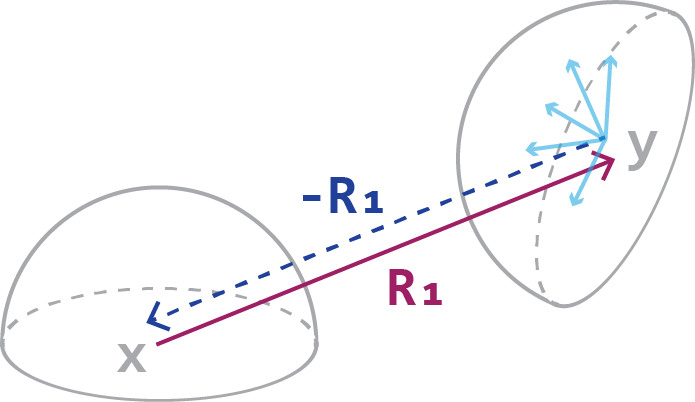
\includegraphics[width=\textwidth*\real{0.4}]{Images/kajiya_recursive.png}
    \caption{Recursiveness of Kajiya's rendering equation.}
    \label{fig:rendering_equation_recursive_intro}
\end{figure}

What we described in the previous paragraph is a simplification of the Monte-Carlo method. With Monte-Carlo we have the mathematical proof that we can obtain a good estimate of the light incoming to a point by following this process, which involves the random sampling of the directions where to cast the probe rays.

Monte-Carlo variance reduction techniques, such as importance sampling \cite{importance_sampling}\cite{multi_light_sampling}, help us to achieve a precise approximation of the light incoming to a point with a low amount of probe rays, which is the goal we set.

However, importance sampling, creates artifacts in the distribution of the probe rays in the scene. If, with plain Monte-Carlo, the rays are distributed uniformly in the scene, by using importance sampling their distribution changes, and more rays tend to go toward light sources. This effect is the main hypothesis of the the novel heuristics we propose in this work.

\section*{Bounding Volume Hierarchies}
Another fundamental task that any ray tracing algorithm must perform, is to find the intersection between a ray and the geometry of the scene. Usually the objects in the scene are described as surfaces made up of a big number of small triangles. Therefore, finding the intersection of a ray with a scene, reduces to finding the intersection between a ray and a large amount of triangles.

One way to do so is by using the brute-force approach: for each ray, we perform the ray-triangle intersection test with each triangle. If we have $n$ rays and $m$ triangles, $m*n$ intersection tests must be carried out.

Considering that we need a lot\footnote{at least one per pixel, at least $1080 \cdot 1920 = 2073600$ on HD displays.} of rays to achieve realistic images, and that we need a lot of triangles design accurate objects, the brute-force method is too slow.

A better way to perform ray-scene intersection is to organize the triangles in a hierarchical fashion. We can first divide the scene into two sections, and delimit each one with a parallelepiped (an Axis-Aligned Bounding Box, or AABB): if the ray doesn't hit one of the two, we can exclude all the triangles present in that part of the scene. Bounding Volume Hierarchies (BVHs) extend this simple idea recursively. First the scene is divided into two parts; then each one of the two parts, is further divided into two sub-parts, and so on. The structure originating from this process is a binary tree. This means that, in order to perform ray-scene intersection, on average only $log_2 n \cdot m$ intersection tests are needed.

\begin{figure}[]
    \centering
    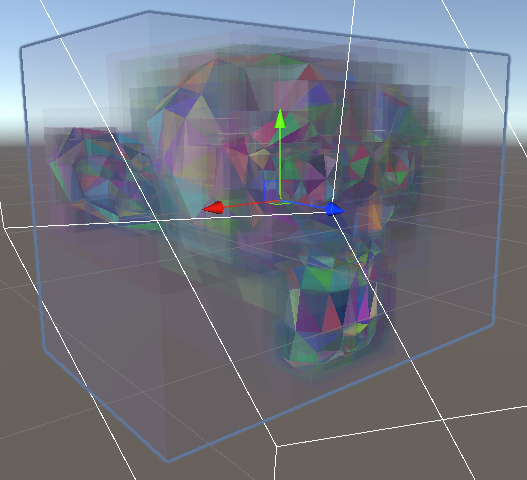
\includegraphics[width=\textwidth*\real{0.55}]{Images/suzanne_visualizer.png}
    \caption{A BVH built with our heuristics over a radial ray distribution, as displayed by our Unity visualizer.}
    \label{fig:suzanne_intro}
\end{figure}

One of the main concerns while building a BVH is how to split a BVH node into two parts so that the final binary tree actually allows to achieve the logarithmic complexity we described, during traversal. The idea is to group triangles that are close together, while minimizing the surface area of the two resulting AABBs. This heuristic is called Surface Area Heuristic (SAH), and is applied at each level of the BVH while it is built. SAH tries to estimate the probability an AABB is hit, and reduce it to the minimum, even though by using a greedy algorithm, due to time constraints.

SAH works under the hypothesis that the ray distribution in the scene is uniform. However, as we described in the previous section, we know that, due to Monte-Carlo importance sampling this is not the case.

By leveraging this finding, we propose two novel heuristics that are aware of some ray distributions in the scene, and use this knowledge to take better decisions while building the BVH.

The ray distributions our heuristics take into consideration are two: parallel ray distribution, and radial ray distribution.

Parallel ray distributions are usually found in proximity of planar area light sources, where, as the name suggests, rays tend to be parallel among them, and perpendicular to the light source. By knowing the presence of this distribution, we can try to estimate better the probability a ray hits an AABB present in that region. Indeed, if all rays are parallel, we know that only some faces of the AABB can be hit, while faces facing away from the camera can never be hit. Knowing this, we state that the probability of an AABB to be hit by a ray is proportional to the area of the polygon obtained by projecting it to a plane perpendicular to the rays. In other words, we use an orthographic projection to project the AABB to the planar area light, and compute the area of the projection.

For what concerns radial ray distributions, they tend to be present near point light sources, such as spotlights. In this case all the rays pass through the point light, forming a radial distribution over a certain solid angle. In this case, we estimate the hit probability by using a perspective projection, with focal point the position of the light source.

We call this heuristic to approximate the probability an AABB is hit Projected Area Heuristic (PAH).

The second novel heuristic we propose, takes into account the same distributions as PAH, but, instead of estimating the hit probability, it tries to minimize the overlapping between sibling nodes.

Let's think about parallel ray distribution. If we try to divide a node in this region into two children with a plane perpendicular to the rays, it is almost certain that the ray will hit both the children. This happens because the two children have a large overlapping area, when projected. If, instead, we cut the node with a plane parallel to the rays, the overlapping will be much smaller in many cases.

We call this method Splitting Plane Facing Heuristic (SPFH), as opposed to the state-of-the-art Longest Splitting Plane Heuristic (LSPH), where a node is always cut perpendicular to its longest side.

\begin{figure}[H]
    \centering
    \subfloat[Perpendicular plane]{
        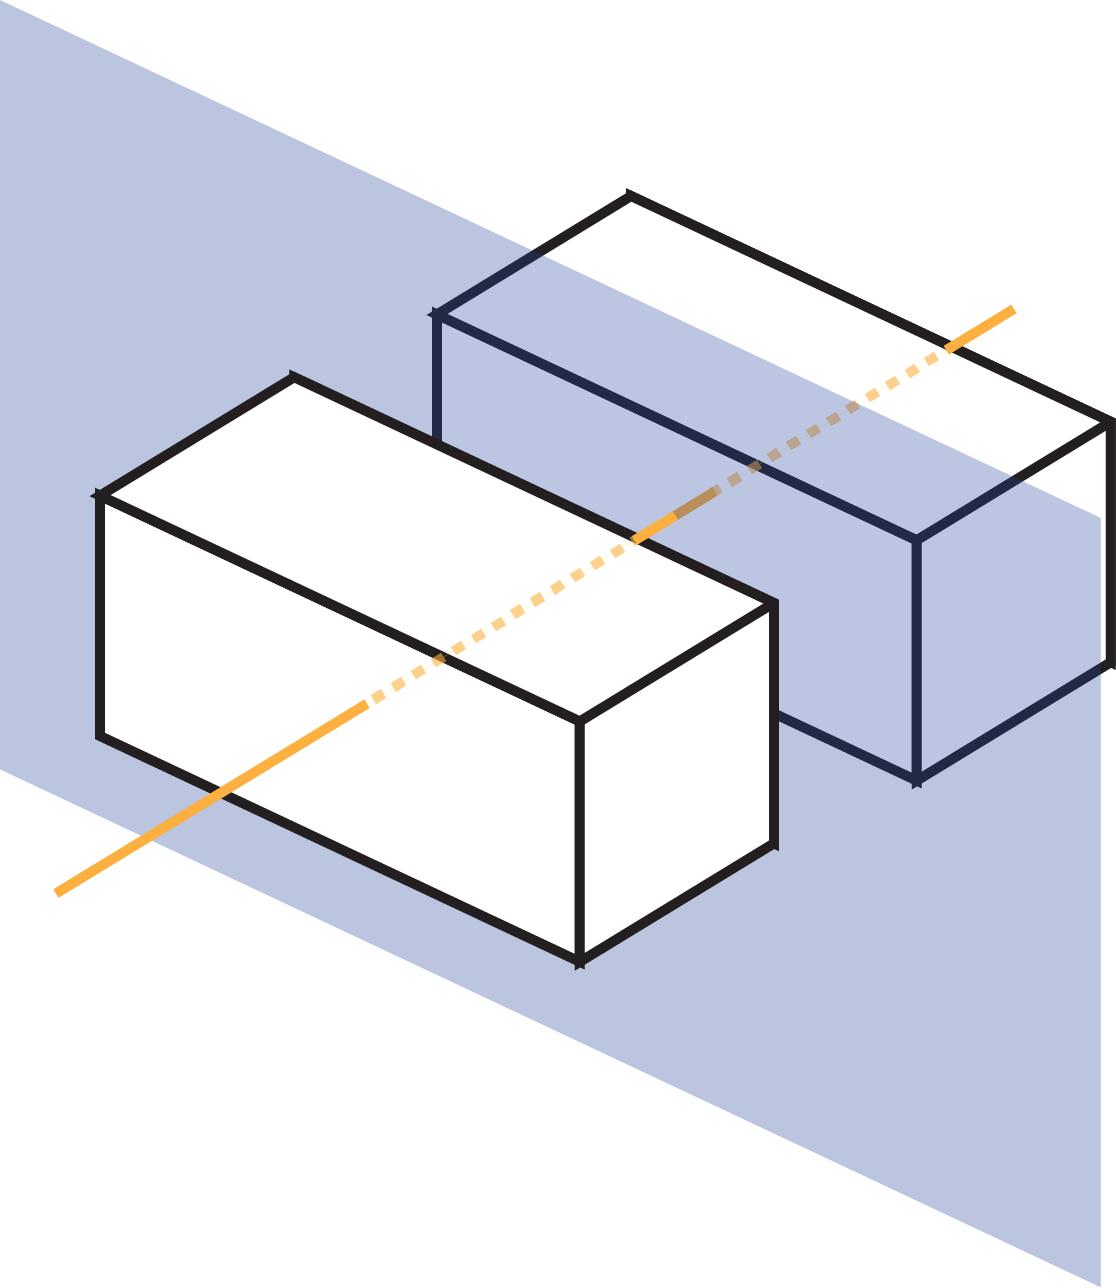
\includegraphics[width=\textwidth*\real{0.35}]{Images/z_axis_plane.png}
	}
	\qquad
	\subfloat[Parallel plane]{
        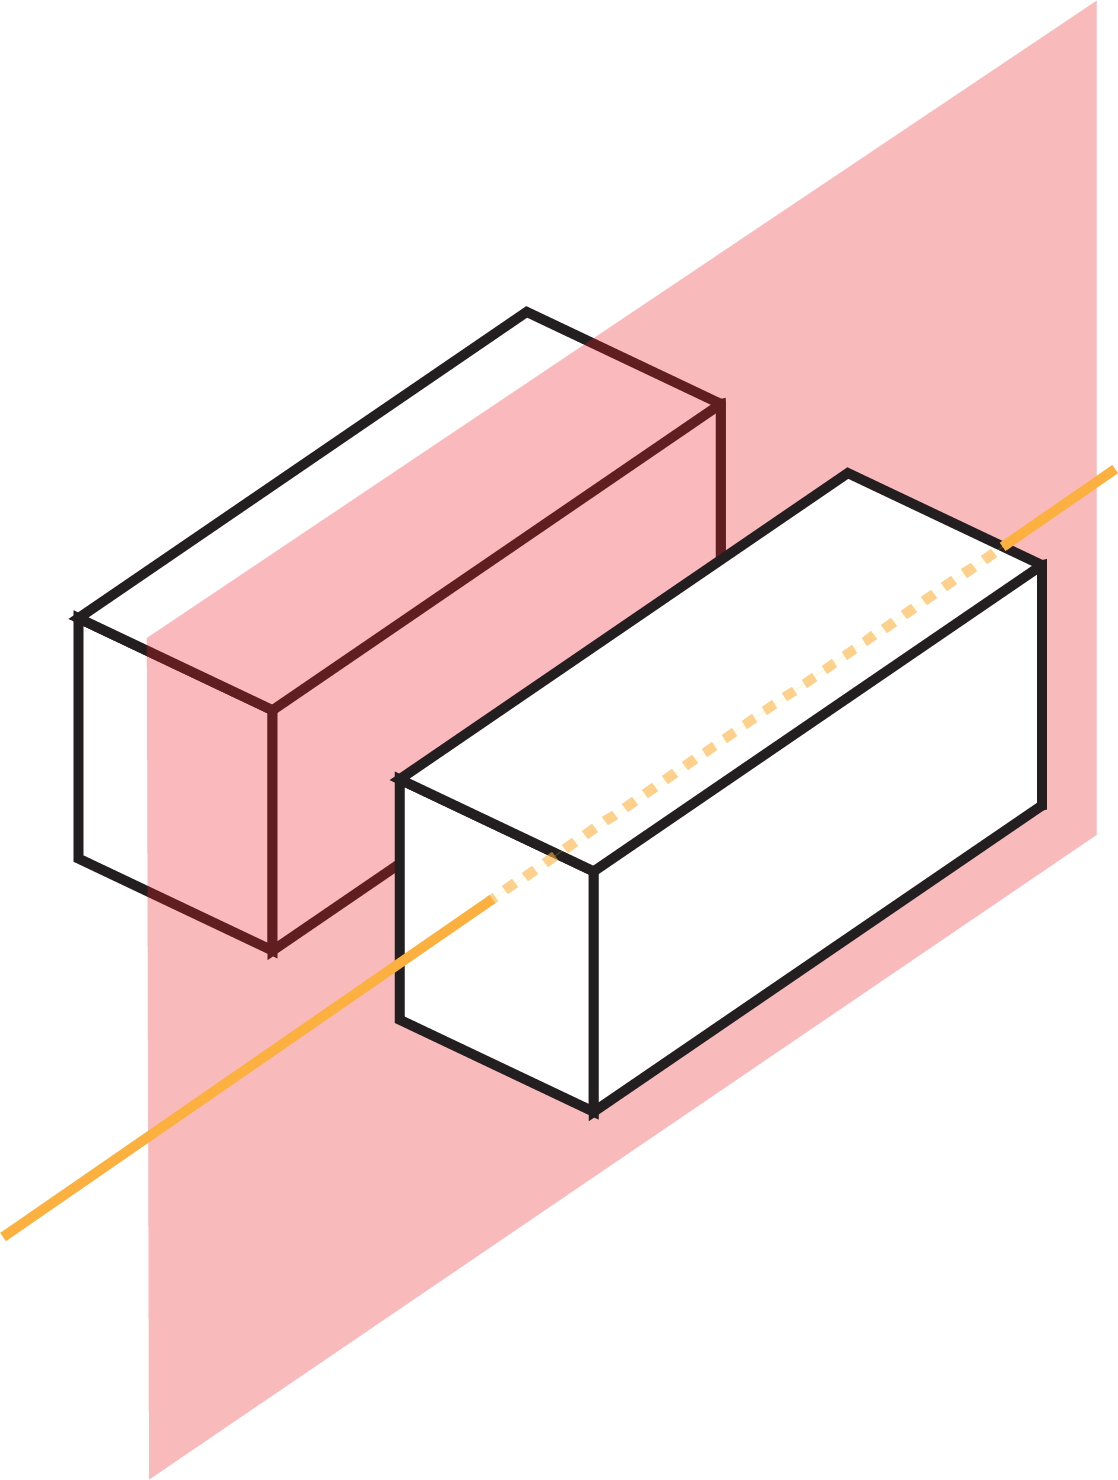
\includegraphics[width=\textwidth*\real{0.35}]{Images/x_axis_plane.png} 
    }
	\caption{How a node can be split. SPFH would choose the parallel plane}
    \label{fig:nodes_splitting_intro}
\end{figure}

\section*{Top Level Structure}
If we build a BVH using SAH and LSPH, the information required by the heuristics are uniform in all of the scene, therefore just one BVH can be built. However, PAH and SPFH inherently divide the scene in local regions, where the relevant ray distributions are present. For this reason, we need a top level structure in order to find out whether, given a ray, it is \textit{affine} with a certain ray distribution present in the scene, and can therefore be traced against the associated BVH.

With the term \textit{affine} we refer to the fact that, not only the ray origin must be inside the region where a certain distribution is present, but also its direction must be \textit{similar} to the directions of the rays present in the distribution.

The easier way to find out if a ray origin is in a certain region, is testing if the point is inside each distribution region present in the scene. However, this doesn't scale, therefore we decided to implement an octree structure.

Once we know that a ray origin is inside a certain ray distribution region, it is fast to check whether its direction is similar to the one of the distribution.

\begin{figure}[]
    \centering
    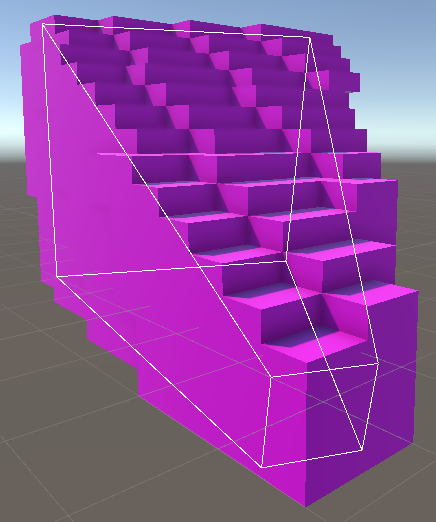
\includegraphics[width=\textwidth*\real{0.45}]{Images/octree_visualizer.png}
    \caption{An octree as displayed by our Unity visualizer.}
    \label{fig:octree_intro}
\end{figure}

\section*{Thesis Outline}
\begin{itemize}
	\item In chapter \ref{ch:background_theory} we will introduce the research context our thesis is part of, and we will explain the theory that is needed to fully understand our work. The focus will be on the parts that are operationally relevant, and we will try to highlight them with concrete examples, along with more rigorous mathematical proofs where needed. In particular we talk about the foundations of ray tracing, the Monte Carlo integration method and a variance reduction technique called importance sampling. Eventually we will explain what a ray tracing acceleration structure is, and why BVHs are the most popular ones.
	\item In chapters \ref{ch:projected_area_heuristic}, \ref{ch:multi_influence_areas} and \ref{ch:splitting_plane_facing_heuristic} we will expose our novel heuristics to improve the building of BVHs in some specific scenarios. In these chapters we will mainly explain the theory, and we will only briefly talk about our implementation. The implementation will be diffusely discussed in chapter \ref{ch:implementation}.
	\begin{itemize}
		\item In chapter \ref{ch:projected_area_heuristic} we will detail the first novel heuristic we propose: the surface area heuristic (SAH). SAH aims at better estimating the quality of a BVH, in order to be able to make better decisions during the building phase.
		\item In chapter \ref{ch:multi_influence_areas} we will describe the data structures needed to enable the use of SAH, from a theoretical point of view.
		\item In chapter \ref{ch:splitting_plane_facing_heuristic} we will explain the second novel heuristic, called splitting plane facing heuristic (SPFH). SPFH is focused on the selection of the best plane to split the triangles during BVH construction.
	\end{itemize}
	\item In chapter \ref{ch:implementation} we will extensively explain the implementation details we omitted from the previous three chapters. We decided to subdivide the thesis like this for two main reasons: do not overload the theory chapters, in order to be able to concisely get to the core concepts; and leave the reader with a section where all the implementation details are concentrated, so that, in case he or she wants to try our framework, this section can be used as a reference.
	\item In chapter \ref{ch:experimental_results} we will show the experimental results related to our heuristics, which we omitted or only briefly mentioned in the previous chapters. We will test our theory with the framework described in the previous chapter, and compare the results with those obtained by using different parameters or scenes, and also with the results obtained by using the state-of-the-art heuristics, namely the Surface Area Heuristic (SAH) and the Longest Splitting Plane Heuristic (LSPH).
	\item In chapter \ref{ch:conclusion} we will list some possible scenarios where our techniques can be effectively used, based on the results obtained in the previous section. Moreover, we will produce a list of possible future development directions for the novel topics discussed in our thesis. Eventually, we will draw the main take-away points of our work.
\end{itemize}


\chapter{Background Theory}
\label{ch:background_theory}
In this chapter we will summarize the background knowledge needed to fully comprehend this work.

In section \ref{sec:ray_tracing_principles} we will introduce ray tracing in simple terms, and list some of its advantages, disadvantages and its today's applications.

In section \ref{sec:monte_carlo_and_variance_reduction_techniques} we will analyze from a mathematical standpoint how the most used ray tracing algorithms work.

Last, in section \ref{sec:ray_tracing_acceleration_structures}, we will describe the state-of-the-art acceleration structure to make a fundamental ray tracing procedure (ray-scene intersection) faster.

\section{Ray Tracing Principles} \label{sec:ray_tracing_principles}
Ray tracing is a family of rendering algorithms that is used in computer graphics to transition from a mathematical representation of a scene, to an image on the screen.

Conceptually ray tracing is an extremely straightforward technique, that can be summarized in a few steps:
\begin{enumerate}
\item Generate a ray of light from a light source;
\item Find out the first object the ray intersects;
\item Compute how much energy is absorbed by the material of the object;
\item Modify the direction of the ray based on the material of the object (for example it may be reflected or refracted);
\item Repeat from 2. until the ray hits the camera or loses all its energy;
\item Color the pixel of the camera hit by the ray based on the energy of the ray.
\end{enumerate}

Ray tracing aims to mimic the real-world behavior of light, and for this reason it can be directly employed to simulate any light effect, starting from the simplest ones, such as perfect reflections and shadows, going towards the most complex ones, such as global illumination and caustics. Some of the most accurate ray tracing algorithms can even simulate quantum effects of light \cite{quantum_ray_tracing}.

Since ray tracing natively simulates light, it can produce extremely realistic images, without resorting to ad-hoc techniques used to approximate light phenomena in other rendering algorithms, such as the widely spread rasterization pipeline.

To give an intuition of how the ad-hoc methods can be convoluted and produce worse results, we summarize one of the simplest ones used to generate shadows, called shadow mapping \cite{shadow_maps}. A shadow map is the projection of the scene from the point of view of a point light source, saved in a texture where each pixel stores the distance from the light source to the projected point. When the scene is projected by the main camera, each visible point is transformed into the coordinate system of the shadow map via matrix multiplication (figure \ref{fig:shadow_map}). The point in the new coordinate system is then compared to the point stored in the corresponding pixel of the shadow map. If the point of the shadow map is closer to the light source than the corresponding point projected by the main camera, we deduce that such a point is not visible from the point of view of the light source and, therefore, is in shadow. This specific technique is correct only with point lights, and must be adjusted in case translucent objects are present in the scene.

With ray tracing shadows are natively generated since, if a point is in shadow, no light ray starting from it will hit the camera pixels. Moreover, in principle, it works with any kind of light, not only point lights, and thus produces higher-quality shadows, since no approximations must be made.

\begin{figure}[]
    \centering
    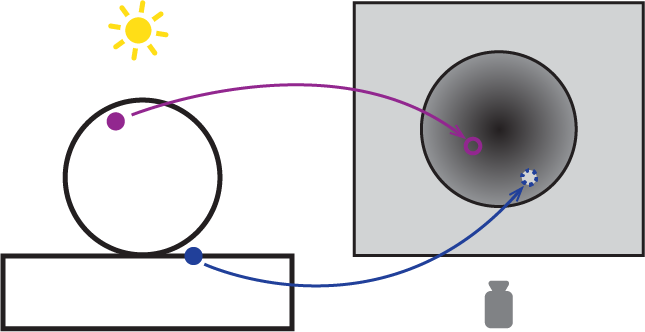
\includegraphics[width=\textwidth*\real{0.65}]{Images/shadow_map.png}
    \caption{The first figure is from the main camera PoV, the second one from the light source PoV. The second figure represents depth: the closer a point is to the light source, the darker. The blue point is in shadow, because the corresponding point in the shadow map is further away than the stored depth.}
    \label{fig:shadow_map}
\end{figure}

\subsection{Use Cases}
Due to the highly realistic images ray tracing algorithms can produce, the technique has found a lot of success in many applications. We can subdivide the use cases into two macro-categories: real-time ray tracing and production ray tracing.

The most prominent use of the second category is in movies. CGI effects and animated films are almost always produced by using ray tracing \cite{path_tracing_movies}, in particular a very accurate algorithm called bi-directional path tracing \cite{bidirectional_path_tracing}. In the first category we can find videogames.

The main difference between real-time and production ray tracing lies in the time constraints for producing a frame. In production ray tracing producing a frame can take a long time, even in the order of magnitude of days. Whereas, in real-time ray tracing, a frame must be produced every $33$ms to achieve $30$ frames per second (fps), and every $16.5$ms to achieve $60$ fps, which can be considered today's standard by many PC videogames.

This striking difference makes it so that different techniques must be used depending on the scenario. In real-time ray tracing many approximations must be introduced in order to stay within the frame time budget, whereas in production ray tracing more accurate algorithms can be used, since time constraints are loose. Our work can benefit both categories, since the methods we will introduce can make ray tracing faster, in some situations, without introducing approximations.

\subsection{Optimizations Overview} \label{ssec:optimizations_overview}
Until now we briefly highlighted the strong points of ray tracing, and greatly simplified it. The main issue with ray tracing is that it is computationally expensive to simulate light transport in a convincing way. The reason lies in the rendering equation, and will be explained in section \ref{sec:monte_carlo_and_variance_reduction_techniques}.

In order to make ray tracing usable in the real world, the industry moved in two directions:
\begin{description}
	\item [Hardware accelerators] GPU vendors, in particular Nvidia, started creating GPUs with specialized cores for ray tracing. These cores have a memory layout that makes it faster to find a ray-triangle intersection. An example of this can be the RT cores from Turing Nvidia GPUs \cite{rt_cores}.
	\item [Software optimizations] Software developers introduced new algorithms to improve the performance of a specific part of the ray tracing pipeline. These algorithms can vary a lot in complexity and results. One of the most common optimizations for real-time ray tracing is to use ray tracing only for some light effects (such as shadows or reflections), while using rasterization for most of the scene.
\end{description}

Software optimizations can, in turn, be subdivided into two big families.

Some optimizations aim at improving the time needed to detect the first intersection of a ray with the scene, without altering the quality of the rendered scene. We will diffusely talk about these optimizations in section \ref{sec:ray_tracing_acceleration_structures}, and this work can be placed into this family.

The other family comprehends optimizations aimed at reducing the number of rays needed to produce a visually acceptable image. This work, while being part of the first family of optimizations, has its foundations in an artifact in the ray distribution in the scene caused by an optimization of this second family. This technique is called importance sampling, and will be discussed in section \ref{sec:monte_carlo_and_variance_reduction_techniques}.

\subsection{Backward Ray Tracing}
Before going to the next section, it is important to introduce the concept of backward ray tracing\footnote{In some literature the term \textit{backward ray tracing} can also refer to the opposite family of algorithms, since the first ray tracing methods were indeed backward.}. 

In backward ray tracing light rays don't start from light sources, but from the eye position. Starting from the eye, each ray will then hit a fictitious plane placed in front of the eye (the near plane), similar to what happens in a pinhole camera \cite{pinhole_camera}. The near plane can be subdivided into discrete units displaced in a regular grid, which we will consider the pixels of the final image. Each ray is therefore associated with the pixel it hits, and will contribute to its final color.

\begin{figure}[H]
    \centering
    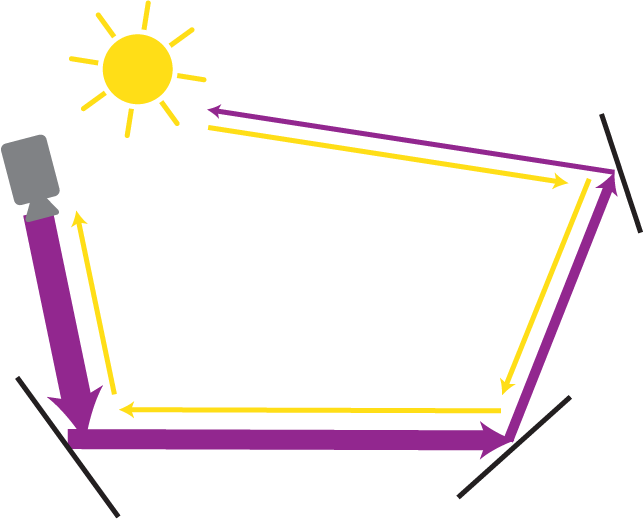
\includegraphics[width=\textwidth*\real{0.4}]{Images/backward_ray_tracing.png}
    \caption{How rays are cast in backward ray tracing.}
    \label{fig:pinhole_camera}
\end{figure}

The rays starting from the camera will hit the scene and bounce around. At each bounce a ray loses a fraction of its energy (unless the surface is perfectly reflective), until either it gets completely absorbed, or it hits a light source. In the case a ray hits a light source, we already know how much of its energy will be lost due to intersections with objects, therefore we can immediately compute the color of the pixel associated with the ray, as if we followed that same ray's path backward. If a ray never hits a light source, it will not contribute to the color of its associated pixel, because it never gain energy.

A way of looking at this algorithm is to think we are tracing \textit{importons}, which can be considered the dual concept of \textit{photons} \cite{importons}. Thanks to the light reciprocity principle \cite{light_reciprocity}, which states that light transmits in the same way in both directions, tracing photons or importons is equivalent.

The advantage of backward ray tracing is that, with a limited budget of rays we can cast, it is more efficient than forward ray tracing. Indeed, in forward ray tracing it is possible a ray never hits the camera, in which case it would be wasted. In backward ray tracing all the rays hit the camera by definition, thus none is wasted.

Of course, if a ray starting from the camera never hits a light source, it could be considered wasted, but some techniques that will be described in section \ref{sec:monte_carlo_and_variance_reduction_techniques} make it more likely for a ray to hit a light source in its path.

From this point on, we will consider the scenario where rays are traced backwards.

\section{Monte-Carlo and Variance Reduction Techniques} \label{sec:monte_carlo_and_variance_reduction_techniques}
In this section we will analyze the mathematical foundations of ray tracing, namely Kajiya's rendering equation. Then we will present a statistical method to resolve the integrals appearing in the rendering equation, called Monte-Carlo. Finally, we will discuss a variance reduction technique, importance sampling, that can be used to obtain better approximations from the Monte-Carlo method, without making it more expensive. We will see how this technique generates artifacts in the ray distribution in the scene, which is one of the hypotheses of our thesis.

\subsection{Kajiya's Rendering Equation}
$$
L_o(\bar{x},\bar{\omega}_o) = L_e(\bar{x}, \bar{\omega}_o) + \int_\Omega BRDF(\bar{x}, \bar{\omega}_i, \bar{\omega}_o) \cdot \cos(\bar{n}, \bar{\omega}_i) \cdot L_i(\bar{x}, \bar{\omega}_i) d\bar{\omega}_i
$$

This equation, developed by James T. Kajiya in 1986 \cite{rendering_equation}, can be used to calculate the amount of light \textit{generated} by a point $\bar{x}$ towards a direction $\bar{\omega}_o$. As we will see in the next paragraphs, with the term \textit{generated} we refer to the sum of the light emitted by the point, and the light reflected by it. In order to compute the \textit{generated} light we need to know these variables:
\begin{itemize}
	\item $L_e(\bar{x}, \bar{\omega}_o)$ The light emitted by the point $\bar{x}$ towards a direction $\bar{\omega}_o$.
	\item $BRDF$ The bidirectional reflectance distribution function of the material at point $\bar{x}$.
	\item $\bar{n}$ The normal to the surface at point $\bar{x}$.
	\item $L_i(\bar{x}, \bar{\omega}_i)$ The light incoming to $\bar{x}$ from a generic direction $\bar{\omega}_i$ on the hemisphere $\Omega$ orientated toward $\bar{n}$.
\end{itemize}

The equation can be divided into two parts:

The first part describes the light emitted $L_e(\bar{x}, \bar{\omega}_o)$, and it is 0 unless the point is a light source. Depending on the light source type, it can assume a uniform value in each direction (point light), a value only in one hemisphere (a plane area light), or a specific value based on the direction, usually controlled by a function (such as in spotlight). In any case the emitted light value is known by the definition of the light source in the scene, therefore can be easily plugged into the equation.

\begin{figure}[H]
    \centering
    \subfloat[Point light]{
        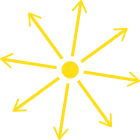
\includegraphics[width=\textwidth*\real{0.15}]{Images/point_light.png}
	}
	\qquad
	\subfloat[Area light]{
        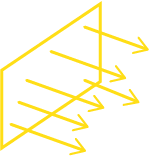
\includegraphics[width=\textwidth*\real{0.15}]{Images/plane_light.png} 
    }
	\qquad
	\subfloat[Spotlight]{
        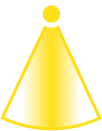
\includegraphics[width=\textwidth*\real{0.13}]{Images/spot_light.png}
    }
	\caption{Three possible types of light sources.}
    \label{fig:light_sources}
\end{figure}

The second part of the equation presents an integral, and represents the light reflected by the material of the point towards the direction $\bar{\omega}_o$. In simple words, this second term tells us that, in order to compute the reflected light, we have to know, first, how much light is incoming to the point from all the directions in the hemisphere $\Omega$. And second, the properties of the material, summarized in the $BRDF$ \cite{brdf}. The $BRDF$ tells us how much of the incoming light is reflected towards the direction $\bar{\omega}_o$. 

\begin{figure}[H]
    \centering
    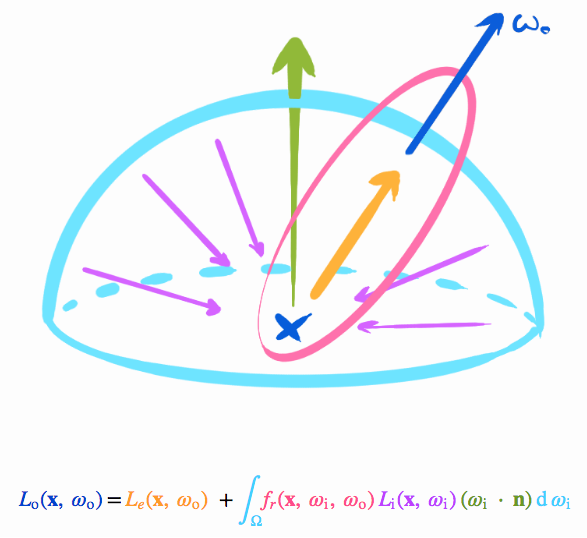
\includegraphics[width=\textwidth*\real{0.5}]{Images/kajiya_visual.png}
    \caption{A visual representation of the Kajiya rendering equation from \cite{kajiya_equation_drawing}.}
    \label{fig:rendering_equation}
\end{figure}

The term $\cos(\bar{n}, \bar{\omega}_i)$ is called geometry term, and reflects a core property of light, independent of the $BRDF$. Indeed, based on the angle a beam of light intersects a surface, the beam of light will enlighten a smaller or bigger area of the surface. The smallest surface is illuminated when the direction of the beam of light and the normal to the surface are parallel. Since the energy carried by the beam of light is constant, we can deduce that, the bigger the enlightened surface, the lower the energy per area unit. In particular, if we let $L$ be the energy of the beam and $\alpha$ the angle between the beam direction and the normal, then the energy received per area unit equals to $L\cdot \cos(\alpha)$. 

\begin{figure}[H]
    \centering
    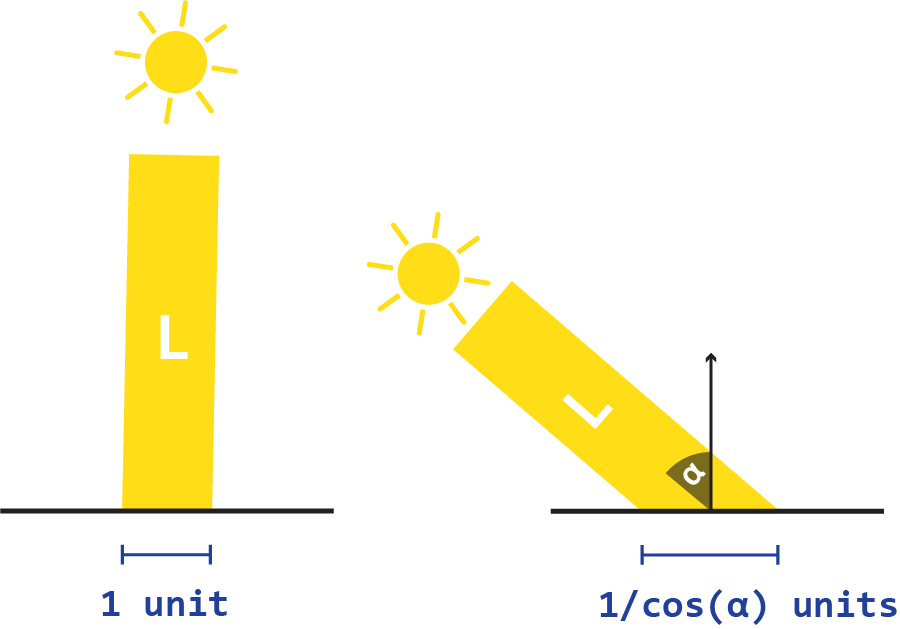
\includegraphics[width=\textwidth*\real{0.45}]{Images/geometry_term.png}
    \caption{The geometry term.}
    \label{fig:geometry_term}
\end{figure}

When we compute the integral term of the rendering equation, the BRDF is known by definition, and the geometry term is a simple cosine. On the other hand, we almost never have an analytical form of the $L_i$ term, and it is indeed this specific part of the equation what really makes ray tracing expensive.

In order to compute the $L_i$ term for one specific direction $\overline{\omega_{\tilde{i}}}$, we can cast a probe ray $R_1$ from point $\overline{x}$ toward $\overline{\omega_{\tilde{i}}}$. The probe ray will hit another point $\overline{y}$. Now, since we want to compute how much light $R_1$ is carrying towards $\overline{x}$, we have to resolve the rendering equation at point $\overline{y}$ and with outgoing direction $-\overline{\omega_{\tilde{i}}}$, namely $L_o(\overline{y}, -\overline{\omega_{\tilde{i}}})$. In other words, the light incoming to one point from one direction, equals the light outgoing from a second point towards the same direction, with inverted sign. This recursive pattern is usually ended after a certain number of bounces (when we can consider that the ray is carrying an infinitesimal amount of energy), or when a probe ray hits a light source (where the generated light is only influenced by the emitted light term of the rendering equation).

\begin{figure}[H]
    \centering
    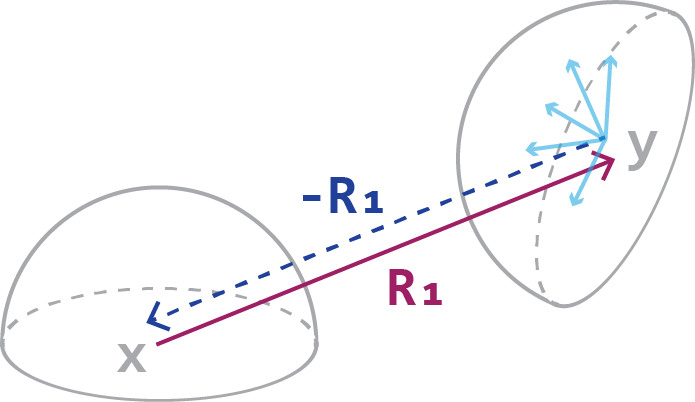
\includegraphics[width=\textwidth*\real{0.45}]{Images/kajiya_recursive.png}
    \caption{Recursiveness of the integral term of the Kajiya rendering equation.}
    \label{fig:kajiya_recursiveness}
\end{figure}

The process we've just described only returns the amount of light incoming to $\overline{x}$ from an arbitrary direction $\overline{\omega_{\tilde{i}}}$. But, as we can see, in the rendering equation an integral over the hemisphere $\Omega$ is present, therefore, in order to have a mathematically correct result, we would need to cast an infinite amount of probe rays. This is not feasible, and leads us to the Monte-Carlo method.

\subsection{Monte-Carlo Integration} 
In this section we will provide an intuition of the Monte-Carlo integration method, and its basic mathematical foundations necessary to fully understand this work.

Monte-Carlo integration \cite{monte_carlo_integration} is a method by which it is possible to compute the numerical integral of a function by using random samples.
Given a one-dimensional positive integrable function $f$, we can interpret its definite integral in the $[a,b]$ interval as the area between the curve and the x-axis.
Now, if we select a random point $k_0$ uniformly in the $[a,b]$ interval, we can compute the area $A_r$ of the rectangle with side $\overline{ab}$ and height $f(k_0)$ as $\overline{ab} \cdot f(k_0)$. We can interpret it as a very rough approximation of the area under the function, which, by definition, is equal to the definite integral value. If we repeat this process $N$ times and compute the average of the various $A_r$s, we'll usually get a better estimate of the area under the function, because sometimes we will underestimate its value, and sometimes we will overestimate it.

\begin{figure}[H]
    \centering
    \subfloat[Area approximation with one sample.]{
        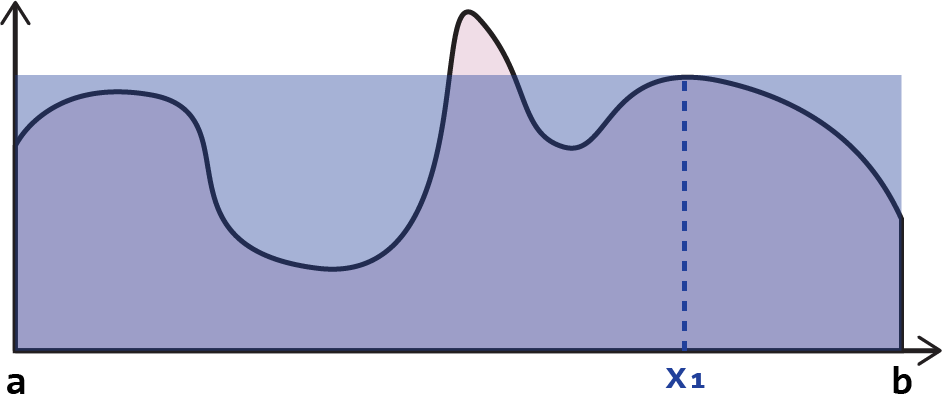
\includegraphics[width=\textwidth*\real{0.65}]{Images/monte_carlo_area_1x.png}
	}
	\qquad
	\subfloat[Area approximation with 4 samples]{
        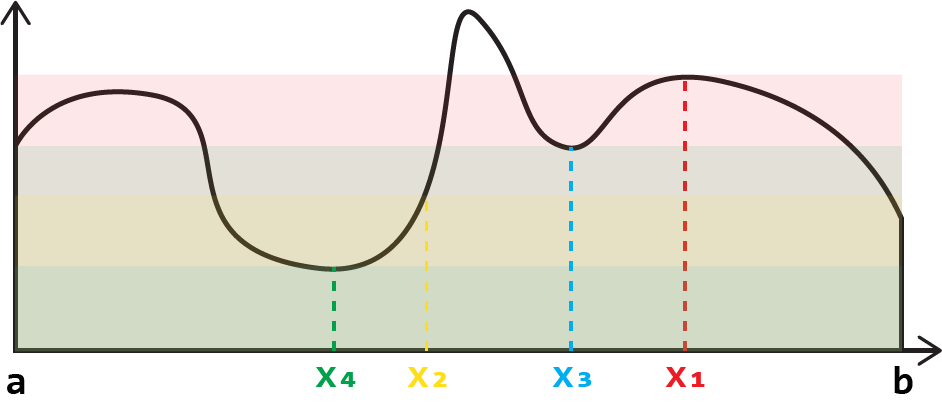
\includegraphics[width=\textwidth*\real{0.65}]{Images/monte_carlo_area_4x.png}
    }
	\caption{Monte-Carlo area approximation. When we hame many samples, sometimes the area will be overestimated, some other times underestimated.}
    \label{fig:monte_carlo_area_approximation}
\end{figure}

We can formalize this process with this formula, where $X_i \sim \frac{1}{b-a}$ is a uniform random variable in the $[a,b]$ interval. 

$$\langle F^N \rangle = \frac{1}{N}\cdot (b-a)\cdot\sum_{i=0}^{N-1}\textit{f}(X_i)$$

$\langle F^N \rangle$ is referred to as the basic Monte-Carlo estimator \cite{monte_carlo_estimators_veach} \cite{monte_carlo_estimators_scratchapixel}. The Monte-Carlo estimator, being a linear combination of random variables, is a random variable itself. Monte-Carlo theory states that the expected value of the Monte-Carlo estimator equals the definite integral of $f$. Below we prove this statement:

\begin{subequations}
	\begin{align*}
		E[\langle F^N \rangle] &= E[(b-a)\cdot \frac{1}{N}\sum_{i=0}^{N-1}\textit{f}(X_i)] \\
		&= (b-a)\cdot \frac{1}{N}\cdot\sum_{i=0}^{N-1} E[\textit{f}(X_i)] \\
		&= (b-a)\cdot \frac{1}{N}\cdot\sum_{i=0}^{N-1}\int_{a}^{b}\textit{f}(x) \cdot \frac{1}{b-a} dx \\
		&= \frac{1}{N}\cdot\sum_{i=0}^{N-1}\int_{a}^{b}\textit{f}(x) dx \\
		&= \int_{a}^{b}\textit{f}(x) dx
	\end{align*}
\end{subequations}

In order to go from line 2 to line 3, it is important to remember the law of the unconscious statistician (LOTUS) \cite{lotus}, where $p$ is the probability density function of the random variable $X$:
$$E[\textit{f}(X)] = \int_{\Omega}\textit{f}(x)\cdot p(x) dx$$ 

The LOTUS is easier to understand in its discrete case, where $E[\textit{f}(x)] = \sum\textit{f}(x)\cdot p(x)$. This can, for example, be visualized to compute the expected value of a fair die throw: each side has $\frac{1}{6}$ chances of appearing, therefore the expected value equals: $\frac{1}{6} \cdot 1 + \frac{1}{6} \cdot 2 + \frac{1}{6} \cdot 3 + \frac{1}{6} \cdot 4 + \frac{1}{6} \cdot 5 + \frac{1}{6} \cdot 6 = 3.5$. If the die was unfair and, for example, $6$ has a probability to appear of $\frac{1}{2}$, and the remaining 5 sides have a probability of $\frac{1}{10}$ then the expected value would be skewed towards high numbers: $\frac{1}{10} \cdot 1 + \frac{1}{10} \cdot 2 + \frac{1}{10} \cdot 3 + \frac{1}{10} \cdot 4 + \frac{1}{10} \cdot 5 + \frac{1}{2} \cdot 6 = 4.5$. 

Monte-Carlo integration can be used even if the random variable $X_i$ follows a non-uniform distribution. Let the Probability Density Function (PDF) of $X_i$ be $p$, then the Monte-Carlo estimator can be written as \cite{monte_carlo_estimators_veach} \cite{monte_carlo_estimators_scratchapixel}:

$$\langle F^N \rangle = \frac{1}{N}\cdot\sum_{i=0}^{N-1}\frac{\textit{f}(X_i)}{p(X_i)}$$

We can prove the formula with an analogous proof to the one above (this time the integration domain is $\Omega$): 

\begin{subequations}
	\begin{align*}
		E[\langle F^N \rangle] &= E[\frac{1}{N}\cdot\sum_{i=0}^{N-1}\frac{\textit{f}(X_i)}{p(X_i)}] \\
		&= \frac{1}{N}\cdot\sum_{i=0}^{N-1}E[\frac{\textit{f}(X_i)}{p(X_i)}] \\
		&= \frac{1}{N}\cdot\sum_{i=0}^{N-1}\int_{\Omega}\frac{\textit{f}(x)}{p(x)} \cdot p(x) dx \\
		&= \frac{1}{N}\cdot\sum_{i=0}^{N-1}\int_{\Omega}\textit{f}(x) dx \\
		&= \int_{\Omega}\textit{f}(x) dx
	\end{align*}
\end{subequations}

Monte-Carlo integration enjoys some important properties that make it suitable to solve many problems concerning integrals, among which the rendering equation.

First, the Monte-Carlo estimator $\langle F^N \rangle$ is consistent, meaning that, as $N$ tends to infinity, the estimator converges to a value.

Moreover, it is also unbiased, therefore the value it converges to is the value of the definite integral of the function Monte-Carlo is estimating \cite{monte_carlo_properties}. 

Compared to other integration techniques, such as Riemann sum, Monte-Carlo doesn't suffer from the \textit{curse of dimensionality} \cite{curse_of_dimensionality}. \textit{Curse of dimensionality} means that the complexity of the algorithm to compute the integral grows exponentially as the number of its dimensions increases: $\mathcal{O}(k^d)$. This is particularly relevant in our case, since we are working in a 3-dimensional domain.

We can now calculate the variance and standard deviation of the Monte-Carlo estimator $\sigma[\langle F^N \rangle]$ in order to show the convergence rate of this technique. Here we use the random variable $Y$ as  $\frac{\textit{f}(X)}{p(X)}$:

\begin{subequations}
	\begin{align*}
		\sigma[\langle F^N \rangle] &= \sqrt{V[\langle F^N \rangle]} \\
		&= \sqrt{V[\frac{1}{N}\cdot \sum_{i=0}^{N-1}Y_i]} \\
		&= \sqrt{\frac{1}{N^2}\cdot V[\sum_{i=0}^{N-1}Y_i]} \\
		&= \sqrt{\frac{1}{N^2}\cdot \sum_{i=1}^{N-1}V[Y_i]} \\
		&= \sqrt{\frac{1}{N^2} \cdot N \cdot V[Y]} \\
		&= \sqrt{\frac{1}{N} \cdot V[Y]} \\
		&= \frac{1}{\sqrt{N}} \cdot \sigma[Y]
	\end{align*}
\end{subequations}

In the above proof \cite{monte_carlo_convergence} we assumed that the random variables $Y_i$ are independent to go from line 3 to 4; we also used the result $V[a\cdot X] = a^2 \cdot V[X]$ to go from line 2 to 3.

It is possible to observe that the convergence rate is inversely proportional to the square root of the number of samples $\sqrt{N}$. This means that to reduce the error by a factor of 2, we would need to increase the samples by a factor of 4. This result is not ideal, and we will analyze other ways to reduce variance without increasing the number of samples in the next section.

Going back to the case of the rendering equation, it is now clear that we can leverage the mathematical theory behind the Monte-Carlo technique to solve it. In this case the integration domain is the hemisphere, and the probe rays cast are the random samples. As the number of probe rays grows, the function describing the incoming light is estimated with ever greater accuracy. However, since the rate of convergence is quadratic, to double the estimation accuracy 4 times more probe rays are needed. The error in the estimate of the incoming light translates into noise in the final rendered image.

\begin{figure}[H]
    \centering
    \subfloat[Noisy image]{
        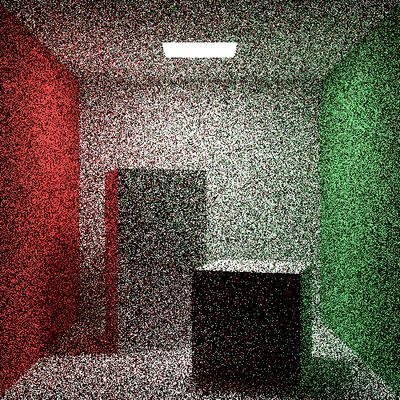
\includegraphics[width=\textwidth*\real{0.42}]{Images/noisy_image.jpeg}
	}
	\qquad
	\subfloat[Less noisy image]{
        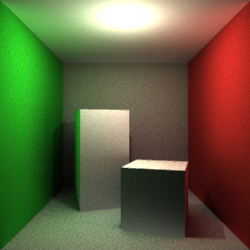
\includegraphics[width=\textwidth*\real{0.42}]{Images/less_noisy_image.png}
    }
	\caption{Noise in a ray traced image.}
    \label{fig:noise_example}
\end{figure}

Actually, in many ray tracing techniques, just one probe ray is cast, but the estimated light entering a point is temporally accumulated. This works because Monte-Carlo integration is unbiased.

\subsection{Variance Reduction Techniques}
In this section we will describe importance sampling, a variance reduction technique applicable to Monte-Carlo method to reduce the error of the estimate, without increasing the number of samples. This technique is particularly relevant in ray tracing, since we have a very limited number of probe rays we can cast. Eventually, we will show how importance sampling can be applied to the ray tracing context, and how its usage generates artifacts in the ray distribution in the rendered scene.

Variance reduction techniques, as the name suggests, are methods used in the Monte-Carlo context to reduce the variance of the estimator without increasing the computational effort.

One of the variance reduction techniques employed in ray tracing, and that is relevant to our work, is called Importance Sampling (IS). Let's imagine that we want to integrate a constant function. In this case, the positions where we place our samples are irrelevant: each time we run the Monte-Carlo simulation, the estimator will return the same result, therefore the variance is always 0.

The intuitive idea of importance sampling is to try to run the Monte-Carlo simulation always on a constant function. From a theoretical point of view, this is extremely easy: we simply need to divide the integrand $\textit{f}$ by a function proportional to it. Given the general Monte-Carlo estimator, this can be achieved by choosing a sampling PDF $p$ proportional to $\textit{f}$:

$$\langle F^N \rangle = \frac{1}{N}\cdot\sum_{i=0}^{N-1}\frac{\textit{f}(X_i)}{p(X_i)} \longrightarrow \frac{1}{N}\cdot\sum_{i=0}^{N-1}\frac{\textit{f}(X_i)}{k\cdot \textit{f}(X_i)}$$

From an operative point of view, with importance sampling it is more likely to get a sample from a portion where the integrand has a high value, but, at the same time, this sample will have a lower weight in the final estimate (because it is divided by a higher value). Whereas, if we get a sample from a portion where the integrand has low values, which is rare, its weight will be bigger. This means that the estimate comes from a finer-grained sampling of the portions where the integrand carries most of its information.

Even though from a mathematical point of view this is simple, from a concrete standpoint the technique can be difficult to apply. The main reason is that in many cases, such as in ray tracing, we don't have an analytical form of the integrand function, therefore finding a function proportional to it is problematic. Moreover, a bad choice of the PDF, can lead to an increase in the variance of the estimator, even compared to the uniform PDF.

Going back to the ray tracing context, the integrand function has this equation:

$$\int_\Omega BRDF(\bar{x}, \bar{\omega}_i, \bar{\omega}_o) \cdot \cos(\bar{n}, \bar{\omega}_i) \cdot L_i(\bar{x}, \bar{\omega}_i) d\bar{\omega}_i$$

It is possible to note that the function is made up of 3 terms: the $BRDF$, the geometry term and the incoming light term. We can therefore use a probability function proportional to one of the terms to reduce the variance:
\begin{description}
	\item[Cosine sampling] The sampling PDF is proportional to the geometry term of the rendering equation.
	\item[BRDF sampling] The sampling PDF is proportional to the BRDF. BRDFs can assume complex analytical forms, therefore sampling the BRDF is not always easy.
	\item[Light sampling] The sampling PDF should be proportional to the $L_i$ term of the rendering equation.
\end{description}

Light sampling is particularly problematic because we almost never have an analytical form of the $L_i$ function. The most used form of light sampling is called next event estimation (NEE), and is achieved by casting rays towards direct light sources. The way in which the light source to sample is chosen can be completely random or require complex strategies, such as in the case described in this article in the book \textit{Ray Tracing Gems}: \cite{multi_light_sampling}.

The main issue with next event estimation is that a direct light can be occluded by an object, or, conversely, a strong light could come from an indirect source, such as a reflection. For this reason, another technique, called path guiding \cite{path_guiding}, has been developed to consider mainly indirect lighting in the sampling PDF. Path guiding can be computationally expensive, therefore is often used in non-real-time scenarios, even though approximations have been proposed even for real-time ray tracing, such as \cite{real_time_path_guiding}.

\begin{figure}[H]
    \centering
    \subfloat[Next event estimation]{
        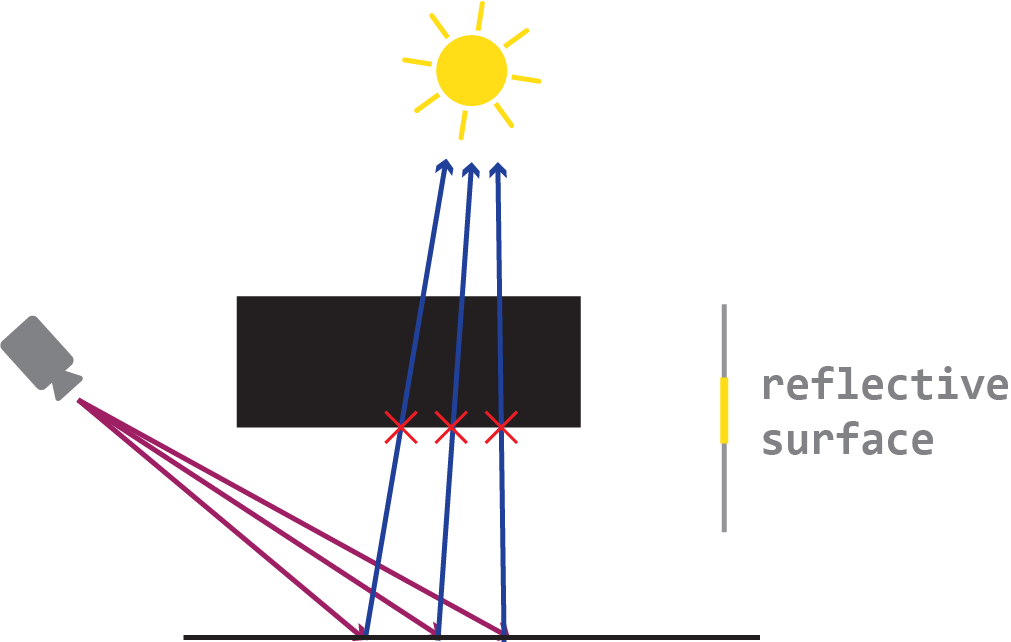
\includegraphics[width=\textwidth*\real{0.45}]{Images/nee.png}
	}
	\qquad
	\subfloat[Path guiding]{
        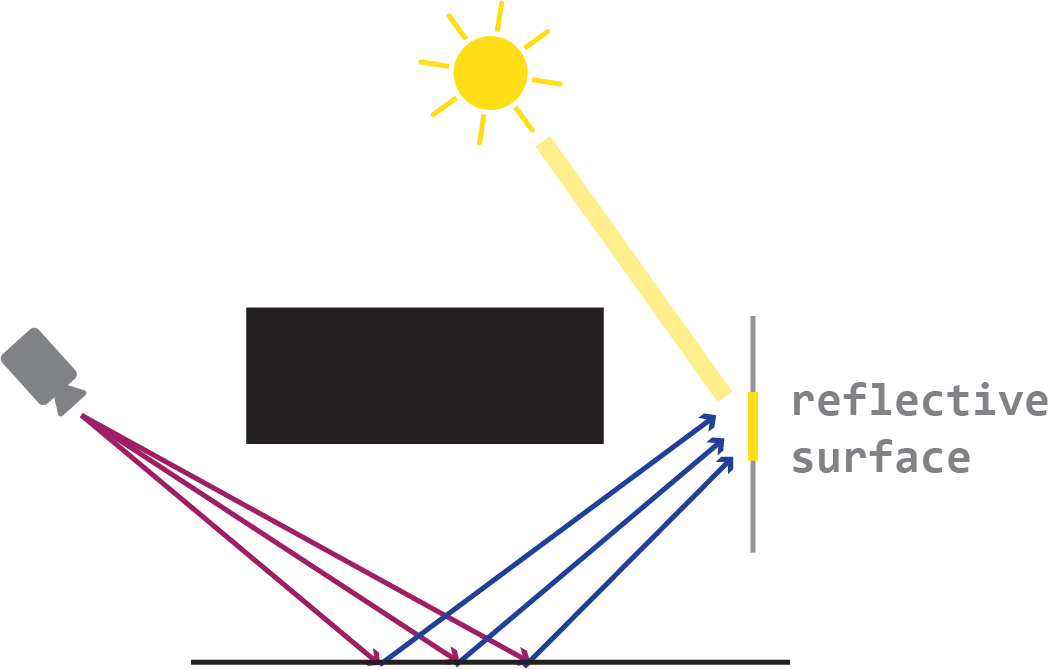
\includegraphics[width=\textwidth*\real{0.45}]{Images/path_guiding.png}
    }
	\caption{With NEE light is directly cast toward direct light sources. With path guiding, indirect illumination is taken into account in order to build a better sampling PDF, at a higher cost.}
    \label{fig:nee_and _path_guiding}
\end{figure}

Using BRDF sampling or light sampling in isolation as variance reduction PDFs can give better or worse results mainly based on the rendered section of the scene. For example, in a well illuminated scene with a mirror, using light sampling gives bad results. This happens because the BRDF of the mirror is null everywhere except for a spike in the perfect reflection direction. This means that its weight in the integrand is much more important than the weight of the $L_i$ term, which is almost constant being the scene well illuminated. If we use light sampling we will cast rays almost uniformly, and many of them will lose all of their energy as soon as they hit the mirror and reflect to a non-perfect-reflection direction.

On the contrary, in a scene with rough materials (such as concrete) and with few distant light sources, using light sampling would be beneficial, since many of the rays would be cast toward a light, instead of toward the void.

To remedy the problem of choosing the right importance sampling technique based on the portion of the scene, a new technique has been developed, called Multiple Importance Sampling (MIS) \cite{mis}.

The key take away from this section is that with importance sampling we use a non-uniform PDF to sample probe rays from. This creates artifacts in the ray distribution in the scene. In particular, if next event estimation is used, a big part of the rays will tend to go toward light sources. In chapter \ref{ch:projected_area_heuristic} we will study how these artifacts in the ray distribution can be exploited to design a faster technique to traverse a bounding volume hierarchy, which is the main subject of the next section \ref{sec:ray_tracing_acceleration_structures}.

\section{Ray Tracing Acceleration Structures} \label{sec:ray_tracing_acceleration_structures}
In this section we will describe the first family of software optimizations we talked about in section \ref{ssec:optimizations_overview}. These optimizations aim at reducing the time needed to find the intersections between a ray and the geometry of the scene. Usually this is achieved by organizing the scene geometry in a spatial data structure, or by wisely choosing the order in which rays are cast, in order to improve the spatial coherency of the data accesses on the GPU \cite{ray_coherency}. After a brief description of older acceleration structures, we will focus on the state-of-the-art acceleration data structure, called Bounding Volume Hierarchy (BVH), and present how it is constructed. We will eventually show the assumptions on which the construction algorithm is based, whose refutation will be the main subject of the novel approach we propose in the next chapter \ref{ch:projected_area_heuristic}.

\subsection{The Need for Acceleration Structures} \label{ssec:need_for_acceleration_structures}
As we've seen throughout this chapter, in any of the algorithms of the ray tracing family, casting rays is the core of the procedure. Rays are primarily cast from the camera toward the scene, and subsequently, based on the specific algorithm used, they hit objects and bounce off of them. Until now, however, we have overlooked how, in a concrete scenario, the algorithm can detect what is the object hit by the ray. 

Before delving into the algorithms that can be used to carry out this task, it is important to understand how an object is described in the world of computer graphics. In the history of computer graphics a lot of techniques to represent an object have been developed. Some examples are volumetric rendering with voxels \cite{voxel_rendering}, signed distance fields \cite{sdf} and implicit functions that work best with the ray marching algorithm \cite{ray_marching}, or point clouds. By the way, the most common method to represent 3D objects are polygonal meshes.

A polygonal mesh describes an object by defining its surface via points, edges and faces (usually triangles). Meshes's success derived from the fact that they were one of the first representations proposed in the world of computer graphics. This led to a big part of the research converging to this specific representation form. For example, GPUs are specialized for the rendering of triangular meshes via rasterization, even though in the last few years their architecture has been made more flexible.

\begin{figure}[H]
    \centering
    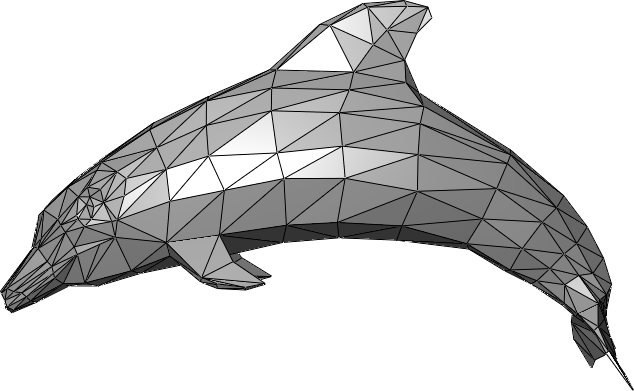
\includegraphics[width=\textwidth*\real{0.5}]{Images/triangular_mesh.png}
    \caption{A triangular mesh.}
    \label{fig:triangular_mesh}
\end{figure}

Meshes are also handy to create for graphic artists, and can be easily modeled to represent many kinds of objects, even though they are not suited to represent liquids or gases, such as clouds. Meshes, since they describe only the outside surface of an object, can prove difficult to use in applications where the interior is important, such as medical visualizations or games where objects can be dynamically destroyed. In these contexts it is usually preferred to employ voxels. Moreover meshes are a discrete representation, meaning that, once created, they cannot be used to visualize the details of the object at an arbitrary resolution, contrary to implicit functions. However, techniques to change the resolution based on the dynamic situation have been developed, such as LODing, tessellation \cite{tessellation} or more recent methods such as Nanite \cite{nanite}.

Regardless of their advantages and disadvantages, triangular meshes are by far the most used representation, therefore in this work we decided to focus on them in the scenario where the rendering technique is an algorithm of the ray tracing family.

In order to find the intersection between a ray and a list of meshes making up a scene, we need to test the intersections between the ray and all the triangles making up the meshes, and keep the closest one\footnote{In some scenarios, such as when we just want to check for occlusion, it is not necessary to find the closest intersection, but just to find an intersection. In this case some optimizations can be developed, but the core concepts remain the same.}.

The naive way of detecting the intersection is the brute-force solution of iterating over all of the triangles and storing the closest intersection found so far. The algorithm we used to detect the intersection between a ray and a triangle in our implementation can be found in appendix \ref{sec:ray_triangle_intersection}. Despite working, this method cannot be practically used either in real-time scenarios, nor in non-real-time ones. The problem resides in the fact that there are too many triangles to test against. Even in a non-real-time case this approach would be too expensive. Indeed, even if the time budget for a frame is big, meshes created for non-real-time purposes usually have a way higher triangle resolution, and also way more rays to trace. From a complexity point of view, tracing a scene with $n$ triangles and $m$ rays in this way has complexity $\mathcal{O}(m\cdot n)$.

This is the reason why acceleration structures have been developed. Most of the acceleration structures organize the triangles in a hierarchical fashion, so that it is possible to exclude a big chunk of them if a ray doesn't hit certain parts of the scene. One very simple example of acceleration structure would be to divide the scene into 2 parts and keep track of what triangles reside on each one. Now, if a ray doesn't hit one of the 2 parts, it is possible to exclude all of the triangles contained in that region, without having to test them one by one.

Acceleration structures can be divided into 2 categories:
\begin{description}
	\item[Space partitioning] The space is recursively subdivided into disjoint regions. Objects (triangles) can potentially appear in more than one region, if they are overlapping. 
	\item[Object partitioning] Objects are subdivided into disjoint sets, enclosed into spatial regions. The regions can potentially be overlapping.  
\end{description}

Historically, initially the first family of acceleration structures has been used, but todays state-of-the-art acceleration structure is the BVH, part of the second family. We will now very briefly list some of the most famous acceleration structures historically used for ray tracing, and, in the next section, we'll diffusely talk about the BVH.

The first space partitioning acceleration structure developed is the uniform grid. In this structure the 3-dimensional space of the scene is subdivided into static fixed-sized cells in a regular pattern. Then, each triangle is assigned to all the cells it at least partially covers. This can be at least a single cell, to, potentially all the cells of the scene. When a ray is traced, first, a cell it intersects is found, and then, all the triangles inside this cell are tested against the ray. This is repeated for all the cells the ray hits in its path. If an intersection $P$ is found, then, all the cells that are at a further distance from the ray origin than $P$ can be discarded without testing individual triangles.

\begin{figure}[H]
    \centering
    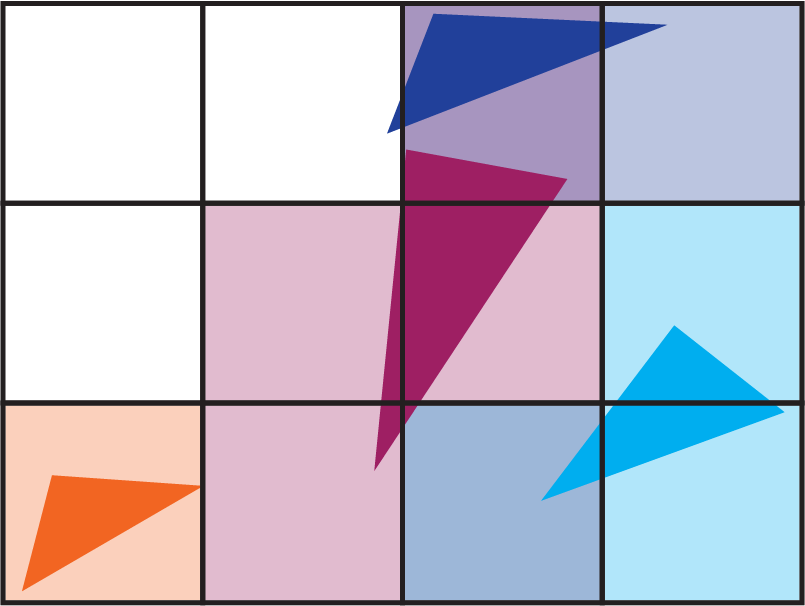
\includegraphics[width=\textwidth*\real{0.45}]{Images/uniform_grid.png}
    \caption{The uniform grid in 2D.}
    \label{fig:uniform_grid}
\end{figure}

The uniform grid, while being an improvement over the brute-force approach, still lacks adaptability. Based on how the scene is composed, it is possible for some cells to be empty and others overcrowded. Moreover, as in any space partitioning data structure, it is possible that a triangle is tested more than once if it overlaps more than one cell. This could be avoided by using some intersection caching techniques, such as mailboxing \cite{mailboxing}.

In order to solve the adaptability problem of the uniform grid, octrees started being used. An octree is another 3D spatial data structure, and it is a tree where each node has 8 children. To subdivide a node into 8 children, it is divided by 3 planes, one perpendicular to each dimension, passing from the center of the parent node. This process is recursively executed until a specified amount of objects (triangles) remains inside a single node, or until the depth of the tree gets past a threshold. Since the octree is a complete tree, and the size and center of each child can be automatically computed starting from the size of the root and the level\footnote{$size_{children} = size_{root} / 2^{level}$ given that the root has level $0$.}, it is possible to store the octree in an implicit array structure, making it more efficient both from an access pattern and space point of view.

\begin{figure}[H]
    \centering
    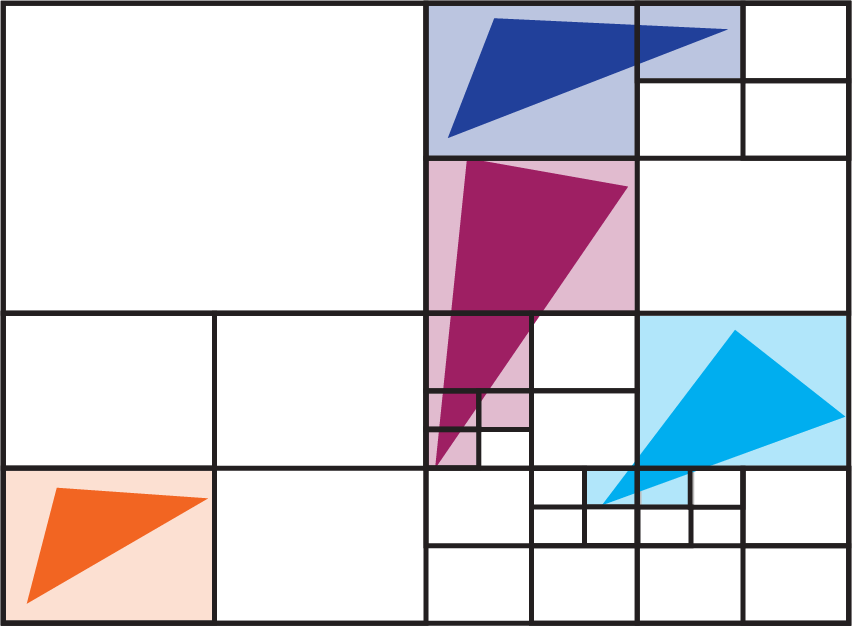
\includegraphics[width=\textwidth*\real{0.45}]{Images/quadtree.png}
    \caption{A 2D octree (quadtree).}
    \label{fig:octree}
\end{figure}

It is important to note how octrees adapt better to the scene. Indeed, compared to fixed grids, they alleviate the \textit{teapot in the stadium} problem, namely the issue that appears when there is a scene with different densities of objects. For example, precisely what happens when we have a small but high-resolution object (a teapot), inside a big and mostly empty space (a stadium). With octrees this problem is handled by having few big and empty cells in the regions where there is a low density of triangles, and many small cells where there are high-resolution objects. In this way less memory is wasted, and even traversal is improved. Indeed, if a ray passes through empty space, just few cells must be checked, instead of a bigger amount as in the case of a uniform structure like the fixed grid. Conversely, in case a ray goes through a dense region, fewer triangle tests will be carried out, because the cells the ray intersects are smaller and not overcrowded. Another advantage of octrees is that they are a tree data structure. This implies that if a node is not hit by a ray, all its children can be immediately discarded.

\begin{figure}[H]
    \centering
    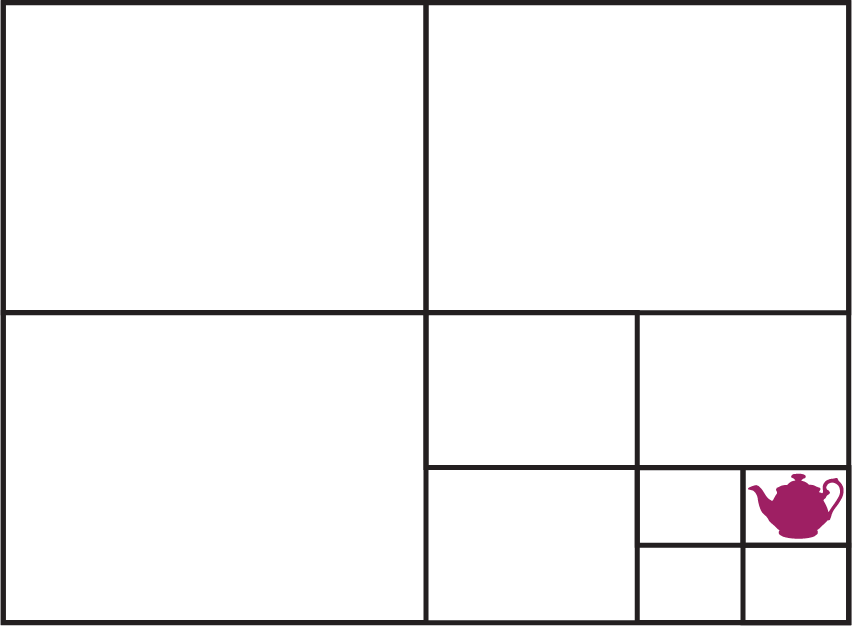
\includegraphics[width=\textwidth*\real{0.45}]{Images/teapot_stadium.png}
    \caption{How an octree adapts to a \textit{teapot in the stadium} kind of scene.}
    \label{fig:octree_teapot_stadium}
\end{figure}

Another structure that is a generalization of octrees and delivers similar performance is the kd-tree. In 3D kd-trees each node is split into 2 children by a plane. At each level the plane is perpendicular to one of the dimensions, in a round-robin fashion (for example, at level 0 it is normal to $x$, at level 1 to $y$, at level 2 to $z$ and so on). Differently from octrees, the plane doesn't necessarily have to pass through the center of the parent node, making their construction even more flexible.

\begin{figure}[H]
    \centering
    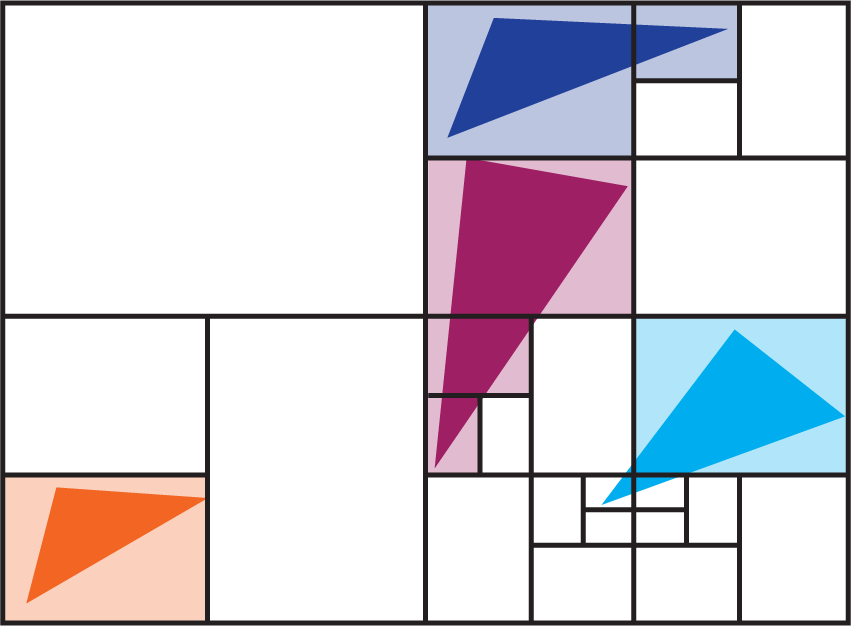
\includegraphics[width=\textwidth*\real{0.45}]{Images/kd_tree.png}
    \caption{A kd-tree in 2D.}
    \label{fig:kd_tree}
\end{figure}

These are the most prominent spatial data structures used for ray tracing. However, nowadays an object partition structure is used, called bounding volume hierarchy, which we will analyze in the next section.

\subsection{The Bounding Volume Hierarchy} \label{ssec:the_bounding_volume_hierarchy}
A BVH \cite{bvh_primer} is a binary tree\footnote{Technically it can be a tree with any breadth, but binary trees are the most common ones.} where each node wraps some of the triangles in the scene in a bounding volume. Given a node $A$ wrapping the triangles in the set $T_A$, then the two children of $A$, called $B$ and $C$, wrap the triangles in the sets $T_B$ and $T_C$ such that $T_B \cup T_C = T_A$. Thanks to this structure, if a ray doesn't intersect a bounding volume, we deduce that it will not intersect any of the triangles contained in the bounding volume too, making it possible to discard them without having to perform any additional intersection test.

Assuming the best-case scenario where a ray always hits only one of the 2 children of a given node during traversal, if the BVH is balanced and has one triangle per leaf, then the complexity of finding an intersection between a ray and the scene is $\mathcal{O}(log_2(n))$, where $n$ is the number of triangles. This is not always the case, since it often happens that a ray hits both the children of a given node. One of the heuristics that we propose in this thesis in chapter \ref{ch:splitting_plane_facing_technique}, aims at reducing the number of this expensive situation, by building the BVH in a smart way.

The bounding volume in which a BVH encloses triangles should have a form that is cheap to intersect with a ray, and also cheap to build given a set of triangles.

A choice can be a sphere, which is easy to test against a ray. Moreover, building the tightest enclosing sphere given a set of triangles is as simple as finding the 2 triangles furthest away in each direction, computing the middle point and setting as radius the distance between the furthest triangle and the middle point. The negative aspect of using bounding spheres lies in the fact that a sphere extends equally in all directions in 3D space. This means that if the triangles are displaced in a way where they extend more in one direction than in other ones, the bounding sphere will present a lot of slack space, and won't enclose the triangles tightly. This is not ideal, because in the traversal phase a non-tight bounding volume generates a lot of false positives, namely situations where the bounding volume is hit but no triangle is intersected.

\begin{figure}[H]
    \centering
    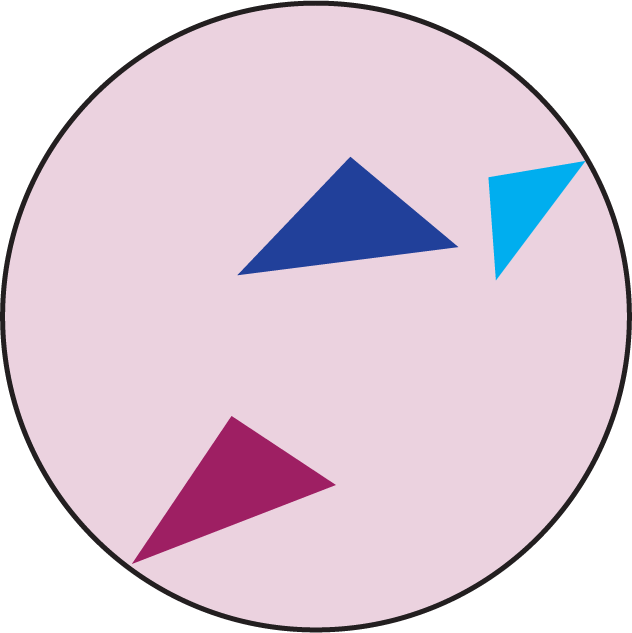
\includegraphics[width=\textwidth*\real{0.25}]{Images/bounding_sphere_slack.png}
    \caption{Bounding circle (2D bounding sphere) can present large slack spaces.}
    \label{fig:bounding_sphere}
\end{figure}

At the opposite side of the spectrum there are polygonal bounding volumes. In this case they are able to tightly enclose the triangles, but building them is not easy, and intersecting them can prove as expensive as intersecting the set of triangles itself.

Another option is using Oriented Bounding Boxes (OBB). Oriented bounding boxes in 3D are rectangle parallelepiped. This means that they can have a different extension in 3 different arbitrary directions (each one perpendicular to the remaining two), making them better at tightly enclosing any distribution of triangles compared to spheres. However, computing a tightly enclosing OBB starting from the set of triangles involves using the principal component analysis \cite{obb_construction}, which can be too expensive in real-time scenarios. Moreover, intersecting a ray against an OBB involves a rotation transformation, which, again, can be too slow, especially during the traversal phase. In general OBBs are too slow in many scenarios, but, given their ability to tightly enclose triangles, can be used along with AABBs \cite{obbs_for_bvhs}.

\begin{figure}[H]
    \centering
    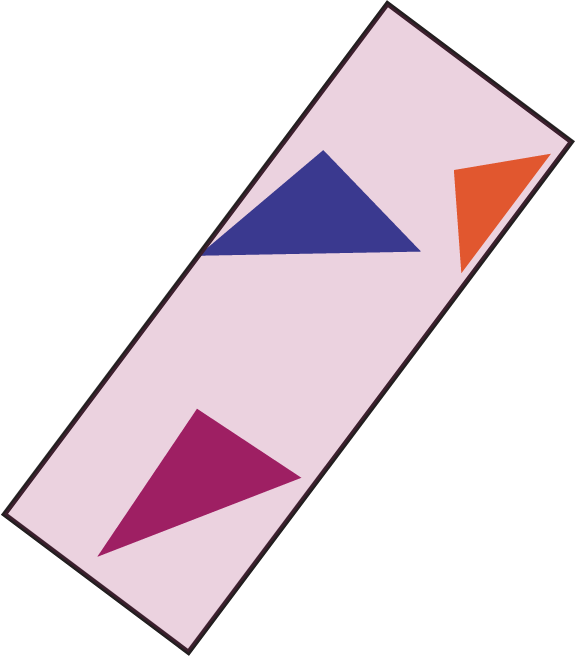
\includegraphics[width=\textwidth*\real{0.3}]{Images/obb_slack.png}
    \caption{A 2D OBB.}
    \label{fig:obb}
\end{figure}

Axis-Aligned Bounding Boxes (AABB) are the most used bounding volumes. AABBs are OBBs that have no rotation, and are always aligned with the cartesian axes. This means that AABBs can indeed have a different extension in 3 directions, but the directions are limited to the ones of the cartesian axes. These limitations make them worse at tightly enclosing triangles than OBBs, but at the same time make it way easier to build them and intersect them with a ray. To build an AABB starting from a set of triangles, it suffices to iterate over all the triangles and keep track of the minimum and maximum point in all 3 dimensions. An AABB is then fully described by its minimum and maximum point. The algorithm to test whether a ray intersects an AABB is fast and can be implemented in a GPU-friendly branchless way, as described in appendix \ref{sec:ray_box_intersection}.

\begin{figure}[H]
    \centering
    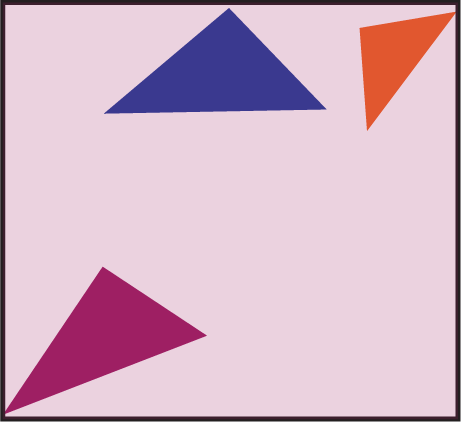
\includegraphics[width=\textwidth*\real{0.25}]{Images/aabb_slack.png}
    \caption{A 2D AABB.}
    \label{fig:aabb}
\end{figure}

AABBs are the most used bounding volumes both in real-time and non-real-time ray tracing. For this reason, from now on, when we refer to a BVH we will always consider the case of a BVH based on AABBs.

\begin{figure}[H]
    \centering
    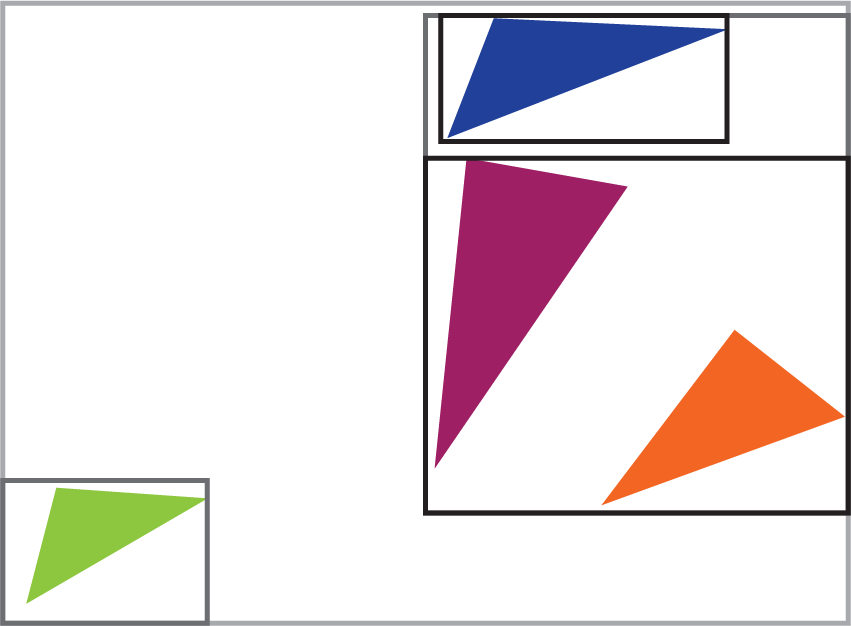
\includegraphics[width=\textwidth*\real{0.45}]{Images/bvh_2d.png}
    \caption{A 2-dimensional BVH.}
    \label{fig:bvh_2d}
\end{figure}

Despite it is not clear that BVHs' raw performance is better than kd-trees', especially on large scenes \cite{bvh_vs_kd_tree}, they became the state-of-the-art acceleration structure for many practical reasons.

First of all, being an object partitioning data structure, they can solve the \textit{teapot in a stadium} problem even better than kd-trees. This is because it is possible to completely cut off empty space, as it is possible to observe in figure \ref{fig:bvh_2d}.

Moreover, and this is especially relevant in a dynamic real-time scenario such as a videogame, BVHs are easier to update when the geometry of the scene changes \cite{bvh_update}.

BVHs construction algorithm is also simpler than kd-trees', allowing a faster build-time, which can be crucial in highly dynamic real-time applications. And they also have a smaller memory footprint compared to kd-trees, as mentioned in \cite{bvh_spatial_splitting} and \cite{bvh_advantages}.

\subsection{BVH Construction} \label{ssec:bvh_construction}
Building the optimal BVH according to some metric is an NP-complete problem. In order to do so, the algorithm would have to build all the possible BVHs given a set of triangles, compute the metric and keep the best one. The number of possible different binary trees grows factorially with the number of leaves. Given $n$ leaves, the number of possible binary trees is the $n-1$ Catalan number \cite{catalan_numbers}: $C_{n} = \frac{(2n)!}{(n+1)! \cdot n!}$. The number of possible BVHs is even bigger, because, since a leaf can contain more than one triangle, it is not a given that the number of leaves corresponds to the number of triangles.

Given that building the optimal BVH is not feasible even in a non-real-time scenario, research started studying methods to build a BVH with an acceptable quality faster. This resulted in the use of greedy algorithms and heuristics.

The base algorithm fo building a BVH can be summarized in these steps:
\begin{algorithm}[H]
	\caption{Summarized BVH construction algorithm.}
	\begin{algorithmic}[1]
		\Function{BuildBvh}{$triangles$}
		\Let{$leftNode$}{[\;]}
		\Let{$rightNode$}{[\;]}
		\Let{$cost$}{$\infty$}
		\Loop{$\;cost < threshold \AOr all\;possible\;splits\;attempted$}
			\Let{$[leftNodeTmp, rightNodeTmp]$}{$SplitTriangles(triangles, howToSplit)$}
			\Let{$costTmp$}{$ComputeCost(leftNodeTmp, rightNodeTmp)$}
			\If{$costTmp < cost$}
				\Let{$leftNode$}{$leftNodeTmp$}
				\Let{$rightNode$}{$rightNodeTmp$}
				\Let{$cost$}{$costTmp$}
			\EndIf
		\EndLoop
		\If{$\ANot StopCriterion(cost, leftNode, rightNode)$}
			\State{$BuildBvh(leftNode.triangles)$}
			\State{$BuildBvh(rightNode.triangles)$}
		\EndIf
		\EndFunction
	\end{algorithmic}
	\label{alg:bvh_construction_summary}
\end{algorithm} 

The proposed algorithm is a greedy one. This means that it tries to minimize the cost function locally, at each level of the BVH, but when a decision is taken, it is not possible to change it. Making the local optimal choice doesn't imply that the global minimum of the cost function will be found, but at least it makes the problem tractable.

The algorithm can be divided into 3 steps: triangles splitting, cost computation and stopping criterion.

\subsubsection*{Stopping Criterion}
The stopping criterion phase decides whether the $BuildBvh$ function should make the recursive call and split the new children nodes. The stopping criterion can be based on different metrics, among which:
\begin{itemize}
	\item Children cost
	\item Total triangles in children
	\item BVH level
\end{itemize}

\subsubsection*{Triangles Splitting} \label{ssec:triangles_splitting}
Given the set of triangles of the parent node, in this phase the algorithm tries to split them into two subsets and build the enclosing bounding volumes.

In order to split the triangles into two subsets, a plane is chosen, and based on which side of the plane the barycenter of each triangle is, the triangle is assigned to one of the two subsets. This means that it is possible that a triangle has some vertices in the opposite half-space compared to the one it has been assigned to. This is one of the reasons why two children can have some of their volumes overlapping. 

\begin{figure}[H]
    \centering
    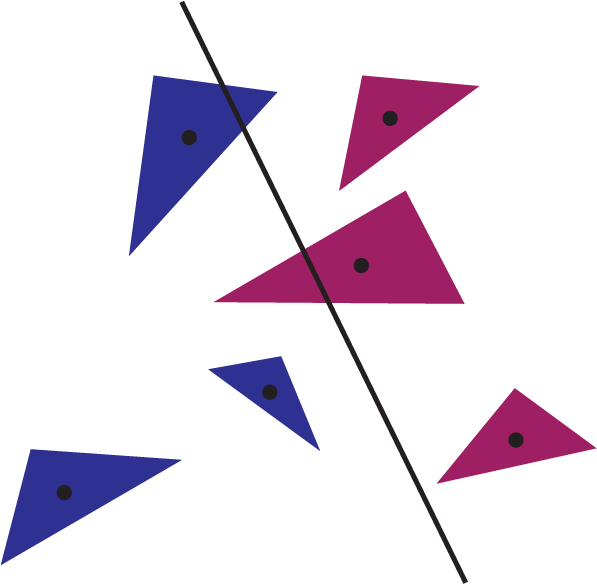
\includegraphics[width=\textwidth*\real{0.4}]{Images/triangle_splitting_arbitrary.png}
    \caption{Triangles splitting via arbitrary plane.}
    \label{fig:triangles_splitting}
\end{figure}

As shown by \cite{bvh_overlapping_metric} too much overlapping between children nodes leads to a decrease in the quality of the final BVH. For this reason, in chapter \ref{ch:splitting_plane_facing_technique} we propose a novel technique trying to take into account the overlapping during this phase of BVH construction.

In order to choose which plane to use to split the triangles, some optimizations can be employed. In BVHs based on AABBs it is useful to try to split the triangles only in the 3 cartesian directions. Usually just one of the directions is chosen, in order to further optimize the process. The way in which the direction is chosen can vary based on the methods used. An often employed technique is to cut along the longest dimension of the parent AABB. Another one is to cut in a round-robin fashion, similar to what is done in kd-trees. In chapter \ref{ch:splitting_plane_facing_technique} we propose a novel method, as mentioned above.

Another advantage of using only the 3 cartesian directions is that, in order to detect the half-space a point falls into, it is sufficient to compare one of its coordinates with the coordinates of a point the plane is passing through. This is an optimization compared to computing the cross-product, like in the case where the plane has an arbitrary normal direction.

After choosing a splitting direction, all possible cuts in that direction should be tested. Given an amount on $n$ triangles to be split, trying all the possible cuts in one direction means trying $n-1$ subdivisions, where the splitting plane is placed each time on the barycenter of a triangle. Since $n$ can be a big number, especially while running the algorithm on the first levels of the BVH, where nodes are big, a technique called binning can be introduced.

With binning, instead of trying every possible cut, a predefined number of cuts is attempted. The splitting plane is translated each time by a fixed length (a bin) along the chosen cutting direction from the position of the previous cut. By using binning it is possible to miss some of the possible cuts, especially in a region dense of triangles. However, the most relevant cuts are often positioned where there is a big gap in one direction between two consecutive triangles. This is because it is possible to leverage the big gap to cut off as much space as possible. Whereas, if the gap is small, it is likely that the resulting children nodes' AABBs overlap. For this reason binning is an efficient approximation, especially in the higher levels of the BVH.

\begin{figure}[H]
    \centering
    \subfloat[Triangles splitting without binning]{
        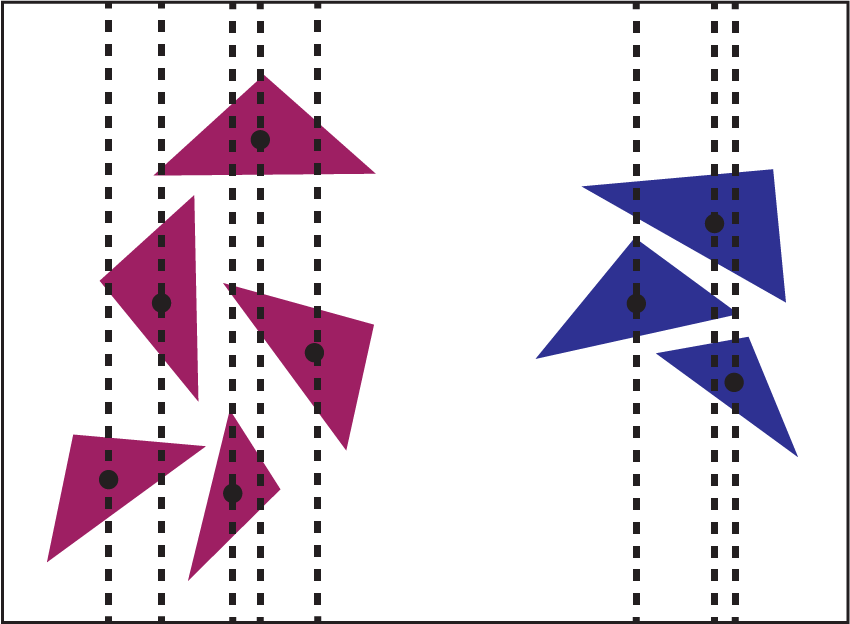
\includegraphics[width=\textwidth*\real{0.45}]{Images/split_no_binning.png}
	}
	\qquad
	\subfloat[Triangles splitting with binning]{
        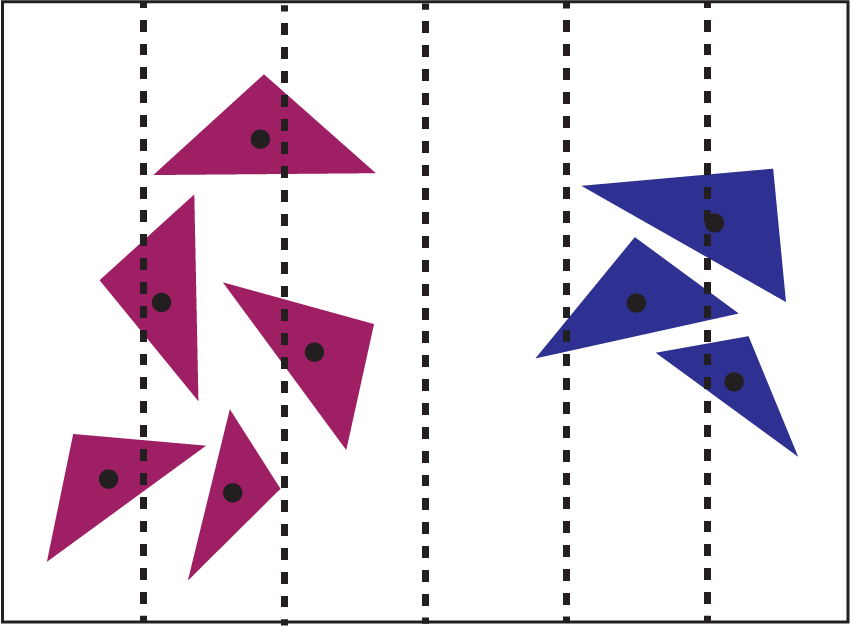
\includegraphics[width=\textwidth*\real{0.45}]{Images/split_binning.png}
    }
	\caption{With binning it is possible to lose some cuts, but the most relevant ones are always found, for example the cut dividing the blue and purple triangles.}
    \label{fig:triangles_splitting_binning}
\end{figure}

After generating the two subsets of triangles, the enclosing AABBs must be built. The process to build an AABB from a set of triangles is straight-forward, and is summarized by this algorithm:
\begin{algorithm}[H]
	\caption{AABB building from triangles set.}
	\begin{algorithmic}[1]
		\Function{BuildAabb}{$triangles$}
		\Let{$min$}{$(\infty,\infty,\infty)$}
		\Let{$max$}{$(-\infty,-\infty,-\infty)$}
		\ForAll{$t \in triangles$}
			\Comment{$t.v_k$ is the $k^{th}$ vertex of the triangle $t$}
			\Let{$min.x$}{$Min(min.x, t.v_0.x, t.v_1, t.v_2.x)$}
			\Let{$max.x$}{$Max(max.x, t.v_0.x, t.v_1, t.v_2.x)$}
			\Let{$min.y$}{$Min(min.y, t.v_0.y, t.v_1, t.v_2.y)$}
			\Let{$max.y$}{$Max(max.y, t.v_0.y, t.v_1, t.v_2.y)$}
			\Let{$min.z$}{$Min(min.z, t.v_0.z, t.v_1, t.v_2.z)$}
			\Let{$max.z$}{$Max(max.z, t.v_0.z, t.v_1, t.v_2.z)$}
		\EndFor
		\State \Return $Aabb(min, max)$
		\EndFunction
	\end{algorithmic}
	\label{alg:aabb_creation}
\end{algorithm} 

\subsubsection{Cost Computation - Surface Area Heuristic} \label{ssec:cost_computation}
In the previous section we have described how a standard BVH construction algorithm can split the triangles of a node into two subsets, and compute the AABB for each one of them. In this section we will analyze how the algorithm decides whether a split is better than another one.

To choose the best split, a BVH construction algorithm sorts the splits proposed by the splitting triangles phase, by assigning to each one a value through a cost function. 

The aim of a cost function is to accurately predict how \textit{good} the final BVH will be. The concept of \textit{goodness} or \textit{quality} of a BVH is directly related to how fast an arbitrary ray is able to traverse it to find the first intersection with a triangle. It is possible to evaluate the cost function for every node as if it was a leaf node, and this is useful while building the BVH with the greedy algorithm. It is also possible to compute the cost function of the overall BVH, which is used to evaluate the quality of the BVH built.

The most used cost function is called Surface Area Heuristic (SAH) \cite{sah}, and is based on a very simple idea: the smaller the surface area of a node's AABB, the less likely is for this node to be hit by a ray. If a node is hit less times by a ray, it means that fewer checks are needed to traverse the BVH, therefore its quality, as we defined it above, is higher.

Given an AABB, it is trivial to compute its surface area as: 
$$A=(max_x-min_x)\cdot (max_y-min_y) + (max_x-min_x)\cdot (max_z-min_z) + (max_y-min_y)\cdot (max_z-min_z)$$

Now, we would like to have a cost function that is agnostic to the absolute size of the scene. For this reason, instead of using directly the surface area to compute the cost metric, we transform it into the probability that a ray hits a specific node.

To do so SAH makes some reasonable assumptions on some properties of the rays in the scene:
\begin{itemize}
	\item A ray always hits the AABB enclosing the whole scene;
	\item All rays have origin outside the AABB enclosing the whole scene, and their positions are uniformly distributed;
	\item Rays never intersect any primitive, and are infinitely long;
	\item Rays are uniformly distributed in their direction space.
\end{itemize}

With these assumptions in place, which we'll analyze better in section \ref{sec:sah_hypotheses_fall}, we can define the probability a ray hits a node $K$ as:
$$p(ray\; hits\; K) = \frac{Area_K}{Area_{root}}$$

Since all rays hit the root AABB, we can interpret it as the certain event. And since the rays' directions are uniformly distributed, the surface area can be mathematically interpreted as a measure of how likely it is for a ray to hit an AABB.

\begin{figure}[H]
    \centering
    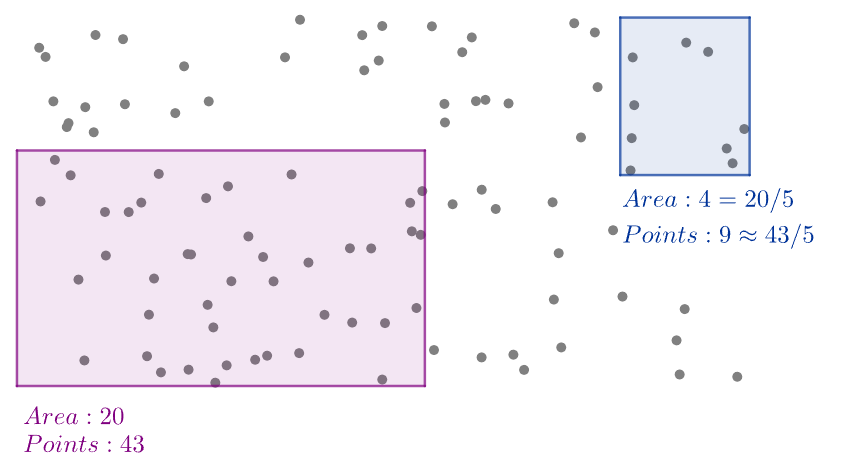
\includegraphics[width=\textwidth*\real{0.7}]{Images/area_prob_visualization.png}
    \caption{Visual relationship between AABB area and hit probability in 2D, under the assumption rays are uniformly distributed.}
    \label{fig:area_probability_visual}
\end{figure}

Finally, in order to compute the cost function, we have to also take into account the cost of the intersection test between a ray and a triangle, and a ray and an AABB. In literature a cost of $1.2$ is assigned to the first test, and a cost of $1$ to the second one.

We now have all the elements to define the SAH cost function for a node $K$:
$$Cost_{SAH}(K) = \frac{Area_K}{Area_{root}} \cdot \#triangles_K \cdot 1.2$$

The $\#triangles_K \cdot 1.2$ part tells us that when this node is hit by a ray, a ray-intersection test per triangle must be carried out. The term $\frac{Area_K}{Area_{root}}$ weights the cost of computing the ray-intersection tests with the probability that this node is actually hit. This means that, even if a node has a lot of triangles in it, if these triangles are all packed in a small region, the cost of the node will not be too high, because it is unlikely for a ray to hit the node in the first place.

It is important to note that this formula returns the cost of a node in isolation. But the nodes we are dealing with are part of a BVH. In other words, when an internal node of a BVH is hit, this doesn't trigger a ray-triangle test for all of its triangles (as suggested by the formula), but only recursively triggers ray-AABB tests against its two children. Only when this formula is used on leaf nodes, the returned cost actually reflects the real cost of a ray intersecting the node.

Therefore why are we suggesting to use this formula? The answer is that we are building the BVH with a greedy algorithm. When we have to evaluate a node, we have no way of knowing how its children will be, therefore the only way is to estimate its cost as if it didn't have any children at all, as if it was a leaf node.

However it is also useful to have a way to evaluate the cost of a BVH a-posteriori. In this case, based on the node type, we can have two situations:
\begin{description}
	\item[Leaf node] The cost of a leaf node can be computed with the same formula we have analyzed, for the reasons we have stated above.
	\item[Internal node] When an internal node is hit, the next step of the traversal is to perform a ray-AABB test with each one of the two children. Therefore the cost is: $Cost_{SAH}(K_{intern}) = \frac{Area_K}{Area_{root}} \cdot 2 \cdot 1$. 
\end{description}

By merging the formulae to compute the cost of leaf and internal nodes, the cost function of a BVH assumes this form:
$$Cost_{SAH}(BVH) = \sum_{L \in leaf\; nodes} \frac{Area_L}{Area_{root}} \cdot \#triangles_L \cdot 1.2 + \sum_{I \in internal\; nodes} \frac{Area_I}{Area_{root}} \cdot 2 \cdot 1$$

\chapter{Projected Area Heuristic} \label{ch:projected_area_heuristic}
In chapter \ref{ch:background_theory} we described how ray tracing works. In particular, in section \ref{sec:monte_carlo_and_variance_reduction_techniques} we have seen how importance sampling generates artifacts in the ray distribution of the scene. In section \ref{sec:ray_tracing_acceleration_structures} we described how it is possible to build an acceleration structure to speed up the ray-scene intersection process, and we have shown how the surface area heuristic is the state-of-the-art method to build high-quality BVHs. In this chapter, we will show that some of the hypotheses of the SAH are not satisfied in a real-world scenario, due to the use of importance sampling. We will eventually propose a new heuristic, called Projected Area Heuristic (PAH), and show the situations where it can be used to build BVHs. In this chapter we will describe the problem and the solutions from a theoretical point of view; all the implementation details will be thoroughly discussed in chapter \ref{ch:implementation}.

\section{SAH Hypotheses Fall} \label{sec:sah_hypotheses_fall}
In section \ref{sec:ray_tracing_acceleration_structures} we have seen that the surface area heuristic, used to build high-quality BVHs with the described greedy algorithm, works under these hypotheses:
\begin{itemize}
	\item A ray always hits the AABB enclosing the whole scene;
	\item All rays have origin outside the AABB enclosing the whole scene, and their positions are uniformly distributed;
	\item Rays never intersect any primitive, and are infinitely long;
	\item Rays are uniformly distributed in their direction space.
\end{itemize}

In a standard situation, the first hypothesis can be considered true for all the rays. It is still possible, in some scenarios, that a part of the rays doesn't hit the scene. Examples can be found in the discussion on the test cases for our thesis in chapter \ref{ch:experimental_results}, however, in most scenarios, all the rays hit the scene, because casting a ray away from the scene would be wasteful.

For what concerns the second hypothesis, the situation is completely different. Indeed, in many applications the camera is inside the scene, therefore the rays' origin is inside the scene too. But even in a situation where the camera is placed outside the scene, still the majority of rays would have origin inside. This happens because in many algorithms of the ray tracing family, the primary rays (rays cast from the camera position) are in a much smaller number than the secondary rays. With secondary rays we refer to what we called in the previous chapter \textit{probe rays}, namely those rays originating after a ray-triangle intersection. As we have seen, generating probe rays to evaluate the rendering equation is a recursive process, and in order to obtain an image with an acceptable amount of noise, a lot of probe rays must be cast.

Studies about this issue with the surface area heuristic have been carried out. For example, in this article \cite{sah_interior_rays}, Fabianowski et al. divide the scene into discrete regions, and try to evaluate the hit probabilities from the center of each one.

The third and fourth hypotheses have both to do with how the rays are distributed in the 3D space of the scene. It is easy to see how the third hypothesis doesn't hold true in a real-world scenario. Of course primitives will block rays, thus potentially creating regions of the scene where few or no rays are present (imagine the region of space inside an opaque box, or even more in general, the space inside the boundaries of meshes). 

For what concerns the last hypothesis, we have to remember how Monte-Carlo integration works. In theory, after a ray hits an object, there is an equal probability it bounces toward any direction in the hemisphere. This behavior, considering that the other hypotheses hold true, would create a uniform distribution of rays in the scene. However, as we have seen in section \ref{sec:monte_carlo_and_variance_reduction_techniques}, importance sampling makes it so that the probe rays distribution is not uniform. In particular, if direct light sampling is used, a lot of probe rays will tend to go toward light sources. This artifact in the ray distribution shows how not even the last SAH hypothesis holds true.

\begin{figure}[H]
    \centering
	\subfloat[Without importance sampling]{
    	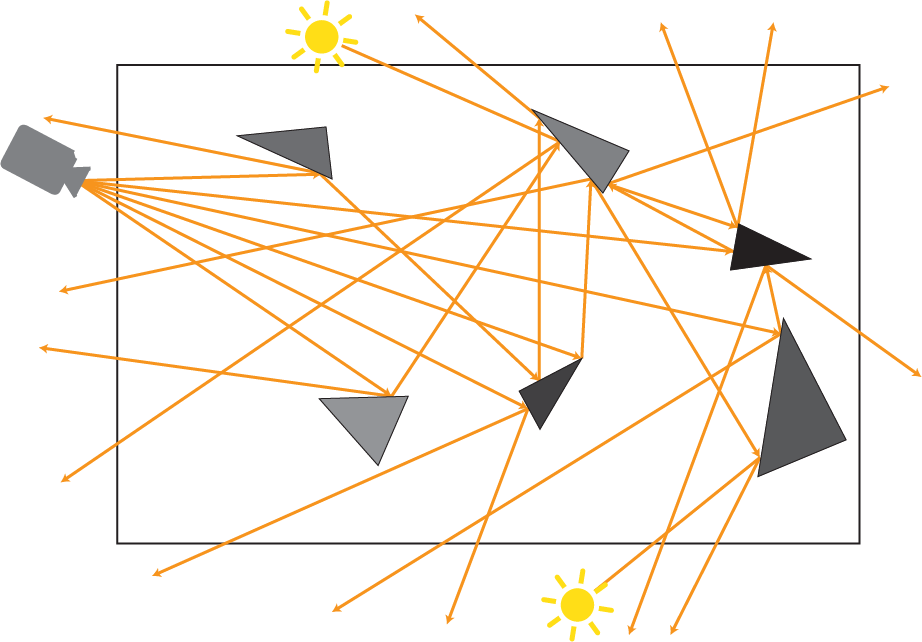
\includegraphics[width=\textwidth*\real{0.45}]{Images/without_importance_sampling.png}
	}
	\qquad
	\subfloat[With importance sampling]{
    	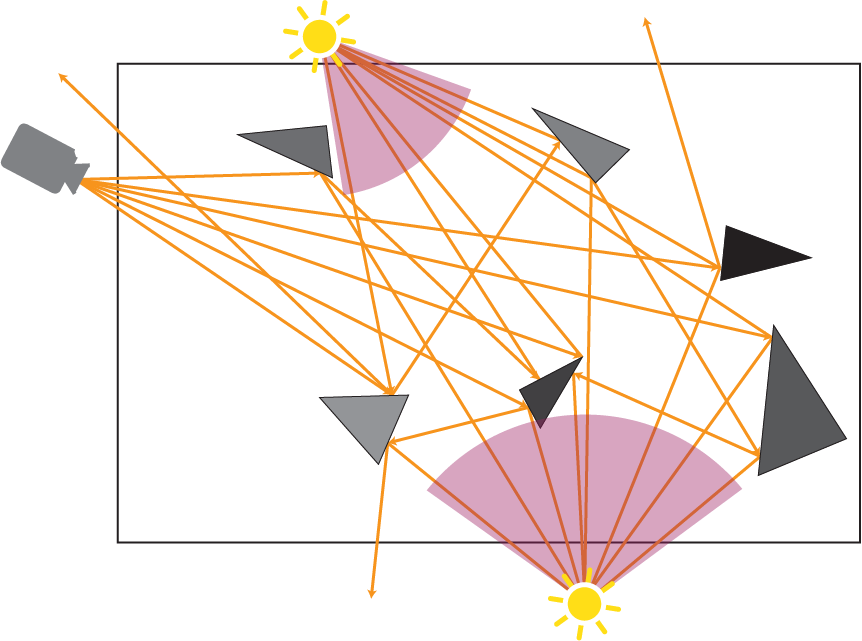
\includegraphics[width=\textwidth*\real{0.45}]{Images/with_importance_sampling.png}
	}
    \caption{With importance sampling rays are not distributed uniformly in the scene, but some artifacts naturally arise.}
    \label{fig:non_uniform_rays}
\end{figure}

Since rays are not distributed uniformly in the scene, it means that we cannot interpret the surface area of the AABB as related to the probability a ray hits it (figure \ref{fig:area_probability_visual}). For example, if an almost flat, but long AABB is present in a region where rays are parallel to the longest side of the AABB, the probability one of the ray hits it is very low. This wouldn't be reflected by the surface area of the AABB, which would assume a big value because of its long side. This can be visualized in the image below (\ref{fig:flat_long_aabb}).

\begin{figure}[H]
    \centering
    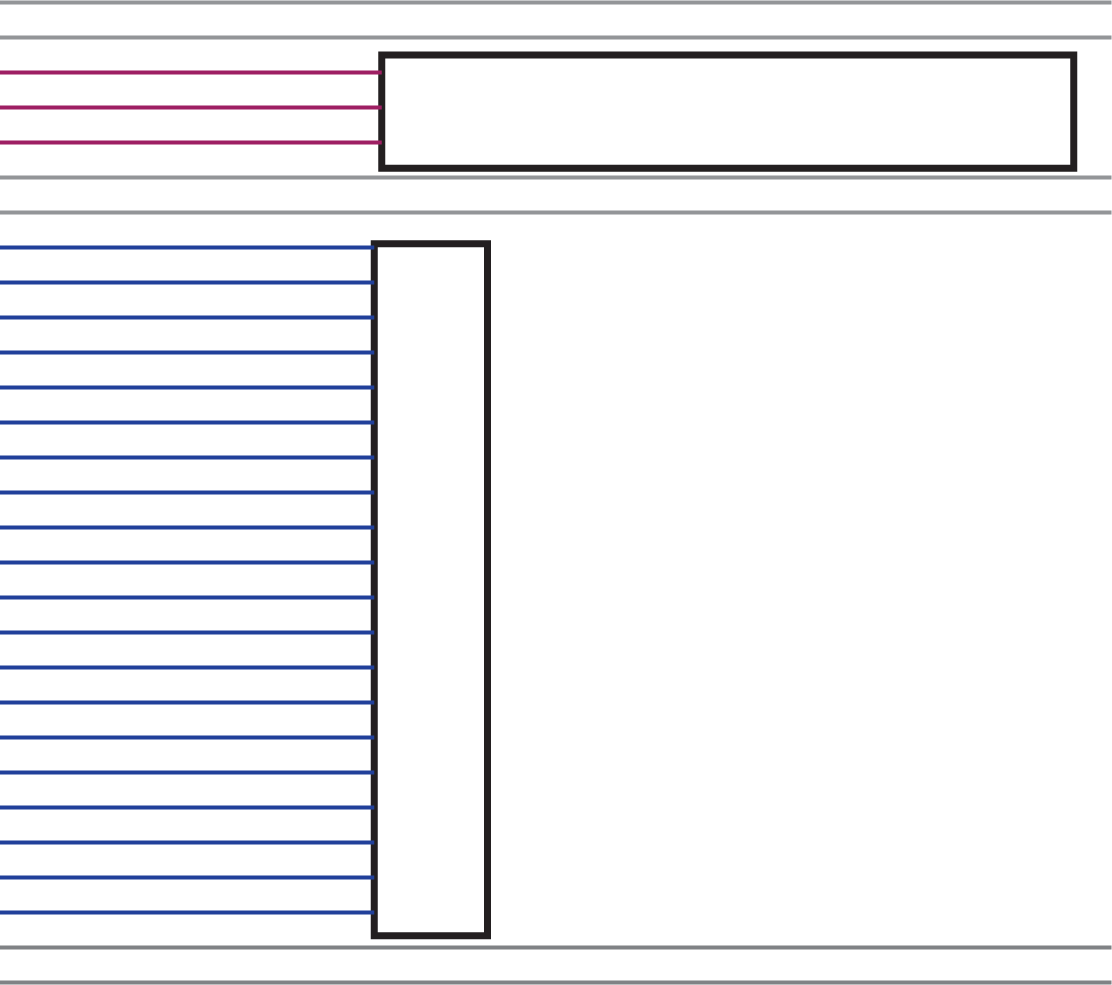
\includegraphics[width=\textwidth*\real{0.5}]{Images/rays_parallel_hit_prob.png}
    \caption{The two AABBs have the same hit probability according to SAH, but one of the two gets hit many more times in a region of parallel rays.}
    \label{fig:flat_long_aabb}
\end{figure}

The first novel contribution of this work is based exactly on this simple observation, and on the refutation of the last hypothesis of surface area heuristic. In the next sections we will describe two relevant ray distributions that organically form in the scenes, due to the use of direct light importance sampling.

In the past other works on this same topic have been written, but the proposed solution was based on a very different approach. For example, in this paper \cite{distribution_aware_bvhs} Yan Gu et al. proposed to modify an already existing BVH based on some statistics harvested during the previous frames. In summary, if a node is rarely hit, its subtree is collapsed, and all the triangles in the subtree are directly placed in the node, which becomes a leaf. Conversely, frequently hit leaves become internal nodes, and are further divided.

In our approach, instead, we try to directly build a BVH aware of the ray distribution. To achieve this we propose a new heuristic to calculate the probability that a node is hit by a ray: the Projected Area Heuristic (PAH).

\section{Parallel Ray Distribution} \label{sec:parallel_ray_distribution}
One of the relevant ray distributions that can naturally arise in a ray traced scene, where light importance sampling is used, is the distribution where rays are all parallel among themselves. This ray distribution usually arises in proximity of planar area light sources.

\begin{figure}[H]
    \centering
    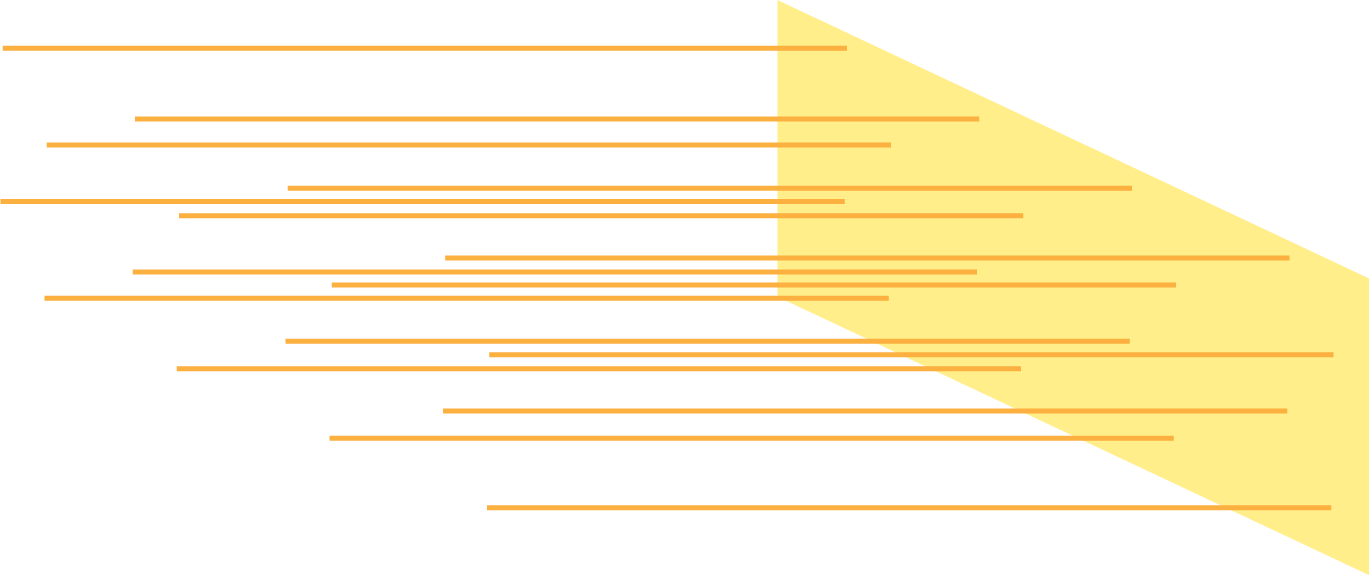
\includegraphics[width=\textwidth*\real{0.5}]{Images/plane_light_rays.png}
    \caption{Parallel rays distributions arise in proximity of planar area light sources.}
    \label{fig:parallel_rays_distribution}
\end{figure}

In a 3-dimensional region with such a ray distribution, we can estimate the probability an AABB is hit by a ray by computing the area projected by the AABB on the plane having a normal vector parallel to the rays.

Let us first analyze the case where the rays are parallel to one of the 3 cartesian axis, let's say $z$. In this case, the extension of an AABB in the $z$ direction is irrelevant, because it is impossible for a ray to hit the box on any face other than the $xy$ ones. Therefore, only the area of the $xy$ face is related to the probability that the AABB is hit.

We can generalize this idea to the case where the rays are parallel to an arbitrary direction by orthographically projecting the AABB on the plane normal to the rays. The area of the orthographic projection is directly related to the probability a ray hits the AABB.

\begin{figure}[H]
    \centering
    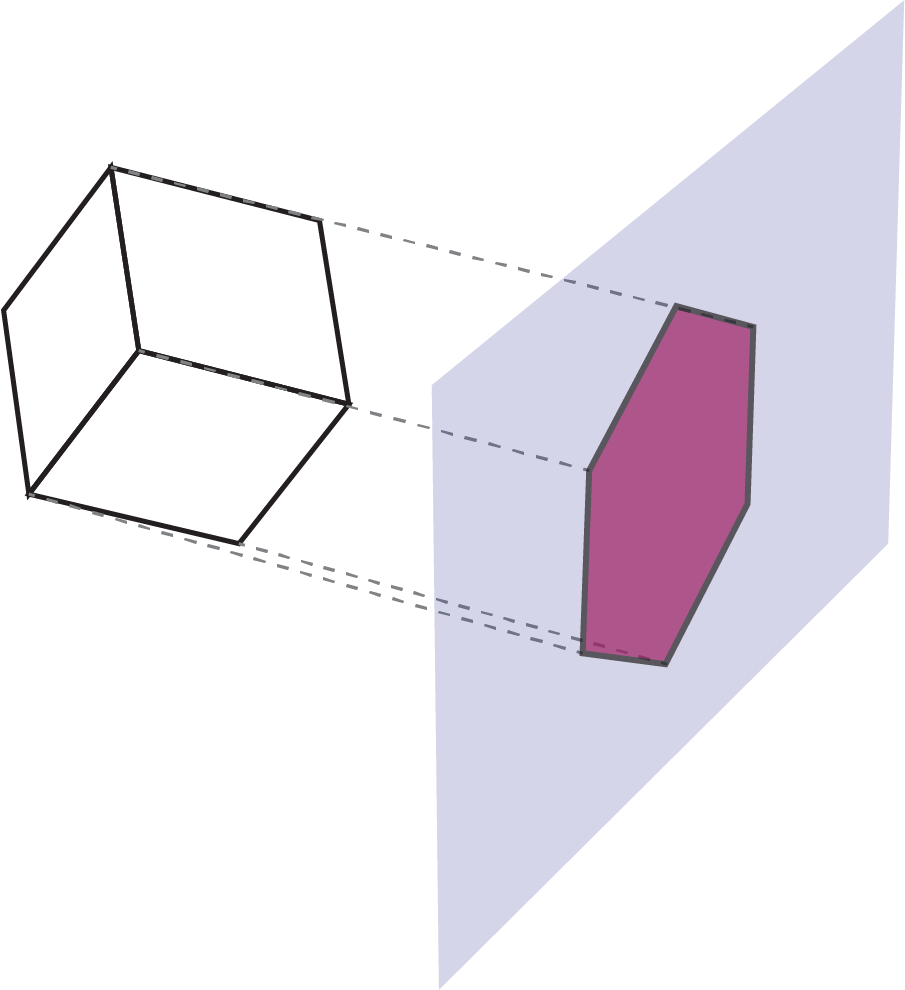
\includegraphics[width=\textwidth*\real{0.45}]{Images/ortho_projection.png}
    \caption{Orthographic projection of an AABB.}
    \label{fig:aabb_ortho_projection}
\end{figure}

The details of our implementation will be extensively discussed in section \ref{ch:implementation}.

\section{Point Ray Distribution} \label{sec:point_ray_distribution}
Another ray distribution commonly found in proximity of point lights is what we call the point ray distribution. In this distribution, rays all pass through the same point in 3D space, creating a radial pattern over a solid angle, as it is shown in the figure below.

\begin{figure}[H]
    \centering
    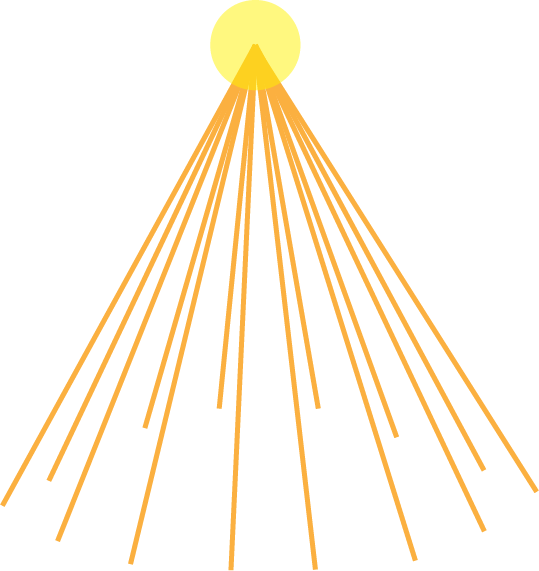
\includegraphics[width=\textwidth*\real{0.3}]{Images/point_light_rays.png}
    \caption{Point rays distributions arise in proximity of point light sources.}
    \label{fig:point_rays_distribution}
\end{figure}

Also in this case we can observe a relationship between the probability an AABB in this region is hit by a ray, and the area of the projection of said AABB. However, this time, the projection to estimate the hit probability is the perspective projection. The point all the rays in this region pass through can be interpreted as the focal point of the perspective. The projection plane can be placed at any distance from the focal point. Indeed, while it is true that by placing the plane at different positions we would get projections of different absolute sizes, it is also true that what we are really interested in is the relative area among the AABBs projected on the same plane. Indeed, as it is possible to see from the formula in section \ref{ssec:cost_computation} that we will report here:
$$p(ray\; hits\; K) = \frac{Area_K}{Area_{root}}$$
The hit probability $p$ is computed as the ratio between two areas.

\begin{figure}[H]
    \centering
    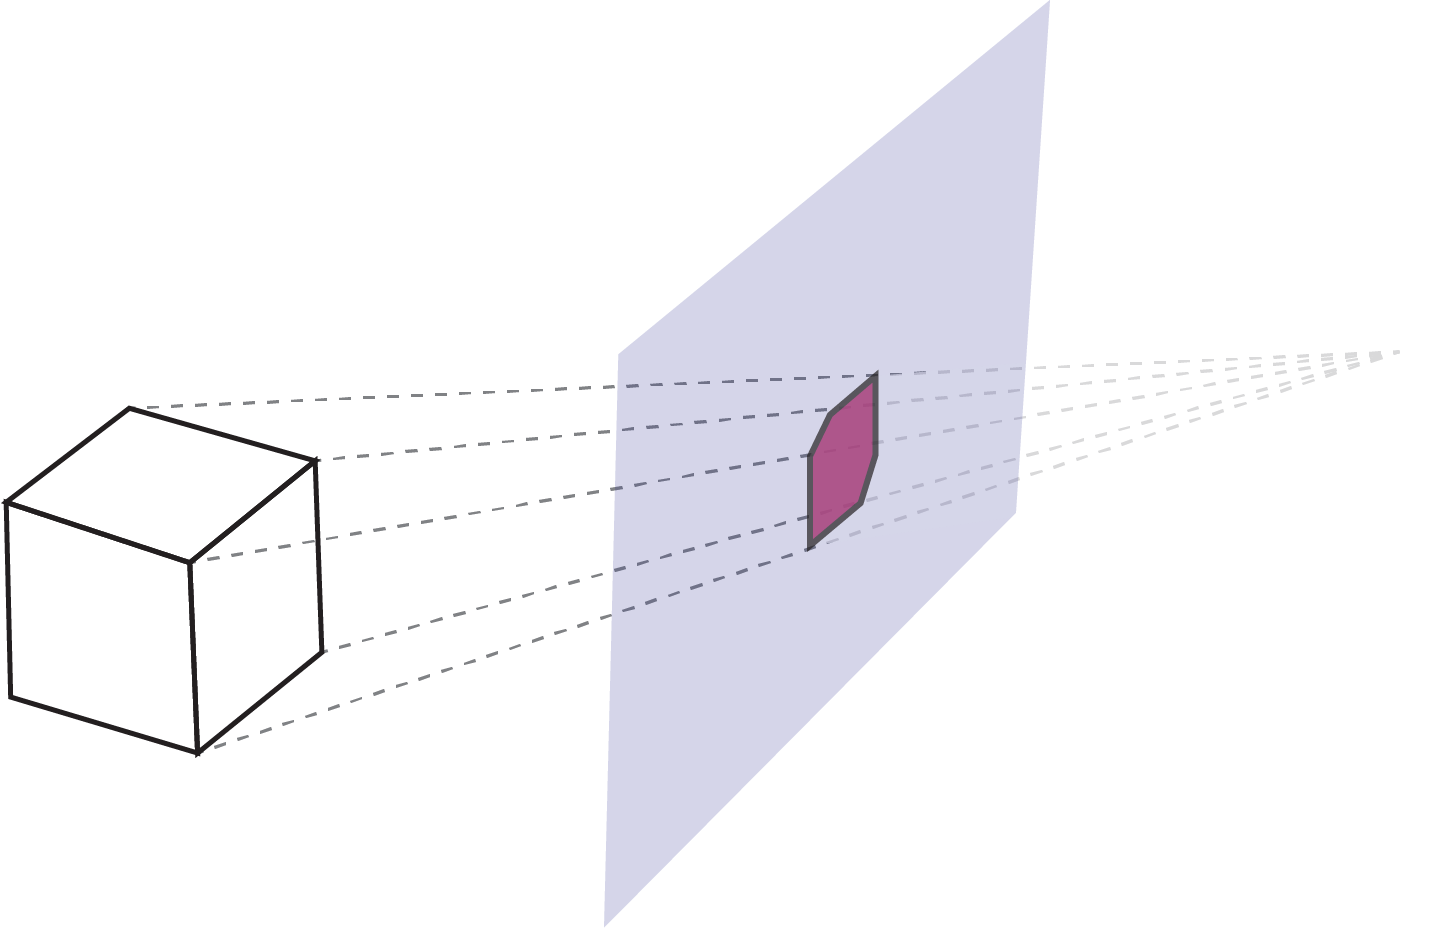
\includegraphics[width=\textwidth*\real{0.6}]{Images/perspective_projection.png}
    \caption{Perspective projection of an AABB.}
    \label{fig:aabb_perspective_projection}
\end{figure}

\section{The Projected Area Heuristic} \label{sec:projected_area_heuristic}
In the last two sections (\ref{sec:parallel_ray_distribution} and \ref{sec:point_ray_distribution}) we have seen how computing the projected area where there are certain ray distributions can be a better estimate for the probability that a ray hits an AABB, compared to the surface area. In simple words, this happens because some parts of the AABB are less likely (if at all) to be hit by a ray depending on their orientation, compared to the rays present in that 3D region. 

With this notion, it is now easy to define a heuristic to be used during BVH construction and another one for BVH evaluation. Indeed we can use the exact same formulae used for the surface area heuristic, but with the projected area in place of the surface area of the AABBs:
$$Cost_{PAH}(K) = \frac{ProjArea_K}{ProjArea_{root}} \cdot \#triangles_K \cdot 1.2$$
$$Cost_{PAH}(BVH) = \sum_{L \in leaf\; nodes} \frac{ProjArea_L}{ProjArea_{root}} \cdot \#triangles_L \cdot 1.2 + \sum_{I \in internal\; nodes} \frac{ProjArea_I}{ProjArea_{root}} \cdot 2 \cdot 1$$

With this heuristic it is possible to build a BVH for a portion of the scene where there is a certain ray distribution. If there is a parallel ray distribution, the orthographic projected area will be used. Instead, if there is a point ray distribution, perspective projection should be used.

However, in a scene, there likely is more than a single and global ray distribution. It is possible that ray distributions are localized in definite regions of the scene. This means that, rather than building a single and global BVH valid for all the scene, it is necessary to build partial and localized BVHs for specific regions. This is the main topic of the next chapter \ref{ch:multi_influence_areas}.

\begin{figure}[H]
    \centering
    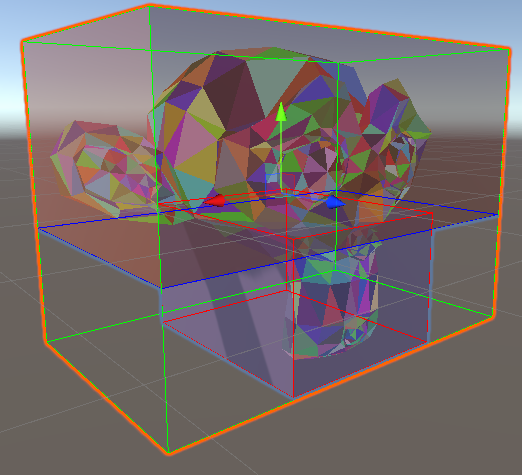
\includegraphics[width=\textwidth]{Images/suzanne_root_visualizer.png}
    \caption{A BVH seen in our Unity visualizer. The father node is green, and its two children are red and blue.}
    \label{fig:suzanne_root_visualizer}
\end{figure}

\chapter{Multiple Influence Areas and the Top Level Structure} \label{ch:multi_influence_areas}
In this chapter we will show how it is possible to deal with a scene where there are multiple localized ray distributions. We will first introduce the problem in detail and with visual examples, then we will define the concept of ray affinity to region where a relevant ray distribution is present. Eventually we will show how a scene with multiple ray distributions can be traversed by a ray. In this chapter we won't explain all the implementation details of the solution we propose, that will instead be discussed in section \ref{sec:top_level}.

As we have touched on in the last chapter, while ray tracing a scene, it is likely that more than a single relevant ray distribution appears. It is even more likely that, even if only one relevant distribution is present, it doesn't cover the entirety of the scene. For cases like these, it is necessary to be able to recognize whether a ray is affine to a certain ray distribution present in a scene. In case the ray is affine, we can use the BVH built with PAH on that part of the scene to find the first intersection. In case it is not affine, we must fall back to a global BVH, covering the whole scene. The definition of the term \textit{affine} is given in the next section (\ref{sec:ray_influence_area_affinity}).

\begin{figure}[]
    \centering
    
\includegraphics[width=\textwidth*\real{0.55}]{Images/multiple_influence_areas.png}
    \caption{A scene with multiple relevant ray distributions.}
    \label{fig:multiple_ray_distributions}
\end{figure}

From this point on, we will refer to a 3D region of a scene where a relevant ray distribution is present as influence area. If the ray distribution is parallel (section \ref{sec:parallel_ray_distribution}), we call the region \textit{plane influence area}. If the ray distribution is radial (section \ref{sec:point_ray_distribution}), the influence area is qualified as \textit{point influence area}. Each influence area has an associated BVH (also called local BVH) built with PAH, where the projection method (orthographic or perspective) is the corresponding one to the ray distribution of the influence area.

Influence areas must first be localized in the scene. To do so, we decided to encode a plane influence area as an oriented bounding box (section \ref{ssec:obb}). The rays start from one of the faces of the OBB, and are perpendicular to it. For what concerns point influence areas, the most natural bounding volume to localize them is 3D is a frustum (section \ref{ssec:frustum}). Rays start from the near plane of the frustum, and go toward the far plane. The direction of any of the ray can be obtained by connecting the origin of the ray on the near plane to the focal point of the frustum.

\begin{figure}[H]
    \centering
	\subfloat[Plane influence area]{
    	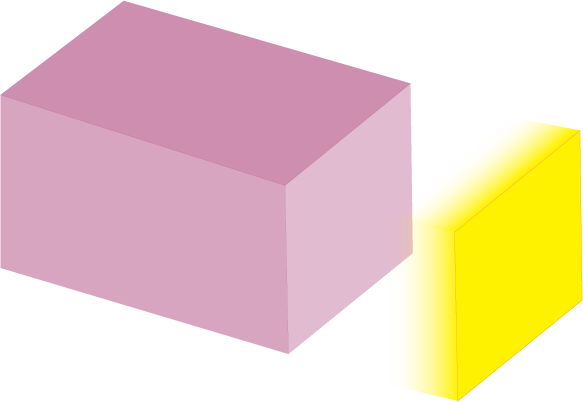
\includegraphics[width=\textwidth*\real{0.35}]{Images/obb_3d.png}
	}
	\qquad
	\subfloat[Point influence area]{
    	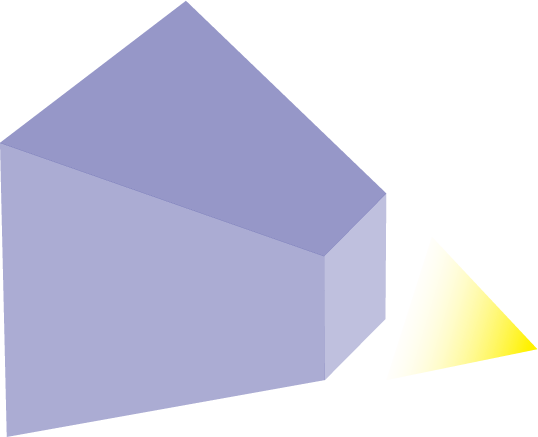
\includegraphics[width=\textwidth*\real{0.35}]{Images/frustum_3d.png}
	}
    \caption{Plane influence areas are described by OBBs, whereas point influence areas are described by frustums.}
    \label{fig:influence_areas}
\end{figure}

\section{Ray-Influence Area Affinity} \label{sec:ray_influence_area_affinity}
The first necessary condition to have a ray that is affine to an influence area, is that the origin of the ray is inside the influence area. To do so it is possible to use the algorithms described in appendices \ref{sec:point_inside_aabb} and \ref{sec:point_inside_frustum}, but can be made more efficient, as described in section \ref{sec:top_level_structure}.

The second necessary condition is that the direction of the ray fits with the direction of the rays in the influence area. This is extremely simple to verify for plane influence areas, where all the rays must have the same direction. Verifying this second condition for point influence areas is more complex, but can be achieved by connecting the origin of the ray with the focal point, and checking that the direction of this vector is parallel with the direction of the ray, as it is possible to visualize in figure \ref{fig:affine_direction}.

It is possible to introduce a tolerance in the verification of the second condition. The bigger the tolerance, the more rays will be affine, but if the tolerance gets too large also rays that don't benefit from the BVH built with PAH will traverse it.

If a ray is affine to an influence area, it can use the BVH associated with the influence area during traversal.

\begin{figure}[]
    \centering
    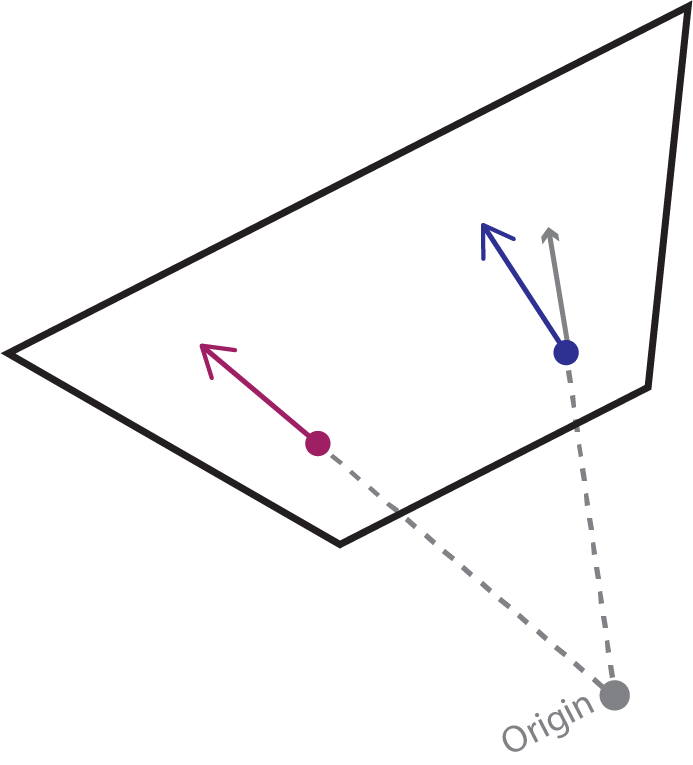
\includegraphics[width=\textwidth*\real{0.35}]{Images/direction_affinity.png}
    \caption{Visualization of the method to verify if the direction of a ray is affine with a point influence area.}
    \label{fig:affine_direction}
\end{figure}

\section{Local and Global BVHs} \label{sec:local_and_global_bvhs}

Since influence areas are localized in specific regions of the scene, it would be wasteful to build the associated PAH BVH on all the geometry present. The associated BVH is therefore built by considering only the triangles inside the influence area. It is important to note that a triangle is considered inside the influence area if at least one of its vertices or edges is inside. This conservative definition of the \textit{inside} concept is necessary to avoid errors in the traversal. Indeed, if we used a less restrictive definition, such as by considering the barycenter, it would be possible to find the wrong closest hit while tracing a ray, as it is possible to observe in figure \ref{fig:conservative_inside}.

\begin{figure}[H]
    \centering
    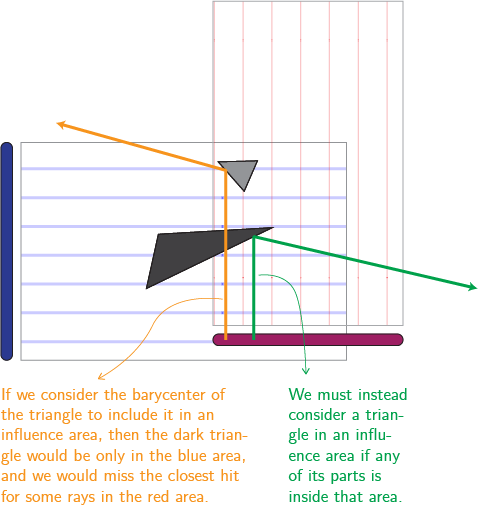
\includegraphics[width=\textwidth*\real{0.55}]{Images/double_area.png}
    \caption{Example of why it is necessary to use a conservative approach.}
    \label{fig:conservative_inside}
\end{figure}

Influence areas do not guarantee to cover the whole scene. It is indeed more frequent that regions of the scene don't have any particular ray distribution. In this case, those triangles that are not inside any influence area, would not be part of any BVH, and would therefore be invisible to rays during traversal. For this very reason, it is necessary to build a global BVH for the whole scene. In our implementation, this BVH is built by using surface area heuristic.

When a ray traverses a local BVH and no hit is found, it is necessary to traverse the global BVH. It is indeed possible to find a hit with triangles that are not inside the influence area of the local BVH, as it can be observed in figure \ref{fig:outside_area}. However, if a ray is found in the local BVH, it is guaranteed for it to be the closest one, as shown in figure \ref{fig:conservative_inside}.

\begin{figure}[H]
    \centering
    \includegraphics[width=\textwidth*\real{0.55}]{Images/outside_area.png}
    \caption{Example of how it is possible that a hit is found in the global BVH, but not in the local one.}
    \label{fig:outside_area}
\end{figure}

\section{Top Level Structure} \label{sec:top_level_structure}
At the beginning of this chapter, we stated that the first affinity criterion between a ray and an influence area is that the origin of the ray is inside the influence area. We have also seen how BVHs associated with influence areas contain only triangles that are inside the influence area. It is therefore of paramount importance to have a fast method to detect whether a point is inside a certain 3D region of the scene. 

In our implementation we tried to tackle this problem by using two different approaches. We will now briefly describe them from a theoretical point of view. All the details of our implementation can be found in section \ref{sec:top_level}.

The first approach is to use algorithms described in appendices \ref{sec:point_inside_aabb} and \ref{sec:point_inside_frustum}, and each time we want to check if a point is inside any influence area, iterate over all the influence areas present in the scene. The complexity of this method linearly depends on the amount of influence areas present in the scene. Moreover, the algorithms to find out if a point is inside an OBB or a frustum are not cheap, especially in a scenario where they must be used for every single ray. On the other hand, all the influence areas can be easily stored in an array, therefore there is no overhead in building an ad-hoc structure.

On the opposite side of the spectrum there is the second method we propose. In this case we build an octree, where each leaf contains the influence areas that overlap with it. Building such an octree is not trivial, and it is diffusely described in section \ref{ssec:top_level_octree}. However, once the octree is built, it is extremely cheap to find out what are the influence areas containing any given 3D point. It is indeed sufficient to traverse the octree and read the data in the leaf. Considering that it is not necessary to have extremely fine-grained octrees to achieve good results with PAH, we consider octrees the better choice as top level structure. More on the performance can be found in chapter \ref{ch:experimental_results}.

\begin{figure}[H]
    \centering
    \includegraphics[width=\textwidth]{Images/octree_dense_wireframe.png}
    \caption{The wireframe of the octree built on a single point influence area.}
    \label{fig:octree_dense_wireframe}
\end{figure}

\chapter{Splitting Plane Facing Heuristic} \label{ch:splitting_plane_facing_heuristic}
In chapter \ref{ch:projected_area_heuristic} we described the first heuristic we propose in this thesis. With PAH it is possible to estimate better the probability a ray hits AABBs in a region of the scene where relevant ray distributions are present. This enables us to have more accurate information on how to split a node at each level, during BVH construction. However, as we stated in section \ref{ssec:triangles_splitting}, another important step in building high-quality BVHs is the choosing of the orientation of the splitting plane. In this chapter we will propose a novel method to select the splitting plane, whose main aim is to reduce the overlapping of the projected area of the children nodes. Its name is Splitting Plane Facing Heuristic (SPFH).

As extensively discussed in section \ref{ssec:triangles_splitting}, in today's BVH builders, during the triangles splitting phase, usually only one plane orientation is selected. With this strategy it is possible to trade build time for accuracy. Indeed, fewer splitting planes must be attempted at each step, but, at the same time, it is possible to miss some relevant splits. Moreover, since the majority of BVHs use AABBs, the possible splitting plane orientations among which to choose one are only 3, parallel to each cartesian axis.

Before continuing to the next paragraph, it is important to talk about the language we will use. In particular, the expression \textit{cut along the $K$ axis} means that the plane we are using to split the AABB into two children has a normal that is parallel to the specified axis $K$. Furthermore, we use the expression \textit{$K$ axis plane} to denote a plane whose normal is parallel to the $K$ cartesian axis.

The most used heuristic to choose the splitting plane orientation, is to cut along the longest dimension of the AABB. The main idea behind this method is that, the longer the axis of the AABB, the more chances there are to cut off space effectively.

Our idea instead, based on \cite{bvh_overlapping_metric}, is to use the information about the ray directions in a specific region of the scene, in order to divide a node such that it is less likely that its two children can be hit by the same ray. We can quantify the likeliness that two AABBs are hit by the same ray, by computing the projection of the overlapped area between the two. The projection, as we described in chapter \ref{ch:projected_area_heuristic}, is an orthographic projection in case of a plane influence area, and a perspective projection in case of a point influence area.

\begin{figure}[H]
    \centering
    \includegraphics[width=\textwidth*\real{0.6}]{Images/projection_overlapping.png}
    \caption{Overlapping projected area between two nodes' AABBs.}
    \label{fig:overlapping_projected_area}
\end{figure}

It is possible to compute the overlapping area between two AABBs projections with the algorithm described in appendix \ref{sec:2dHull_culling}. However, doing so for each possible triangles split at each BVH level would be too expensive from a computational point of view.

We therefore decided to use a heuristic to find out which is the best cartesian axis to cut along, so that it is most likely to have splits with not much overlapping. We found out that, the more the ray direction of the influence area is perpendicular to the normal of the splitting plane, the less likely it is for the two children's AABBs to have a large overlapping area.

We can first analyze the simplest case (figure \ref{fig:ray_facing_simplest_case}), where there is a plane influence area with rays direction parallel to the $z$ axis. In this case, the ray direction is perpendicular to the $x$ and $y$ cartesian axes, which define two possible splitting plane orientations. Instead, it is parallel to the $z$ cartesian axis, which defines the last possible plane orientation (considering we use the optimization where only the 3 cartesian planes are used). If we consider a uniform distribution of the triangles in the father node, it is clear that, if we divide its AABB with the $z$ axis plane, it is extremely likely for a single ray to hit both of the children. At the same time, it is almost impossible for a ray to hit both children if we use the other two planes to split the father node's AABB. Indeed, in this last case, the only possible source of overlapping is given by the fact that triangles are not point-like entities, but have an extension; therefore it is possible that the splitting plane, which partitions the triangles based on their barycenter, splits the vertices of a triangle in both the half-spaces generated by the plane, as we discussed in section \ref{ssec:triangles_splitting} and as it is possible to observe in figure \ref{fig:triangle_splitting_extension}.

\begin{figure}[H]
	\centering
	\includegraphics[width=\textwidth*\real{0.45}]{Images/overlapping_by_extension.png}
	\caption{Overlapping caused by the triangle extension.}
	\label{fig:triangle_splitting_extension}
\end{figure}

\begin{figure}[H]
    \centering
	\subfloat[$x$ axis plane]{
    	\includegraphics[scale=0.125]{Images/x_axis_plane.png}
	}
	\qquad
	\subfloat[$y$ axis plane]{
    	\includegraphics[scale=0.125]{Images/y_axis_plane.png}
	}
	\qquad
	\subfloat[$z$ axis plane]{
    	\includegraphics[scale=0.125]{Images/z_axis_plane.png}
	}
    \caption{Visual illustration of the possible splitting plane orientations and how a ray can hit the children AABBs.}
    \label{fig:ray_facing_simplest_case}
\end{figure}

The same reasoning can be carried out with influence areas with arbitrary rays direction. However, it is important to understand that, if there isn't a clear cartesian axis the rays are perpendicular to, using SPFH to choose the splitting plane direction becomes useless. Let's imagine a case in 2 dimensions where the rays have an angle of 45°. In this case, if we adapt the reasoning in the last paragraph to the 2D scenario, we can see that choosing to cut along the $x$ or $y$ axes makes no difference. In such a case it is better to fall back to a known heuristic, such as the longest axis one.

For this reason, in our implementation, we decided to assign a quality value to each one of the three possible orientations of the splitting plane. We then use it to decide which is the best orientation to choose, or, in case none is good enough, to fall back to the longest axis heuristic.

The function to compute the quality value for the three cartesian axes takes into account how much the influence area's rays direction is parallel to each one of them. Given that the ray direction is named $v$:
\begin{align*}
	quality\;of\;x\;axis &= \frac{|v_x|}{|v_x|+|v_y|+|v_z|} \\
	quality\;of\;y\;axis &= \frac{|v_y|}{|v_x|+|v_y|+|v_z|} \\
	quality\;of\;z\;axis &= \frac{|v_z|}{|v_x|+|v_y|+|v_z|}
\end{align*}

In other words, we compute how much each cartesian axis direction is parallel to the rays direction, in percentage. In this way we can clearly quantify how much rays are parallel to each cartesian axis. At this point, it is possible to set a threshold over which a cartesian axis is deemed \textit{too much parallel} to the direction of the rays to be a good choice for the splitting plane. If all the cartesian axes are over the threshold, we can fall back to the longest axis heuristic.

It is also possible that two cartesian axes have a very low quality value. In the example of the simplest case scenario, that can be found a few paragraphs above, the quality values are $0\%$ for the $x$ and $y$ axes and $100\%$ for the $z$ axis. In this case, since both $x$ and $y$ are good candidates for the splitting plane, one is chosen arbitrarily. After a split is found, if the cost of the two children nodes is above a certain threshold, then also the second axis is tried. The threshold can be dynamically adjusted based on the quality of the axes in contention. For example, if instead of a quality value of $0\%$, as in the example above, the two axes had a quality value of $10\%$, then the threshold could be adjusted to a higher value, because it is less likely to find a good split with a quality value of $10\%$ rather than $0\%$.

The same concept can be applied to the use of the fallback method. Before we stated that the fallback method is used when the quality values of all the axes are above a certain static threshold. However, it is also possible to set our implementation so that the fallback method is also used when, after a split, the two children nodes have a cost over a customizable fallback threshold.

A more in-depth explanation of our algorithm can be found in section \ref{ssec:splitting_plane_implementation}.

Thanks to the customizable thresholds it is possible to make our algorithm more or less accurate in the choosing of the splitting plane. Having a more accurate algorithm can yield higher-quality BVHs, at the cost of a higher construction time.

Another important factor in the effectiveness of SPFH is the type of influence area. Until now we talked about \textit{the rays direction of the influence area}. If this definition can be unequivocably given to plane influence areas, where all the rays face the same direction (chapter \ref{ch:multi_influence_areas}), the same cannot be stated for point influence areas, where the rays face many different directions. In the case of point influence area, the central direction can be considered as the direction of all the rays. However, if the point influence area have a large spread in its rays' directions, then this approximation doesn't hold. In such cases, it is not possible to use SPFH effectively, and it is therefore advised to fall back to the longest area heuristic.
	
The discussion about the quality of the BVHs built with the splitting plane facing heuristic (SPFH) can be found in chapter \ref{ch:experimental_results}.

\chapter{Implementation} \label{ch:implementation}
In this chapter we will analyze how we built the framework that allowed us to test the novel techniques we explained in previous chapters, and to compare the results with other methods.
We will explain all the implementation details we skipped in previous chapters, however we won't dwell on the performance, which is the main subject of chapter \ref{ch:experimental_results}.

At the beginning of the development we used to write prototypes in C\#, in order to be able to immediately visualize the results in Unity. However, as we were convinced of the validity of our ideas, we decided to write code in C++, in order to have more control over it and be independent from a specific engine for visualization purposes. The code of our project can be found on this GitHub repository: \url{TODO}.

Furthermore, it is possible to read the documentation of our code, generated with Doxygen\footnote{\url{https://www.doxygen.nl/}}, at this address: \url{TODO}. We decided to provide the documentation in order to help future developments. As explained in the next chapters, we tried to make the framework generic and flexible, in order to be able to test different algorithms without completely rewriting the system.

In parallel with the development of the framework to test our algorithms, we also developed an independent visualizer in Unity. The visualizer receives a JSON generated by the C++ framework, and shows the generated data structures over a scene (usually the BVHs). We decided to build the Unity visualizer in order to help us graphically visualize the results of our algorithms. This approach proved very useful to fix bugs and identify pitfalls in our approaches. We won't describe the Unity visualizer in this thesis, but the code can be found at this address: \url{TODO}.

Despite the framework being written in C++, in the next sections we will present the algorithms in a language-agnostic way: our focus is on the concepts rather than the idiosyncrasies of a specific language.

\section{BVH} \label{sec:bvh}
In this section, we will present the concepts about the class that in our implementation is responsible for representing, building and traversing a BVH.

The main data members of our $Bvh$ class are the following:
\begin{algorithm}[H]
	\begin{algorithmic}
		\Class{$Bvh$}
		\Member{$root$}{$Node$}
		\Member{$influenceArea$}{$InfluenceArea*$}
		\Member{$computeCost$}{$function*$}
		\Member{$chooseSplittingPlanes$}{$function*$}
		\Member{$shouldStop$}{$function*$}
		\Member{$properties$}{$Properties[]$}
	\end{algorithmic}
\end{algorithm} 

We store the influence area the BVH is associated to. The pointer can be left $null$ in case the BVH is not associated with any influence area, such as for the scene-global BVH.

The three functions are customizable, and are customization point for the BVH construction, as explained in the algorithm in section \ref{ssec:bvh_construction}.

We also store the root node of the BVH. Each node is a member of the $Node$ class, whose main members are:
\begin{algorithm}[H]
	\begin{algorithmic}
		\Class{$Node$}
		\Member{$aabb$}{$Aabb$}
		\Member{$leftChild$}{$Node*$}
		\Member{$rightChild$}{$Node*$}
		\Member{$triangles$}{$Triangle$}
	\end{algorithmic}
\end{algorithm} 

Since a BVH is a complete tree, a leaf node can be detected by the absence of its children.

An important note is that, in our framework, we are also interested in getting information about the timing and performance of the BVH builder. For this purpose it is possible to add time information to a $Node$, collected during construction, by enabling a C++ macro. The information in each node can later be analyzed, as it is explained in section \ref{sec:bvh_analyzer}.

The $properies$ are values upon which depends how the BVH is built. We will now list and explain some of them:
\begin{description} 
	\item[\boldmath$maxLeafCost$] If a node has a cost (PAH or SAH depending on the cost strategy used) less than this threshold, it is a leaf.
	\item[\boldmath$maxLeafArea$] If a node has an area (projected or surface depending on the cost strategy used) less than this threshold, it is a leaf.
	\item[\boldmath$maxLeafHitProbability$] If the hit probability (section \ref{ssec:cost_computation}) of this node is less than this threshold, it is a leaf.
	\item[\boldmath$maxTrianglesPerLeaf$] If a node has fewer triangles than this threshold, it is a leaf.
	\item[\boldmath$maxLevels$] If a node is at a level higher than this threshold, it is a leaf.
	\item[\boldmath$bins$] How many cuts to try to split a node into its children. A higher value generates more accurate BVHs, but is is also more expensive (section \ref{ssec:triangles_splitting}).
	\item[\boldmath$maxNonFallbackLevels$] If a node is at a level higher than this threshold, the specified fallback strategies (usually SAH and longest splitting plane heuristic) will be used to split it into children. This can be used to avoid using an expensive strategy (such as PAH) even at deep levels, where there is less to gain.
	\item[\boldmath$splitPlaneQualityThreshold$] $[0, 1]$. If the quality of the split plane (chapter \ref{ch:splitting_plane_facing_heuristic}) is less than this threshold, two things can happen: if a satisfactory split plane has already been found (look at the next two properties), it is used; if not, use the fallback strategy to find the splitting plane. A low value will leave the algorithm find the best splitting plane more times, but will slow the construction down. More details in section \ref{ssec:splitting_plane_implementation}.
	\item[\boldmath$acceptableChildrenFatherHitProbabilityRatio$] Defined as $\frac{leftChildHit\% + rightChildHit\%}{fatherHit\%}$. This value is used to determine if a splitting plane cut is acceptable when no more planes with the minimum quality are present. The value is used to approximate the overlapping of the two children nodes: in the ideal case (no overlapping) this value is less than 1. A low value forces the algorithm to use the fallback strategy more often, therefore will also slow the construction down. More details in section \ref{ssec:splitting_plane_implementation}.
	\item[\boldmath$excellentChildrenFatherHitProbabilityRatio$] Same as above, but in this case this value is compared with the best children found after each splitting plane cut: if such value is lower than this threshold, no more splitting planes are attempted, even if they had the required quality. This allows an early out during the search for the splitting plane. More details in section \ref{ssec:splitting_plane_implementation}.
\end{description}
	
A $Bvh$ can be built with the member $build$ function, which takes an array of $Triangles$ representing the scene as argument. The function has already been described in section \ref{ssec:bvh_construction}. Here we limit ourselves to remember that the function builds the BVH recursively, and uses the three customization functions cited above to decide how to build the BVH.

To traverse a $Bvh$ it is possible to use the $traverse$ function, which takes a $Ray$ as argument. The process will be detailed in section \ref{ssec:traversal}.


\subsection{Splitting Plane Search Implementation} \label{ssec:splitting_plane_implementation}
In this section we will analyze in more detail how the selection of the best splitting plane for each node is implemented.

The function $chooseSplittingPlanes$ is required to return a list of cartesian axes, associated with their quality value. This function always returns all the three axes, even if the quality of some of them is extremely low. More info about this topic can be found in chapter \ref{ch:splitting_plane_facing_heuristic}.

In the $build$ function of the $Bvh$, we iterate over the axes returned by the $chooseSplittingPlanes$ function, and, for each one of them, we use the binned approach to look for a good way of splitting the node into two children. However, some of the properties listed above, can influence what axes returned by $chooseSplittingPlanes$ are actually used:

\begin{algorithm}[H]
	\caption{How the $build$ function chooses what axes to use to look for the best split.}
	\begin{algorithmic}[1]
		\State{$...$}
		\Let{$axes$}{$chooseSplittingPlanes(...)$}
		\ForAll{$\langle axis, quality \rangle \in axes$}
			\Let{$bestCutSoFarQuality$}{$\frac{bestLeftCostSoFar.hitProbability + bestRightCostSoFar.hitProbability}{fatherHitProbability}$}
			\If{$bestCutSoFarQuality \leq excellentChildrenFatherHitProbabilityRatio$}
				\State{$\textbf{break}$}
				\EndIf
				\Let{$forceFallback$}{$false$}
				\If{$quality < splitPlaneQualityThreshold$}
					\If{$bestCutSoFarQuality \leq acceptableChildrenFatherHitProbRatio$}
						\State{$\textbf{break}$}
					\EndIf
				\EndIf
				\Let{$forceFallback$}{$true$}
				\Let{$axis$}{$chooseSplittingPlanes(forceFallback, ...)[0]$}
			\State{$...$}\Comment{start of the binned search phase with $axis$ as splitting plane normal...}
		\EndFor
	\end{algorithmic}
\end{algorithm} 

In simple words, if an axis is \textit{excellent}, meaning that a very good triangle split has been found by using it, no more cuts are attempted, no matter what (line 5).

Instead, if no more axes are good enough (based on the threshold at line 8), then, if a cut has already been found in previous steps and its quality is \textit{acceptable} (line 9), it is used as splitting plane. Otherwise the fallback method (always SAH in our test cases) is used to find a splitting plane (line 11 and 12).

It is recommended that the $build$ function often looks for the best split by using just one plane, as we suggested in section \ref{ssec:triangles_splitting}. It is possible to achieve this by choosing a not-too-high threshold for what is considered an \textit{acceptable} cut, or by rising the $splitPlaneQualityThreshold$ to discern a good splitting plane from a bad one. Using more than one splitting plane should happen only in exceptional cases if this algorithm is to be used in a real-time scenario.

\subsection{Traversal} \label{ssec:traversal}
The BVH traversal process is more straightforward than the build process. The main data structure used to traverse the BVH is the queue:

\begin{algorithm}[H]
	\caption{How the $build$ function chooses what axes to use to look for the best split.}
	\begin{algorithmic}[1]
		\Function{traverse}{$ray$}
		\Let{$closestHitTriangle$}{$null$}
		\Let{$closestHitDist$}{$\infty$}
		\Let{$toVisit$}{$queue$}
		\State{$toVisit.push(root)$}
		\While{$\ANot toVisit.empty()$}
			\Let{$current$}{$toVisit.pop()$}
			\Let{$hitInfo$}{$collision(ray, current)$}
			\If{$hitInfo \neq null \AAnd hitInfo.distance < closestHit$}
				\If{$current.isLeaf()$}
					\ForAll{$triangle \in current.triangles$}
						\Let{$triangleHitInfo$}{$collision(ray, triangle)$} \Comment{abbreviated to $thi$}
						\If{$thi \neq null \AAnd thi.distance < closestHit$}
							\Let{$closestHitTriangle$}{$triangle$}
							\Let{$closestHitDist$}{$thi.distance$}
						\EndIf
					\EndFor
				\Else
					\State{$toVisit.push(current.leftChild$)}
					\State{$toVisit.push(current.rightChild$)}
				\EndIf
			\EndIf
		\EndWhile
		\State \Return{$\langle closestHitTriangle, closestHitDist \rangle$}
		\EndFunction
	\end{algorithmic}
\end{algorithm} 

In our implementation we are interested in analyzing whether the BVH cost is accurate. For this reason we made some addition to the presented algorithm to artificially compute the real cost of the traversal of a BVH. In particular, we introduce a variable to keep track of the cost of the traversal which simulates the SAH or PAH. When we enter a leaf node, the value is incremented by $current.triangles.size() \cdot 1$. When a non leaf node is hit the value is incremented by $2 \cdot 1.2$. It is possible to observe the similarities with what we discussed in section \ref{ssec:cost_computation}.

\begin{figure}[H]
    \centering
    \includegraphics[width=\textwidth]{Images/suzanne_visualizer.png}
    \caption{The BVH built over the Blender Suzanne mesh, as seen in our visualizer.}
    \label{fig:suzanne_visualizer}
\end{figure}

\section{BVH Analyzer} \label{sec:bvh_analyzer}
In this section we will describe the class used to analyze a BVH and produce a JSON output, that can be passed to the Unity visualizer or to other analyzing tools.

One of the core points in our implementation of the BVH builder was to avoid as much as possible introducing overhead caused by procedures collecting data about the BVH. Nonetheless collecting information about the BVH was one of the most relevant interests of our research. To let these two necessities coexist, we decided to write a class that receives a BVH as input, along with some functions to analyze it, fully traverses it breadth-first, and outputs a JSON representing the BVH and the required information.

The most challenging part has been to let the user of the framework write its own data-collecting functions, and make it so that it was possible to collect virtually any statistic about the BVH by using these functions. At the end of the day we adopted an approach where the user must specify two functions for each category of data he or she wants to collect:
\begin{description}
	\item[Per-node functions] These functions are executed at each node during the traversal. They take as input the node itself and an object of a data type chosen by the user. This object is stored as a data member of the $BvhAnalyzer$ class\footnote{To achieve this in practice we store a C++ tuple as data member of the $BvhAnalyzer$. At compile time, by leveraging template metaprogramming, the user can specify what data types he or she wants to store inside this tuple.}, therefore it is persistent across the invocations on different nodes.
	\item[Final actions] These functions are executed at the end of the traversal of the BVH, and take as input the same object the corresponding per-node function uses. In this way, the per-node functions can store data on a \textit{BVH-global} variable, and this data can be processed at the end of the traversal.  
\end{description}

An example of per-node/final action pair is to calculate the PAH or SAH cost of a BVH: each per-node function computes the PAH or SAH cost for the node, appends it to the JSON of the current node, and adds its value to a global total cost. The final action reads the global total cost and outputs it to the JSON.

The same logic can be used, for example, to count the number of triangles (per-node and total), compute the siblings overlapping area (per-node and average, see chapter \ref{ch:splitting_plane_facing_heuristic}), save information about performance or simply count nodes.

\section{Regions} \label{sec:regions}
In this section we will analyze some of the data structures we used to describe regions of 3D space. These structures are then used in many parts of the codebase, such as in the BVH, as influence areas or in the top level structure. 

All the presented structures derive from the base $Region$ structure. This allows us to be able to interchange them easily. The $Region$ structure contains the following methods to be overridden:
\begin{description}
	\item[\boldmath$contains(point)$] Returns whether a point is inside the region. Used for AABBs for Regions top level structure (section \ref{ssec:top_level_aabbs}), and for octree top level structure construction and traversal (section \ref{ssec:top_level_octree}).
	\item[\boldmath$enclosingAabb()$] Returns the tightest AABB enclosing the region. Often used in pair with $contains(point)$ as rejection test (look at section \ref{ssec:aabb_for_obb}).
	\item[\boldmath$isCollidingWith(aabb)$] Returns whether the region is intersecting the specified AABB. Used in top level octree construction (section \ref{ssec:top_level_octree}).
	\item[\boldmath$fullyContains(aabb)$] Returns whether the region is fully enclosing the specified AABB. Used in top level octree construction (section \ref{ssec:top_level_octree}).
\end{description}

\subsection{Oriented Bounding Box} \label{ssec:obb}
An oriented bounding box is a region of 3D space enclosed in a rectangle parallelepiped. As mentioned in section \ref{ssec:the_bounding_volume_hierarchy}, OBBs can be used as bounding volume in a BVH. While providing a good approximation of the volume occupied by the primitives in many situations, they are quite expensive to intersect with a ray, therefore are not often employed as bounding boxes in state-of-the-art BVH builders. In our implementation we use them to describe a plane influence area, as shown in section \ref{ssec:plane_influence_area}.

In our implementation we describe a bounding box in this way:
\begin{algorithm}[H]
	\begin{algorithmic}
		\Class{$Obb$}
		\Member{$center$}{$Vector3$}
		\Member{$forward$}{$Vector3*$}
		\Member{$right$}{$Vector3*$}
		\Member{$up$}{$Vector3$}
		\Member{$halfSize$}{$Vector3$}
	\end{algorithmic}
\end{algorithm} 

We decided to store all the three main axes of the OBB because they are used in the SAT algorithm, as described in section \ref{sec:frustum_aabb_intersection}, and also in the algorithm to detect if a point is inside the OBB.

The $halfSize$ member stores the extents of the OBB starting from the center and toward the 3 main directions.

\subsubsection*{$contains(point)$}
In order to detect if a point is inside an OBB, we project its distance vector from the center, via a dot product, to all the three main axes: if all three projections are shorter than the half size in the corresponding direction, the point is inside.

\begin{figure}[H]
    \centering
    \includegraphics[width=\textwidth*\real{0.5}]{Images/point_obb_test.png}
    \caption{Check to detect if a point is inside an OBB.}
    \label{fig:oobb_contains}
\end{figure}

\subsubsection*{$enclosingAabb()$}
To compute the tightest enclosing AABB, we iterate over all the 8 vertices of the OBB and compute the maximum and minimum in every dimension.

\subsubsection*{$isCollidingWith(aabb)$}
We use a simplified version the separanting axis test (section \ref{sec:frustum_aabb_intersection}).

\subsubsection*{$fullyContains(aabb)$}
To check if an AABB is fully contained in the OBB, we simply check that all the vertices of the AABB are inside the OBB, by using the $contains(point)$ method.

\subsection{Axis Aligned Bounding Box} \label{ssec:aabb}
An axis-aligned bounding box (AABB) is an OBB where the three main directions are constrained to be parallel to the three cartesian axes of the reference system. AABBs are the most used 3D region in our implementation. They are the key element of a BVH (section \ref{sec:bvh}), and are also used in the octree top level structure (section \ref{ssec:top_level_octree}).

The fact that AABB are, indeed, axis aligned, make them worse than OBBs as bounding volumes, however make them extremely fast to intersect with a ray in a GPU-friendly way (section \ref{sec:ray_box_intersection}), and also extremely space-efficient to store:
\begin{algorithm}[H]
	\begin{algorithmic}
		\Class{$Aabb$}
		\Member{$min$}{$Vector3$}
		\Member{$max$}{$Vector3$}
	\end{algorithmic}
\end{algorithm} 

AABBs can indeed be thought as a 3D analogous to a 1D segment. To describe the set of points of a segment, it is sufficient to know the start point and the end point. The same can be said for the AABB in 3 dimensions. We store the minimum and maximum point in all 3 dimensions, and every point within the min-max range in all 3 dimensions is, by definition, part of the AABB.

\subsubsection*{$contains(point)$}
To check if a point is inside an AABB, it is sufficient to check that the point is inside the min-max range in all three directions.

\subsubsection*{$enclosingAabb()$}
The AABB itself is the tightest enclosing AABB.

\subsubsection*{$isCollidingWith(aabb)$}
The algorithm to check if two AABBs are colliding is described in section \ref{sec:aabb_aabb_intersection}. It is way less expensive than the separating axis test.

\subsubsection*{$fullyContains(aabb)$}
To check if an AABB is fully contained in another AABB, it is enough to check that the minimum of the enclosing AABB is smaller in all dimensions than the minimum of the enclosed AABB; and that the maximum of the enclosing AABB is greater in all dimensions than the maximum of the enclosed AABB:

\begin{subequations}
	\begin{align*}[left=\empheqlbrace]
		A.min_x \leq& B.min_x \\
		A.max_x \geq& B.max_x \\
		A.min_y \leq& B.min_y \\
		A.max_y \geq& B.max_y \\
		A.min_z \leq& B.min_z \\
		A.max_z \geq& B.max_z
	\end{align*}
\end{subequations}

\subsection{AABB for OBB} \label{ssec:aabb_for_obb}
AABBs for OBBs are a data structure that optimize the ray-OBB intersection test cost in some scenarios, at the expense of a bigger memory footprint. As the name suggests, an AABB for OBB is an OBB where the tightest enclosing AABB is cached the first time it is computed:
\begin{algorithm}[H]
	\begin{algorithmic}
		\Class{$AabbForObb$}
		\Member{$obb$}{$Obb$}
		\Member{$aabb$}{$Aabb$}
	\end{algorithmic}
\end{algorithm} 

In our implementation, virtually every time we could use an $Obb$, we instead use an $AabbForObb$. In all the predicate functions derived from $Region$, the $Aabb$ implementation works as refutation test. It means that a negative response from the $Aabb$ implementation implies a negative response from the $Obb$ implementation too. In symbols:

$$\neg Aabb.function \implies \neg Obb.function$$

The condition is only sufficient, but not necessary. It is thus needed to fall back to the more expensive $Obb$'s implementations in case the $Aabb$'s implementation give a positive response.
\begin{figure}[H]
    \centering
    \includegraphics[width=\textwidth*\real{0.35}]{Images/obb_aabb_rejection_test.png}
    \caption{If the point (purple) is outside the AABB, it is necessarily outside the OBB too. The inverse (blue and light blue) is not guaranteed.}
    \label{fig:aabb_for_obb_contains}
\end{figure}


\subsection{Frustum} \label{ssec:frustum}
A frustum represents the 3D region of space contained in a truncated rectangle pyramid. A frustum is used in computer graphics to represent the area of the scene visible from a pinhole camera. Due to its main usage, the two parallel planes of the frustum are called near plane and far plane.

A frustum can be defined by specifying its orientation in space, an origin point, the distance of the near and far planes from the origin point along the orientation direction, and a horizontal and vertical fields of view.

\begin{figure}[H]
    \centering
    \includegraphics[width=\textwidth*\real{0.45}]{Images/frustum_definition.png}
    \caption{How a frustum can be defined.}
    \label{fig:frustum}
\end{figure}

Moreover, we can define a perspective projection matrix associated with the frustum. With this matrix it is possible to project a point in the frustum to its near plane. This aspect is particularly relevant in our implementation, since we use frustums to define the region of relevance of point influence areas (section \ref{ssec:point_influence_area}), and we must have a method to project points of a point influence area to compute PAH.

In our implementation the frustum is described as an object of the following class:
\begin{algorithm}[H]
	\begin{algorithmic}
		\Class{$Frustum$}
		\Member{$vertices$}{$Vector3\;[\;]$}
		\Member{$edgesDirections$}{$Vector3\;[\;]$}
		\Member{$facesNormals$}{$Vector3\;[\;]$}
		\Member{$projectionMatrix$}{$Matrix4x4$}
		\Member{$enclosingAabb$}{$Aabb$}
	\end{algorithmic}
\end{algorithm} 

Even though it is redundant to store vertices, edges and faces, we opted to compute and store them during the initialization phase, because they are often used in the $Frustum$ interface, such as in the $isCollidingWith(aabb)$ function. 

We also decided to store the matrix because we use frustums as point influence areas, therefore we often need to be able to project points to the near plane, such as during the computation of PAH. Furthermore, in the $contains(point)$ function, it is necessary to project the point to detect whether it is inside the frustum, as explained in section \ref{sec:point_inside_frustum}.

Analogous to what happens with the $AabbForObb$ structure, also with the $Frustum$ we cache the tightest enclosing AABB and use its implementation of the predicate functions derived from $Region$ as refutation tests. However, if the refutation fails, the $Frustum$ implementations can be even more expensive than the $Obb$ ones.

\subsubsection*{$contains(point)$}
After the AABB refutation test fails, we use the algorithm described in section \ref{sec:point_inside_frustum} to detect whether a point is inside the frustum.

\subsubsection*{$enclosingAabb()$}
To compute the tightest enclosing AABB, we iterate over all the 8 vertices of the frustum and compute the maximum and minimum in every dimension. However, after the first time it is computed, the AABB is cached.

\subsubsection*{$isCollidingWith(aabb)$}
After the AABB refutation test failure, we use a simplified version the separating axis test (section \ref{sec:frustum_aabb_intersection}) to detect if the frustum is intersecting an AABB.

\subsubsection*{$fullyContains(aabb)$}
In case the AABB refutation test fails, we check that all the vertices of the AABB are inside the frustum, by using the $contains(point)$ method.

\section{Influence Areas} \label{sec:influence_areas}
Influence areas, as described in chapter \ref{ch:multi_influence_areas}, in our implementation are those objects responsible for defining a 3D region of space where there is a relevant ray distribution. The main task of an influence area is to provide an interface that can be queried to retrieve information related to its associated ray distribution. The most important methods, present in the base $InfluenceArea$ class, are:
\begin{description}
	\item[\boldmath$getProjectedArea(aabb)$] Returns the area projected by an AABB, based on the associated ray distribution of the influence area: an orthographic projection for a plane influence area, and a perspective projection for a point influence area. Used during PAH based BVH construction.
	\item[\boldmath$getProjectedHull(aabb)$] Returns an array of 2D points, representing the projection of the contour points of an AABB as seen from the point of view of the influence area. Its use can be observed in section \ref{ssec:projected_area_culling}.
	\item[\boldmath$getRayDirection(aabb)$] Returns the direction of a ray intersecting the center of the specified AABB. Used in BVH construction when SPFH is adopted.
	\item[\boldmath$isDirectionAffine(ray)$] Returns whether the ray direction is affine to the underlying ray distribution. Affinity is a concept explained in section \ref{sec:ray_influence_area_affinity}, and is used during BVH construction, if SPFH is employed.
\end{description}

Moreover, each $InfluenceArea$ holds a $Region$ as data member. The $Region$ is used to define the 3D volume of space where the relevant ray distribution is present.

In the next sections we will explain the details of the functions listed above for two concrete influence areas: plane and point ones.

\subsection{Plane Influence Area} \label{ssec:plane_influence_area}
As explained in chapter \ref{ch:multi_influence_areas}, plane influence areas describe regions of space where a distribution of parallel rays is present. As detailed in section \ref{sec:parallel_ray_distribution}, we can associate an orthographic projection to this kind of distribution, and use it to better estimate the probability an AABB is hit by a ray, by using PAH.

In order to build a $PlaneInfluenceArea$, it is necessary to specify a plane (namely a direction, a point it passes through and a 2D extent to specify the size of the plane) and a forward size, which describes how long the influence area is along the plane normal direction. Starting from this information, it is possible to create an $Obb$ delimiting the region of 3D space where the relevant ray distribution is located. It is also possible to generate an orthographic projection matrix and a view matrix, that can then be multiplied to a view-projection matrix.

Given the extents of the plane ($top$, $bottom$, $right$ and $left$) and the range in the forward direction ($0$ to $far$), the orthographic projection matrix can be built in this way \cite{TODO}.

\begin{equation}
	\begin{bmatrix}
		\frac{2}{right - left} & 0 & 0 & \frac{left + right}{2} \\
		0 & \frac{2}{top - bottom} & 0 & \frac{top + bottom}{2} \\
		0 & 0 & \frac{-2}{far} & -1 \\
		0 & 0 & 0 & 1
	\end{bmatrix}
\end{equation}

With this matrix we transform the rectangle parallelepiped viewing volume to the canonical view volume, which is the unit cube.

\begin{figure}[H]
    \centering
    \includegraphics[width=\textwidth*\real{0.6}]{Images/cvv.png}
    \caption{Visualization of the orthographic projection matrix: it shrinks the rectangle parallelepiped viewing volume to the canonical view volume.}
    \label{fig:canonical_view_volume}
\end{figure}

The view matrix can be calculated starting from the $eye$ position (the point the plane passes through), a $forward$ direction (the normal of the plane), and a $worldUp$ direction, which in our implementation is always $\langle 0, 1, 0 \rangle$.

We want to create a matrix to transform a point's coordinates from the global coordinate system, to the coordinate system centered on the $eye$ position and looking at the $forward$ direction. To do so, we must first compute the $right$ and $up$ directions starting from the $forward$ and $up_{world}$ directions, and then translate the origin of the global system to the $eye$ position.

We know that the $right$ direction is perpendicular to the $forward$-$up_{world}$ plane, therefore we can use a cross product to compute it: $right = up_{world} \times forward$.

Then, we can use the same logic to compute the $up$ direction: $up = forward \times right$.

Finally, we must compute the translation vector in the new coordinate system: $$translation = \langle right \cdot eye, up \cdot eye, forward \cdot eye \rangle$$.

The view matrix now is:
\begin{equation}
	\begin{bmatrix}
		right_x & right_y & right_z & -translation_x \\
		up_x & up_y & up_z & -translation_y \\
		forward_x & forward_y & forward_z & -translation_z \\
		0 & 0 & 0 & 1
	\end{bmatrix}
\end{equation}

\subsubsection*{$getProjectedArea(aabb)$}
In order to compute the area orthographically projected by an AABB to a plane, we can observe that, regardless of the orientation of the plane, the projected hull can be subdivided into three parallelograms\footnote{It is possible that some parallelograms degenerate to a segment, for example in the case where the plane is parallel to one of the faces of the AABB. The computations handle this case, since the area of a degenerate parallelgoram is 0.}, as it is possible to observe in figure \ref{fig:aabb_parallelograms}. The algorithm to compute the projected area follows the following steps:

\begin{enumerate}
	\item Choose any vertex of the AABB, let's say vertex $A$.
	\item Select the adjacent vertices to $A$, called $B$, $C$ and $D$.
	\item Project the 4 vertices to the plane: $A' = viewProjectionMatrix \cdot A$.
	\item Compute the $\overrightarrow{A'B'}$, $\overrightarrow{A'C'}$ and $\overrightarrow{A'D'}$ vectors.
	\item Compute the areas of the three parallelograms. To do so it is possible to use the fact that the length of the cross product of two vectors equals the area of the parallelogram they generate: $Area\; parallelogram = |v \times u|$.
	\item Sum the three areas.
\end{enumerate}

This method of computing the area consists in only projecting 4 points and computing 3 cross products. The alternate method would be to compute the external hull of the AABB as seen by the plane point of view (explained in next section), projecting all the contour points and computing the area of the resulting 2D polygon, by using the algorithm in section \ref{sec:2dHull_area_computation}.

\begin{figure}[H]
    \centering
    \includegraphics[width=\textwidth*\real{0.25}]{Images/three_parallelograms.png}
    \caption{The orthographically projected hull of an AABB can be subdivided in 3 parallelograms.}
    \label{fig:aabb_parallelograms}
\end{figure}

\subsubsection*{$getProjectedHull(aabb)$} \label{ssec:parallel_getProjectedHull}
The projected hull of an AABB is defined as a 2D polygon formed by the silhouette of the AABB projected to a plane. We can define each point that, after the projection, is part of the hull as contour points; if instead a projected point is not part of the hull, and is thus internal to it, we call it internal point (figure \ref{fig:aabb_ortho_hull}). 

\begin{figure}[H]
	\centering
	\includegraphics[width=\textwidth*\real{0.45}]{Images/contour_internal_points.png}
	\caption{The projected hull of an AABB. The blue points are contour points, the purple points are internal points.}
	\label{fig:aabb_ortho_hull}
\end{figure}

In order to compute the projected hull, we first have to detect what points of the AABB will be contour points after the projection. This is to avoid projecting more points (the internal points) than necessary. We can observe that, given a plane where to project the AABB, the points making up the projected hull can be determined by simply looking at the normal direction to the plane. In particular, it is sufficient to know the sign of each component of the normal direction to define what points will be contour points, and what points will be internal ones.

In our implementation, we hold a dictionary-like structure, called $hullTable$, which, at each element, stores a list of vertices. The list of vertices stored as elements of the dictionary tells us what are the contour points of a projected AABB if it is observed by a certain point of view relative to the AABB itself. For example, if the AABB is seen from a point of view directly above the center of the AABB and looking directly down, the projected hull will have as contour points the vertices of the top face of the AABB. If instead the AABB is seen from the top-left, then the contour points will be those of the top and left faces.

In order to be able to perform a fast look-up of the $hullTable$, we decided to implement the structure as an array, with a particular indexing rule. The indexing rule states that each position of the array is a binary encoding of the relative position from which the AABB is looked-at. We show the rule in the following table:

\begin{tabular}{| c | c | c | c | c | c | c |}
	\hline
	\textbf{bit} & 5 & 4 & 3 & 2 & 1 & 0 \\
	\textbf{look from} & back & front & top & bottom & right & left \\
	\hline
\end{tabular}

For example, at index $9$, which in binary is $001001$, we will store the projected contour points in the case the AABB is seen from top and left. Of course, in the $hullTable$ array there will be some empty positions, since it is impossible, for example, to look at an AABB from top and bottom at the same time.

In order to be able to identify the vertices of an AABB, we use the conventional layout shown in figure \ref{fig:aabb_projected_extremes} in section \ref{ssec:1d_projection_overlapping_test}.

With the indexing of the $hullTable$ array in place, it is now possible to compute the index of the array where the contour points are stored, only based on the normal direction of the projection plane, as shown in the following algorithm:

\begin{algorithm}[H]
	\caption{Given the direction of the normal to the projection plane, returns the corresponding index in the $hullTable$}
	\begin{algorithmic}[1]
		\Function{FindHullTableIndex}{$dir$}
		\Let{$i$}{0}
		\State{$\textbf{if}\; dir.x > 0 \; \textbf{then} \; i |= 1$}
		\State{$\textbf{else\;if}\; dir.x < 0 \; \textbf{then} \; i |= 2$}
		\State{$\textbf{if}\; dir.y > 0 \; \textbf{then} \; i |= 4$}
		\State{$\textbf{else\;if}\; dir.y < 0 \; \textbf{then} \; i |= 8$}
		\State{$\textbf{if}\; dir.z > 0 \; \textbf{then} \; i |= 32$}
		\State{$\textbf{else\;if}\; dir.z < 0 \; \textbf{then} \; i |= 16$}
		\State \Return{$i$}
		\EndFunction
	\end{algorithmic}
\end{algorithm} 

The found contour points can then be projected via the view-projection matrix.

\subsubsection*{$getRayDirection(aabb)$}
Regardless of the AABB, the ray direction is always parallel to the forward direction of the $Obb$ stored as $Region$.

\subsubsection*{$isDirectionAffine(ray)$}
To check if the ray direction is affine to this influence area, as defined in section \ref{sec:ray_influence_area_affinity}, we must check that the ray direction and the forward direction of the $Obb$ are parallel. It is possible to introduce a tolerance while checking for the parallelity of the two directions.

\subsection{Point Influence Area} \label{ssec:point_influence_area}
A point influence area describes a region of the scene where there is a radial distribution of rays. As shown in section \ref{sec:point_ray_distribution}, the rays part of a point influence area can be seen as the rays generated by a pinhole camera. For this reason, a perspective projection can be associated to such a ray distribution, and it can be used to project the AABBs of the BVH associated with this influence area, to calculate the projected area heuristic. As anticipated in section \ref{ssec:frustum}, a $Frustum$ is the ideal bounding volume to delimit the area of relevance of a point influence area.

To create a $PointInfluenceArea$, it is required to specify a $Pov$ and a pair of distances along the $Pov$ forward direction, where the near and far planes of the $Frustum$ will be placed. A $Pov$ is a class that represents a point of view. As such, it stores an eye position, a forward direction, and a pair of horizontal and vertical fields of view:

\begin{algorithm}[H]
	\begin{algorithmic}
		\Class{$Pov$}
		\Member{$eye$}{$Vector3\;[\;]$}
		\Member{$forward$}{$Vector3\;[\;]$}
		\Member{$fovX$}{$Matrix4x4$}
		\Member{$fovY$}{$Aabb$}
	\end{algorithmic}
\end{algorithm} 

Given a $Pov$ and a near and far planes, it is possible to directly compute the perspective matrix and the view matrix, that are then combined in a view-projection matrix via multiplication.

The process to compute the view matrix has already been explained in section \ref{ssec:plane_influence_area}, thus it won't be repeated here.

To compute the perspective projection matrix, we need the bounds of the frustum the projection matrix is associated with. We already have the $near$ and $far$ planes, but we lack the $right$, $left$, $top$ and $bottom$ limits. We can compute them starting from the the horizontal and vertical fields of view, as it is possible to visualize in figure \ref{fig:fov_to_right}:

\begin{align*}
	&right = near \cdot tan(\frac{fovX}{2}) \\
	&left = -right \\
	&top = near \cdot tan(\frac{fovY}{2}) \\
	&bottom = -top
\end{align*}

\begin{figure}[H]
	\centering
	\includegraphics[width=\textwidth*\real{0.3}]{Images/right_plane.png}
	\caption{Geometrical visualization of how to compute the right plane starting from the horizontal field of view and the near plane. $tan({\alpha_{FoV}}) = \frac{opposite}{adjacent}$}
	\label{fig:fov_to_right}
\end{figure}

Now we can calculate the perspective projection matrix \cite{TODO}:
\begin{equation}
	\begin{bmatrix}
		\frac{2\cdot near}{right-left} & 0 & -\frac{right+left}{right-left} & 0 \\
		0 & \frac{2\cdot near}{top-bottom} & -\frac{top+bottom}{top-bottom} & 0 \\
		0 & 0 & \frac{far+near}{far-near} & -\frac{2\cdot far \cdot near}{far-near} \\
		0 & 0 & -1 & 0
	\end{bmatrix}
\end{equation}

\subsubsection*{$getProjectedArea(aabb)$}
Differently from the orthographic case, there are no shortcuts to compute the area of the perspective projection of an AABB. We must compute the contour points of the projected hull, and calculate the area of the resulting polygon.

The first step is discussed in the next section; how to compute the area of a 2D polygon is detailed in section \ref{sec:2dHull_area_computation}.

\subsection*{$getProjectedHull(aabb)$}
The idea to compute the projected hull of an AABB in the case where the projection is a perspective, is extremely similar to the one discussed in section \ref{ssec:plane_influence_area}. Indeed, even in this case, we first have to detect what points of the AABB, after the perspective projection, will end up being contour points. The only difference is that now, this set of points can be computed by knowing the relative position of the eye and the AABB; in this case the forward direction of the $Pov$ is irrelevant. 

For this reason, we can use the same structure we used for $PlaneInfluenceArea$s with $PointInfluenceArea$s too, namely the $hullTable$. In this case, though, when we need to compute what index of the $hullTable$ to read, we must use a different algorithm:

\begin{algorithm}[H]
	\caption{Given the eye position and the AABB, returns the corresponding index in the $hullTable$}
	\begin{algorithmic}[1]
		\Function{FindHullTableIndex}{$eye, aabb$}
		\Let{$i$}{0}
		\State{$\textbf{if}\; eye.x < aabb.min.x \; \textbf{then} \; i = i | 1$}
		\State{$\textbf{else\;if}\; eye.x > aabb.max.x \; \textbf{then} \; i = i | 2$}
		\State{$\textbf{if}\; eye.y < aabb.min.y \; \textbf{then} \; i = i | 4$}
		\State{$\textbf{else\;if}\; eye.y > aabb.max.y \; \textbf{then} \; i = i | 8$}
		\State{$\textbf{if}\; eye.z < aabb.min.z \; \textbf{then} \; i = i | 32$}
		\State{$\textbf{else\;if}\; eye.z > aabb.max.z \; \textbf{then} \; i = i | 16$}
		\State \Return{$i$}
		\EndFunction
	\end{algorithmic}
\end{algorithm} 

What the above algorithm does, is to check if the eye position is inside the min-max range of the AABB in each dimension. If it is inside in a specific dimension, we deduce that from the eye position we cannot see the faces that are perpendicular to the considered dimension direction. If we repeat this process for all three dimensions, we obtain the set of visible faces, and therefore the contour points. This idea can be visualized in figure \ref{fig:visible_faces_from_eye}.

\begin{figure}[H]
	\centering
	\includegraphics[width=\textwidth*\real{0.5}]{Images/aabb_view_hull.png}
	\caption{Considering the $x$ dimension, the blue eye is inside the range of the AABB, whereas the purple one is not. The purple eye can also see the right face.}
	\label{fig:visible_faces_from_eye}
\end{figure}

Once the contour points are detected, it is possible to project them with the view-projection matrix.

\subsection*{$getRayDirection(aabb)$}
In case of radial rays distribution, it is not possible to obtain a univocal direction for the rays that hit an AABB, because an AABB is not a point-like entity. However, obtaining even an approximate rays direction is important in the splitting plane facing heuristic (SPFH), as described in chapter \ref{ch:splitting_plane_facing_heuristic}. We therefore decided, in our implementation, to approximate the direction of the rays that hit an AABB with the direction of the ray that hits the center of said AABB:

$$ray\; direction = center_{AABB} - eye$$

\subsection*{$isDirectionAffine(ray)$}
As already discussed in section \ref{sec:ray_influence_area_affinity}, to verify that a ray direction is affine to a point influence area, we can connect the origin of the ray with the eye position, and verify that this vector is parallel to the direction of the ray. Also in this case it is possible to introduce a tolerance. This method only works if the origin of the ray is inside the frustum of the point influence area. However, since the first affinity condition is exactly this one, it is never a problem.

$$origin_{ray} - eye \mathbin{\!/\mkern-5mu/\!} direction_{ray}$$

\section{Top Level Structure} \label{sec:top_level}
In this section we talk about the implementation details of the top level structure, the topic we described in section \ref{sec:top_level_structure}.

In summary, the top level structure is the component of our framework responsible to manage the influence areas in the scene and, given a 3D point, returning a list of influence areas the point belongs to. It is employed to verify the first affinity condition (section \ref{sec:ray_influence_area_affinity}) whenever a ray is traced. It is therefore extremely important for the top level structure to be efficient in finding out what influence areas are present in a given position of the scene.

In our implementation we propose two top level structures. The first one has zero overhead during the building phase, but it is slower in returning the influence areas a point belongs to. The second one has some overhead during the building phase, but it is extremely fast during the traversal phase.

\subsection{AABBs for Regions} \label{ssec:top_level_aabbs}
The following top level structure has a very low complexity, and uses the technique presented in section \ref{ssec:aabb_for_obb} as its only optimization.
In the AABBs for regions data structure, all the influence areas are stored in a plain array. During the traversal phase, the array is iterated over, and the $contains(point)$ interface function of the region corresponding to the currently iterated influence area is used to check if the current point is affine to the influence area.

Since this top level structure uses a simple array, there is no overhead in creating it given the influence areas present in the scene. Moreover, it doesn't present any approximation of the 3D regions of the influence areas. On the other hand, employing it each time we have to detect what influence areas a ray is possibly affine with is not ideal, because the complexity of such a task grows linearly with the number of influence areas present in the scene. Furthermore, the algorithms of the $contains(point)$ functions, discussed in section \ref{sec:point_inside_frustum}, are too expensive to be used in this scenario. The optimization of caching the AABB of the 3D region of the influence areas and using it for rejection tests improves performance, but doesn't change the algorithm complexity.

A more accurate analysis of the performance of this top level structure can be found in section \ref{sec:octree_vs_aabbs}.

\subsection{Octree} \label{ssec:top_level_octree}
The top level structure we present in this section is based upon an octree. As we have already explained in section \ref{ssec:need_for_acceleration_structures}, an octree is a tree where each node has exactly 8 children, which partition the volume enclosed by the father into 8 octants with the same shape and the same volume. An illustration of a quadtree (a 2-dimensional octree) can be found in figure \ref{fig:octree}.

Octrees are often used to partition 3-dimensional space recursively and adaptively, such that a leaf node contains the information about the volume of space it represents. This means that the volume of a leaf node must be uniform with reference to the information the octree is built upon. A classic example of the use of quadtrees, is in image compression \cite{TODO}: the image is recursively subdivided into cells, until a cell contains only one color (figure \ref{fig:quadtree_for_compression}). In this case, the color is the information upon which the quadtree is built, and it must therefore be uniform in leaf nodes.

\begin{figure}[H]
	\centering
	\includegraphics[width=\textwidth*\real{0.65}]{Images/quadtree_for_compression.png}
	\caption{The image is recursively subdivided, until a cells contains pixels of just one color (or a maximum depth is reached).}
	\label{fig:quadtree_for_compression}
\end{figure}

Our idea is similar to the one of the image compression, however we work in a 3-dimensional environment, and the information upon which our octree is built are the influence areas' regions. We want our leaf nodes to enclose a volume in whose range there are the same influence areas' regions. This means that a leaf can enclose a volume in which no regions are present, a volume where there is just one region, or a volume where there is the same combination of regions, as it is possible to observe in figure \ref{fig:octree_detect_leaf}.

\begin{figure}[H]
	\centering
	\includegraphics[width=\textwidth*\real{0.5}]{Images/octree_for_influence_areas.png}
	\caption{An example in 2 dimensions of a quadtree built upon influence areas.} 
	\label{fig:octree_for_influence_areas}
\end{figure}

\begin{figure}[H]
	\centering
	\includegraphics[width=\textwidth*\real{0.8}]{Images/octree_detect_leaf.png}
	\caption{Different cases of the relative position of an octree cell and the influence areas' regions}
	\label{fig:octree_detect_leaf}
\end{figure}

The algorithm for building the top level octree can be resumed in the following flowchart:

\begin{figure}[H]
	\centering
	\includegraphics[width=\textwidth*\real{0.97}]{Images/octree_build_flowchart.png}
	\caption{Algorithm to build the top level octree.}
	\label{fig:octree_build_flowchart}
\end{figure}

Each node of the octree has this structure:

\begin{algorithm}[H]
	\begin{algorithmic}
		\Class{$Node$}
		\Member{$boundaries$}{$Aabb\;[\;]$}
		\Member{$data$}{$Bvh*\;[\;]$}
		\Member{$children$}{$Node[8]$}
		\Member{$isLeaf$}{$bool$}
	\end{algorithmic}
\end{algorithm} 

It is possible to note that the region of 3D space pertaining to the node is represented by an $Aabb$, and that the data is a list of $Bvh$ pointers, which are the BVHs associated with the influence areas present in the boundaries of the node. Only leaf nodes have a filled $data$ member, whereas internal nodes have no $data$.

The $children$ array has an indexing following the layout in the following figure:

\begin{figure}[H]
	\centering
	\includegraphics[width=\textwidth*\real{0.4}]{Images/octree_node_layout.png}
	\caption{The indexing layout of the children of an octree node.}
	\label{fig:octree_children_layout}
\end{figure}

In order to detect if a region $R$ is overlapping with the current octree node, represented by an AABB, it is possible to use the algorithm detailed in section \ref{sec:frustum_aabb_intersection}, which uses the separating axis test.

To check if a region $R$ fully contains the current node's AABB, we can use the $Region$ interface method called $fullyContains(aabb)$ (section \ref{sec:regions}). In particular, $Regions$ can be $Obb$s in case of plane influence areas, or $Frustum$s for point influence areas.

In the algorithm presented in figure \ref{fig:octree_build_flowchart} we stop when a node is marked as a leaf, and a node is marked as a leaf when it is fully contained by all the influence areas it overlaps with. Since the nodes are represented by AABBs, and the influence areas by OBBs and frustums, it is many case impossible to reach a point where the recursive calls of the algorithm end. It would require an infinite amount of subdivisions. For this reason, in our implementation, it is possible to set a maximum depth for the top level octree. Once the maximum depth is reached, a node is by definition a leaf node, and it contains as $data$ all the influence areas that even partially overlap with it. This means that in our implementation we are using a conservative approximation of the influence areas: influence areas as represented in the octree can have a bigger volume than the real influence areas, but never a smaller one. Consequently, it is possible that a ray is considered affine to a certain influence area even though it doesn't respect the first affinity condition (section \ref{sec:ray_influence_area_affinity}). As we will analyze in chapter \ref{ch:experimental_results}, this is not a problem. Indeed we will experimentally show that even with a low maximum depth of the octree, it is possible to achieve the desired results during ray-scene traversal.

Once the octree is built, it is possible to use it to detect which regions are present in a given point of the scene.

\begin{figure}[H]
    \centering
    \includegraphics[width=\textwidth]{Images/octree_dense_visualizer.png}
    \caption{5-level octree built on a single point influence area.}
    \label{fig:octree_dense_visualizer}
\end{figure}

\begin{figure}[H]
    \centering
    \includegraphics[width=\textwidth]{Images/octree_visualizer.png}
    \caption{4-level octree built on a single point influence area.}
    \label{fig:octree_visualizer}
\end{figure}

\section{Additional Structures} \label{sec:additional_structures}
In the previous sections of this chapter we described the main structures used in our framework to test the validity of the theoretical claims of this thesis. In the framework many other structures and algorithms are present. However, since these other structures are not as strongly related to the theory of our thesis as the ones we described above, we will only briefly list some of them and their responsibilities.

More information about their usage can be found at \url{TODO}.

\subsection{Test Scene}
In the previous sections we have seen what are the structures used to represent a BVH, an influence area and a top level structure. The $TestScene$ class is the glue among all these other structures. It is possible to create a $TestScene$ by specifying the $InfluenceArea$s present in the scene, the top level structure type to use, and a list of $RayCasters$ (section \ref{ssec:ray_caster}).

The method $build(triangles)$ can then be used to build the top level structure based on the influence areas. After the top level structure is built, all the BVHs associated with the influence areas are built, by considering the array of triangles passed as argument as the geometry present in the scene. Eventually the global PAH BVH is built. It is also possible to specify a $BvhAnalyzer$ (section \ref{sec:bvh_analyzer}) to get information about the BVHs built.

The method $traverse()$ can be used to cast some rays based on the $RayCaster$s specified during construction, and collect the results.

\subsection{Ray Caster} \label{ssec:ray_caster}
A $RayCaster$ is responsible to cast rays in the scene. It is possible to specify a region of the scene where the rays should have origin, a set of directions, and a random distribution to sample rays.

Some relevant $RayCaster$s are:
\begin{description}
	\item[Plane ray caster] Rays start from a rectangular section of a plane, and are perpendicular to it (up to a customizable tolerance).
	\item[Square sphere cap ray caster] Rays start from a point and are cast toward a square sector on the unit sphere surface. Our visual interactive representation can be tried at \url{https://www.geogebra.org/m/bzswwgvj}.
	\item[Circular sphere cap sampling] Same as above, but the sphere cap the rays are cast toward is circular. Our visual interactive representation can be found at \url{https://www.geogebra.org/m/aqcepkrz}.
\end{description}

It is possible to specify a point in space and a facing direction for any $RayCaster$, along with an amount of rays to generate.

\subsection{CSV Exporter}
$CsvExporter$ class objects can be used to specify some of the attributes present in the JSON relative to the BVHs or the top level structure, and export it in the CSV format. Since the JSONs relative to the top level structures can become quite big (in our test cases we obtained JSONs with more than 20000 lines), having a class to extract only the relevant information for a specific analysis has proven invaluably helpful during the experimentation phase.

\chapter{Experimental Results} \label{ch:experimental_results}
In this chapter we will present the results we obtained by performing experimental tests on our theories. The experiments have been carried out by using our framework, presented in chapter \ref{ch:implementation}. Our experiments aim at simulating some possible situations our techniques may face in a real-world application. We will detail our methodologies and the reason behind the choice of the selected test cases. We also try to provide mathematical indicators, or at least empirical reasoning, about why a certain method works better than another one, given a specific scenario.

Our tests are aimed at comparing how our heuristics change the behavior of a simple and standard BVH builder, compared to the state-of-the-art heuristics, and based on the BVH properties we adopt (section \ref{sec:bvh}). This means that our focus during the testing phase is not to build the fastest possible BVH builder. Our reasoning behind this choice, is that we want to reduce complexity at the bare minimum, in order to be able to isolate what the real focus of this work is, namely the advantages and disadvantages of PAH and SPFH compared to SAH and LSPH.

If we tried to build an extremely performant BVH builder, we would have needed to introduce a lot of low-level optimizations. For example, we would have needed to take into account memory access patterns to increase data locality, as introduced in this paper \cite{TODO}; or we would have needed to build an algorithm running on the GPU. Getting these optimizations right would have required a lot of very specific expertise and trial and error, therefore we would have needed to use an existing BVH builder and modify it, losing the full control over it, which was one of our guiding principles. Furthermore, introducing low-level optimizations can often lead to unintuitive behaviors and difficult to correctly analyze scenarios, which would have made it more difficult to carry out a really objective comparison between the heuristics. Most of these optimizations are not strictly related to a specific way a BVH is built, and can therefore be implemented for state-of-the-art BVH builders as well as for ours.

\section{Test Scenes} \label{sec:test_scenes}
We will now present the eight test scenes and the reasons why we selected each one of them.
\begin{minipage}{0.4\textwidth}
	\begin{figure}[H]
		\includegraphics[width=\textwidth]{Images/random100_scene.png}
		\caption{Random 100}
		\label{fig:random_100}
	\end{figure}
\end{minipage} \hfill
\begin{minipage}{0.55\textwidth}
	100 triangles placed in a random uniform pattern in a parallelepiped volume. Triangles can overlap, and are similar in size. The main goal of this scene is to study PAH in a uniform scene, and SPFH in a scene where it is difficult to cut off space.\\
\end{minipage}

\begin{minipage}{0.55\textwidth}
	Same as above, but the volume is much more dense of triangles. The aim is to study PAH in a uniform scene where the vast majority of rays hit something without using the fallback BVH. SPFH is in a similar situation as above.
\end{minipage}
\hfill \begin{minipage}{0.4\textwidth}
	\begin{figure}[H]
		\includegraphics[width=\textwidth]{Images/random1000_scene.png}
		\caption{Random 1000}
		\label{fig:random_1000}
	\end{figure}
\end{minipage}

\begin{minipage}{0.4\textwidth}
	\begin{figure}[H]
		\includegraphics[width=\textwidth]{Images/suzanne_scene.png}
		\caption{Suzanne}
		\label{fig:suzanne}
	\end{figure}
\end{minipage} \hfill
\begin{minipage}{0.55\textwidth}
	Suzanne represents a small and low-poly object, with continuous surfaces almost everywhere. The goal is to try PAH on stand-alone objects, and SPFH again in a scenario where it is difficult to effectively cut off space.
\end{minipage}

\begin{minipage}{0.55\textwidth}
	The cottage presents a scene with a big but regular object. Triangles can reach very big dimensions, therefore we use it to test PAH in a scenario with a few big triangles. The same challenge is presented for SPFH: the presence of big triangles makes it difficult to create splits with small overlaps.
\end{minipage}
\hfill \begin{minipage}{0.4\textwidth}
	\begin{figure}[H]
		\includegraphics[width=\textwidth]{Images/cottage_scene.png}
		\caption{Cottage}
		\label{fig:cottage}
	\end{figure}
\end{minipage} 

\begin{minipage}{0.4\textwidth}
	\begin{figure}[H]
		\includegraphics[width=\textwidth]{Images/cottage_walls_scene.png}
		\caption{Cottage Walls}
		\label{fig:cottage_walls}
	\end{figure}
\end{minipage} \hfill
\begin{minipage}{0.55\textwidth}
	Exactly the same scene as above, but this time all the rays hit a geometry primitive without the need of using the fallback BVH. The aim is to test how much using the fallback BVH deteriorates the performance of our technique.
\end{minipage}

\begin{minipage}{0.55\textwidth}
	This scene presents a panorama with small and detailed objects, along with bigger objects with a smaller polycount. We used this scene as a test case, in particular to detect how SPFH works with a scene with geometry of different sizes.
\end{minipage}
\hfill \begin{minipage}{0.4\textwidth}
	\begin{figure}[H]
		\includegraphics[width=\textwidth]{Images/wood_scene.png}
		\caption{Wood}
		\label{fig:Wood}
	\end{figure}
\end{minipage} 

\begin{minipage}{0.4\textwidth}
	\begin{figure}[H]
		\includegraphics[width=\textwidth]{Images/crowd_scene.png}
		\caption{Crowd}
		\label{fig:crowd}
	\end{figure}
\end{minipage} \hfill
\begin{minipage}{0.55\textwidth}
	The crowd test scene presents many human-like people, with a rather high polycount. The scene was primarily used to observe the behavior of SPFH in a detailed scene, and also to analyze PAH in a scenario with many organic and complex shapes, where AABBs tend to overlap.
\end{minipage}

\begin{minipage}{0.55\textwidth}
	Sponza is a scene with a very high polycount compared to the previous ones. It presents the interior of a building, where there are detailed objects with various forms. This is the test case that most closely simulates a real-world scenario.
\end{minipage}
\hfill \begin{minipage}{0.4\textwidth}
	\begin{figure}[H]
		\includegraphics[width=\textwidth]{Images/sponza_scene.png}
		\caption{Sponza}
		\label{fig:sponza}
	\end{figure}
\end{minipage}

We decided to test each one of these scenes in a scenario with a single influence area covering most of the geometry. The influence areas we used were both plane and point influence areas, and we decided to carry out tests with different orientations of the influence areas. In particular, we chose four different orientations for each scene and for both plane and point influence areas:
\begin{description}
	\item[Parallel] In this case the main rays direction of the influence area is parallel to one of the three cartesian axes. This scenario should, in principle, be the best one in general for AABB-based BVHs, and in particular for SPFH.
	\item[15 degrees] The main rays direction of the influence area is parallel to one of the three cartesian planes, and forms an angle of 15 degrees with one of the two axes generating the parallel plane. In this scenario, SPFH has a clear best splitting plane (parallel to the rays), and has a clear second-best option (the plane forming a 15 degrees angle with the rays).
	\item[45 degrees] The main rays direction of the influence area is parallel to one of the three cartesian planes, and forms an angle of 45 degrees with one of the two axes generating the parallel plane. SPFH has only one clear best direction for splitting a node (parallel to the rays). This means that, based on the BVH properties chosen (section \ref{sec:bvh}), it may often happen to use the fallback strategy, namely SAH and LSPH.
	\item[Oblique] The main rays direction is not parallel to any of the three cartesian planes. This scenario is the most challenging for SPFH, because it is possible that all three splitting planes are not a good option. For this reason, this scenario can be the best suited to tune the properties of the BVH.
\end{description}

\section{Comparison with State of the Art Heuristics} \label{sec:comparison_with_state_of_the_art_heuristics}
In this section we will present the tests we performed to compare our heuristics with state-of-the-art heuristics. We will explain why we carried out each experiment and comment on the results.

\subsection{PAH versus SAH Precision} \label{ssec:pah_vs_sah_precision}
The first test we performed is aimed at comparing the precision of projected area heuristic to surface area heuristic. As explained in section \ref{ssec:traversal}, we have developed a function to compute the real cost of traversing a BVH for a specific ray. We can then use this method to compute the average cost of traversing the BVH for a certain amount of rays. 

In this test, we build a BVH with PAH over a certain influence area. Then, we use a ray caster (section \ref{ssec:ray_caster}), associated with the same influence area, to generate the rays to traverse the scene with. We use these rays to compute the average real traversal cost of the BVH, and compare it with the cost predicted by using PAH. We express this comparison as percentage error:

$$error_{PAH} = \Big{|}\frac{real \; cost - estimated \; cost}{estimated \; cost}\Big{|}$$

Then we build a BVH with SAH, and use the same ray caster to traverse it. We compute the average real traversal cost and the cost estimated by SAH. We then compute the $error_{SAH}$ in the same way as above.

To present the results, we decided to aggregate data based on the influence area used (plane or point), and the orientation of the influence area (parallel, 15°, 45° and oblique).

\begin{figure}[H]
	\centering
	\includegraphics[width=\textwidth]{Images/pah_accuracy_chart.png}
	\caption{Accuracy of PAH compared to SAH.} 
	\label{fig:pah_accuracy_chart}
\end{figure}

As it is possible so observe from the chart \ref{fig:pah_accuracy_chart}, the error of PAH is always smaller than SAH's. On average PAH error is $7\%$, and SAH's $36\%$.

It is also possible to observe that PAH is more precise when the influence area is a plane influence area. In this case the average error is $2\%$, compared to the $12\%$ error in case of point influence areas.

The results we obtained are in line with our thesis: since in the test scene the ray distribution is not uniform, but follows a parallel or radial pattern, the second SAH hypothesis doesn't hold. Our heuristic, instead, uses as ray distribution hypothesis that rays naturally organize themselves in parallel or radial patterns, due to light importance sampling (section \ref{sec:monte_carlo_and_variance_reduction_techniques}). Since, in our test cases, we artificially added parallel and radial distributions, PAH is able to estimate better the cost of the BVH.

\subsection{Projected Area Culling} \label{ssec:projected_area_culling}
During the first iteration of the previous test, we got worse results for PAH: the average error for scenes with plane influence areas was $12\%$, and with point influence areas $23\%$. The reason behind these results was a subtle error in the way the projected area of the AABBs on the near plane of the viewing volume was computed.

As we have explained in sections \ref{ssec:plane_influence_area} and \ref{ssec:point_influence_area}, we can use orthographic and perspective projections to project the AABB to the near plane. However, the 2D hull resulting from the projection, can have some of its parts outside the near plane, as it can be observed in figure \ref{fig:projection_outside_near_plane}. 

\begin{figure}[H]
	\centering
	\includegraphics[width=\textwidth*\real{0.65}]{Images/near_plane_culling.png}
	\caption{The 2D projected hull of the AABB is not fully contained in the viewing area of the near plane.}
	\label{fig:projection_outside_near_plane}
\end{figure}

This leads to calculating projected areas that are bigger than the area of the near plane. This eventuality drives to errors in computing the hit probability (section \ref{ssec:cost_computation}) of the AABBs of the BVH. Indeed, the parts of the 2D hull that are outside of the near plane, cannot by definition be hit by a ray affine to the influence area associated to their BVH. However, by including them in the computation of the projected area of the AABB, they actually contribute to the calculation of the hit probability of the AABB, raising its value.

In order to mitigate this issue, we need to find a way to exclude the parts of the projected hull of an AABB that are outside the near plane. To do so we can apply culling, explained in section \ref{sec:2dHull_culling}. When we compute the projected hull of an AABB, before calculating its area, we cull it with the near plane. The near plane vertices can be easily computed, indeed, since after their projections the vertices of the AABB are in clipping space, then the near plane is a unit square.

\subsection{PAH and SPFH versus SAH and LSPH} \label{ssec:pah_spfh_vs_sah_lsph}
With the tests present in this section, we compare the building and traversal of BVHs built with the two heuristics we propose in this work, to BVHs built with the-state-of-the art heuristics, namely surface area heuristic (SAH) and longest splitting plane heuristic (LSPH). 

The set-up for this test is exactly the same described in section \ref{ssec:pah_vs_sah_precision}. We build a BVH with PAH and SPFH over a certain influence area. Then, we use a ray caster (section \ref{ssec:ray_caster}) associated with the same influence area to generate the rays to traverse the scene with. We use these rays to compute the average real traversal cost of the BVH. Eventually, we build a BVH over the same geometry with SAH and LSPH, and compute the average real cost in the same way. We then compute these values: 

\begin{itemize}
	\item How much faster, in percentage, the BVH built with PAH and SPFH is to traverse compared to the state-of-the-art one: $faster_{PAH+SPFH} = \frac{cost_{SAH+LSPH}-cost_{PAH+SPFH}}{cost_{PAH+SPFH}}$. This value assumes positive values if the BVH built with our heuristics is faster to traverse, and negative ones otherwise.
	\item How much, in percentage, our \textit{full structure} is faster than the state-of-the-art BVH. With the term \textit{full structure} we refer to the process of traversing the PAH and SPFH BVH, and, possibly, traversing the global fallback BVH (chapter \ref{ch:multi_influence_areas}), in case the search in the PAH BVH hasn't found any intersection: $faster \; full = \frac{cost_{SAH+LSPH}-(cost_{PAH+SPFH}+cost_{fallback})}{cost_{PAH+SPFH}+cost_{fallback}}$.
	\item The average time per node to compute its cost, both for PAH and SAH.
	\item The average time per node to compute the best splitting plane, both for SPFH and LSPH.
\end{itemize}

$faster_{PAH+SPFH}$ and $faster \; full$ are indicators agnostic to the hardware used. Whereas the average times depends on the hardware on which the algorithm is run on. Another option we took into consideration was to perform a low level analysis on the assembly instructions each heuristic is translated into by the compiler. However, as we already stated in the introduction to this chapter, our focus is to compare the heuristics, therefore we are not interested in the absolute values, but in their relative magnitudes. For this reason, we opted to use the raw run time as indicator.

The properties (section \ref{sec:bvh}) for the PAH BVHs are set to default values we found out work well empirically. In section \ref{sec:testing_different_properties} we carry out a comparison among different choices of these values:

\begin{table}[H]
	\centering
	\begin{tabular}{| l | c |}
		\hline
		\textbf{property} & \textbf{value}\\
		\hline
		\hline
		$maxLeafCost$ & 0\\
		$maxLeafArea$ & 0\\
		$maxLeafHitProbability$ & 0\\
		$maxTrianglesPerLeaf$ & 2\\
		$maxLevels$ & 100\\
		$bins$ & 40\\
		$maxNonFallbackLevels$ & 100\\
		$splitPlaneQualityThreshold$ & 0.4\\
		$acceptableChildrenFatherHitProbabilityRatio$ & 1.3\\
		$excellentChildrenFatherHitProbabilityRatio$ & 0.9\\
		\hline
	\end{tabular}
	\label{tab:standard_properties}
\end{table}

In this section we mainly take into account the $faster_{PAH+SPFH}$ indicator, as the $faster \; full$ is analyzed in section \ref{ssec:breakeven_hit_percentage}.

\begin{figure}[H] 
	\centering
	\includegraphics[width=\textwidth]{Images/pah_without_fallback_faster_chart.png}
	\caption{Cost of a BVH built with PAH and SPFH compared to one built with SAH and LSPH.}
	\label{fig:pah_without_fallback_faster_chart}
\end{figure}

As it is possible to observe in the chart \ref{fig:pah_without_fallback_faster_chart}, our heuristics on average produce a faster to traverse BVH in all the test cases. The difference in cost between a BVH built with PAH and SPFH compared to one built with SAH and LSPH is around $65$ points, however our heuristics perform better in case of influence areas where the rays are parallel or almost parallel (15 degrees) to one cartesian axis. In this case the difference is on average $90$ points. The reason behind these results is overlapping, and we will talk about it in section \ref{ssec:siblings_overlapping}.

Another way of looking at this data, is to compare the average number of intersections with nodes and triangles each ray has during the traversal of the BVH. The presented numbers of intersections per ray is referred to the total number of nodes and triangles a ray collides with, and doesn't stop when the closest hit is found. This allows us to estimate better some qualities of the BVH, such as the effect overlapping has on it, and is less susceptible to the particular layout of a scene (such as a scene with a blocking object near the camera).

\begin{figure}[H] 
	\centering
	\includegraphics[width=\textwidth]{Images/pah_without_fallback_faster_intersections_chart.png}
	\caption{Number of intersections per ray during traversal.}
	\label{fig:pah_without_fallback_faster_intersections_chart}
\end{figure}

As it is possible to see, the data on the intersections very closely approximates the data on the BVH cost, while being a less abstract concept to understand. On average a ray cast against BVH built with our heuristics, hits half the objects the same ray would have hit if it was cast against a standard BVH. Of course, these results can only be obtained in a portion of the scene where a parallel or point distribution is present.

\subsection{Building Performance} \label{ssec:building_performance}
For what concerns the building phase of the BVHs, the timing results can be observed in charts \ref{fig:pah_build_time_chart} and \ref{fig:spfh_build_time_chart}. We measured the time of each relevant phase of the BVH building by storing the timestamp of entrance in the relevant section, and subtracting it by a timestamp obtained at the end of the profiled section.

\begin{figure}[H] 
	\centering
	\includegraphics[width=\textwidth]{Images/pah_build_time_chart.png}
	\caption{Average time per node spent inside the compute cost function for PAH and SAH.}
	\label{fig:pah_build_time_chart}
\end{figure}

As it is possible to observe, PAH is on average an order of magnitude slower than SAH. This is expected, since SAH can be computed with 3 multiplications and 3 sums, whereas with PAH a projection of at least 4 3D points and 3 cross products are needed, as explained in section \ref{ssec:plane_influence_area}. The dip in the planar 45 degrees case can be explained by remembering how algorithm works: in the 45 degrees case there is only one relevant plane by which to split the triangles of a node (chapter \ref{ch:splitting_plane_facing_heuristic}). This means that the fallback method, namely SAH, is used more frequently than in other scenarios; since SAH is faster to compute than PAH, the average time for the BVH is reduced.

It is important to remember that our implementation runs on the CPU and is not optimized. However, considering the nature of the operations used in PAH, namely projections obtained with matrix multiplications, it is reasonable to think that its performance could improve if it was tailored and run on a parallel architecture, like a GPU. At the moment we don't have any experimental evidence this is the case, and this is only a supposition based on an analogy with the algorithms that work best on a GPU. A future direction of development should be to port the algorithm to compute PAH on a GPU architecture.

For what concerns SPFH, it is possible to note from chart \ref{fig:spfh_build_time_chart} that its performance is in line with the performance of LSPH. Also in this case, this is an expected outcome, since, in both algorithms, 3 divisions and 3 comparisons are needed to compute the quality values of each splitting plane, as explained in chapter \ref{ch:splitting_plane_facing_heuristic}.

\begin{figure}[H] 
	\centering
	\includegraphics[width=\textwidth]{Images/spfh_build_time_chart.png}
	\caption{Average time spent inside the compute splitting plane function for SPFH and LSPH.}
	\label{fig:spfh_build_time_chart}
\end{figure}

We also considered to analyze the amount of splitting plane orientations that are attempted at each node with SPFH and a $splitPlaneQualityThreshold$ of $0.4$, as stated in table \ref{tab:standard_properties}. On average with SPFH $1.39$ splitting plane orientations are attempted. Whereas, with LSPH, $1.34$ splitting planes orientations are attempted. With LSPH we adopted a $splitPlaneQualityThreshold$ of $0.9$.

In section \ref{sec:testing_different_properties} we will analyze how the $splitPlaneQualityThreshold$ and other properties affect the building speed and traversal performance of the BVHs.

\subsection{Breakeven Hit Percentage} \label{ssec:breakeven_hit_percentage}
In the previous section we focused on the raw performance of BVHs built with PAH and SPFH, by analyzing the values of the $faster_{PAH+SPFH}$ indicator in various situations. However, in a real case scenario, when a search in the BVH associated with an influence area fails, a search in the global BVH must be performed, as described in section \ref{sec:local_and_global_bvhs}. For this reason, the $faster \; full$ indicator is better at predicting if BVHs built with our heuristics are actually faster to traverse than BVHs built with SAH and LSPH.

\begin{figure}[H] 
	\centering
	\includegraphics[width=\textwidth]{Images/pah_faster_chart.png}
	\caption{How much faster is a BVH built with PAH and SPFH compared to one built with SAH and LSPH, considering also the fallback searches.}
	\label{fig:pah_faster_chart}
\end{figure}

The results in \ref{fig:pah_faster_chart} are the same as in \ref{fig:pah_without_fallback_faster_chart}, but shifted around $12\%$ lower. We then tried to analyze the results of each scene individually, instead of in their aggregate form. We found out that the results were directly related to how many of the rays hit the geometry present in the BVH associated with the influence area. For example, in the \textit{Sponza} scene, where the hit percentage of the rays was close to $100\%$, the results are much better than in a scene like \textit{Random100}, where the hit percentage is around $10\%$ on average:

\begin{figure}[H] 
	\centering
	\includegraphics[width=\textwidth]{Images/sponza_vs_random100.png}
	\caption{$faster\; full$ indicator for \textit{Sponza} and \textit{Random100}, along with their hit percentage.}
	\label{fig:sponza_vs_random100}
\end{figure}

The higher hit percentage in the \textit{Sponza} scene leads to a lower number of fallback searches, therefore a much lower overhead during the search for ray-scene intersections.

We therefore attempted to formalize this concept, and find a formula to detect when it is worth it to build a local BVH based on the hit percentage:

\begin{subequations}
	\begin{align*}
		&\#rays \cdot cost_{PAH+SPFH} + \#rays \cdot (1-hit\%) \cdot cost_{SAH+LSPH} < \#rays \cdot cost_{SAH+LSPH}\\
		&cost_{PAH+SPFH} + (1-hit\%) \cdot cost_{SAH+LSPH} - cost_{SAH+LSPH} < 0\\
		&cost_{PAH+SPFH} - hit\% \cdot cost_{SAH+LSPH} + cost_{SAH+LSPH} - cost_{SAH+LSPH} < 0\\
		&cost_{PAH+SPFH} < hit\% \cdot cost_{SAH+LSPH}\\
		&hit\% > \frac{cost_{PAH+SPFH}}{cost_{SAH+LSPH}}
	\end{align*}
\end{subequations}

In the first line, on the left we sum the cost of the rays traversing only the BVH associated with the influence area, and the rays traversing it and the global BVH; on the right there is the cost of the rays only traversing the global BVH built with SAH and LSPH. Using the local BVH is worth it only if the quantity on the left is smaller than the quantity on the right. We find out that, it is worth it to use a local BVH, only if the hit percentage of the rays with geometry part of the local BVH is bigger than the ratio between the cost of the local BVH and the cost of the global BVH.

This formula is useful at approximating the required hit percentage, because all the needed parameters can be computed before traversing the BVH. Indeed it is possible to use the estimated costs of the local and global BVHs to get the breakeven hit percentage. In section \ref{ssec:pah_vs_sah_precision} we showed how good is PAH at predicting the cost of a BVH.

However, the main flaw of this formula is that we assume that the cost of traversing the global BVH for the rays that miss the local one, is the same as the cost of the full global BVH. This is not always the case, indeed, in many scenarios, the rays that miss the local BVH will have some peculiar characteristics. For example, as it is possible to observe in figure \ref{fig:ray_missin_local}, all they rays missing in the local BVH are concentrated in a section of the scene, and therefore hit a specific part of the global BVH, which cannot be accurately approximated by the whole BVH.

\begin{figure}[H] 
	\centering
	\includegraphics[width=\textwidth*\real{0.45}]{Images/local_missing_rays.png}
	\caption{The rays that miss in the local BVH are all concentrated in a section of the scene.}
	\label{fig:ray_missing_local}
\end{figure}

For this reason, instead of using $cost_{SAH+LSPH}$ in the formula to compute the breakeven hit percentage, we would need to use a more specific cost value, computed only for the rays that miss the local BVH. We call this value $cost_{miss}$:

\begin{subequations}
	\begin{align*}
		&\#rays \cdot cost_{PAH+SPFH} + \#rays \cdot (1-hit\%) \cdot cost_{miss} < \#rays \cdot cost_{SAH+LSPH}\\
		&cost_{PAH+SPFH} + (1-hit\%) \cdot cost_{miss} - cost_{SAH+LSPH} < 0\\
		&cost_{PAH+SPFH} - hit\% \cdot cost_{miss} + cost_{miss} - cost_{SAH+LSPH} < 0\\
		&hit\% > \frac{cost_{PAH+SPFH} + cost_{miss} + cost_{SAH+LSPH}}{cost_{miss}}
	\end{align*}
\end{subequations}

As it is possible to observe in chart \ref{fig:breakeven_hit_perc_accuracy}, this new formula is accurate at predicting the breakeven hit percentage value. As the difference between the cost of the traversal of the scene with our method and the state-of-the-art method comes close to 0, the delta between the calculated breakeven hit percentage and the measured hit percentage tends to go to 0 too. For example, for the test case of the \textit{Wood} scene with a point influence area with rays parallel to a cartesian axis, the difference in traversal cost between our method and the state-of-the-art method is $0\%$, and the difference between the computed breakeven hit percentage ($55\%$) and the measured hit percentage ($56\%$) is just $1\%$, meaning that the computed breakeven hit percentage is accurate for this test case.

However, in order to compute it, the scene must be traversed first, so that it is possible to obtain a value for $cost_{miss}$.

\begin{figure}[H] 
	\centering
	\includegraphics[width=\textwidth]{Images/breakeven_hit_perc_accuracy.png}
	\caption{As the difference in traversal cost of our method and the state-of-the-art method goes to 0, also the difference between the calculated breakeven hit percentage and the measured one tends to 0.}
	\label{fig:breakeven_hit_perc_accuracy}
\end{figure}

Considering all the test cases, the average breakeven hit percentage is $83\%$ this means that, in order to be worth it to build a local BVH in an area with a parallel or radial point distribution, at least $83\%$ of the rays affine to the associated influence area must hit a triangle that is part of the local BVH.

\subsection{SPFH in Isolation} \label{ssec:spfh_in_isolation}
In this section we analyze the performance of splitting plane facing heuristic used to build BVHs that adopts SAH as cost heuristic. In other words we analyze the performance of SPFH in isolation.

The reason behind this specific test case is that, as we observed in section \ref{ssec:pah_spfh_vs_sah_lsph}, the building performance of SPFH is not worse than the performance of LSPH. On the other hand, PAH is much slower than SAH, at least in our naive implementation. Therefore, with this test case, we want to verify whether it can be worth it to use SPFH without PAH to build BVHs with a higher quality, rather than BVHs built by using SAH and LSPH.

\begin{figure}[H] 
	\centering
	\includegraphics[width=\textwidth]{Images/spfh_isolation.png}
	\caption{Comparison of how much faster SPFH and SAH is compared to SPFH and PAH.}
	\label{fig:spfh_isolation}
\end{figure}

Unexpectedly, the results suggest that using SPFH along with SAH, produces BVHs with a quality comparable to the BVHs built by using both of our two novel heuristics. 

As in the analysis in section \ref{ssec:pah_spfh_vs_sah_lsph}, the results are better in scenes where the rays are parallel or \textit{almost parallel} to one cartesian axis. Moreover, SPFH seems to work best with plane influence areas.

As it is possible to observe, using SFPH with influence areas with oblique rays, produces BVHs of similar quality to the BVHs produced by LSPH. This is expected, since, as explained in section \ref{ssec:splitting_plane_implementation}, SPFH falls back to using LSPH in case an acceptable split is not found, and this happens often when the rays are not parallel to any cartesian axis.

The reason why SPFH works well can be explained with the overlapping amount between the children of a node. This topic is discussed in section \ref{ssec:siblings_overlapping}.

\subsection{PAH in Isolation} \label{ssec:pah_isolation}
Given the unexpected results presented in the previous section, we decided to further investigate, and performed analyses on the quality of BVHs built with PAH and LSPH.

\begin{figure}[H] 
	\centering
	\includegraphics[width=\textwidth]{Images/pah_isolation.png}
	\caption{Comparison of how much faster PAH and LSPH are compared to SAH and LSPH.}
	\label{fig:pah_isolation}
\end{figure}

The results in chart \ref{fig:pah_isolation} show that projected area heuristic alone, produces BVHs with a quality comparable, if not worse, to surface area heuristic. By observing with our Unity visualizer tool the BVHs built with PAH and LSPH, we noticed a recurrent issue which partially explains why PAH doesn't perform well with LSPH. In principle, by using PAH we can adopt a more accurate cost metric than SAH. Therefore, by minimizing it, we expect to reach a better result. However, if the splitting plane orientation doesn't allow for splits without overlapping, what happens is that PAH splits the father node into an extremely small child and an extremely big one, as it can be observed in figure \ref{fig:pah_overlapping_children}.

By doing so, the projected area is indeed locally minimized. However, the split is not ideal, because it creates a large imbalance in the BVH. When we use SPFH this happens very rarely, and the greedy minimizing of the projected area produces the expected results.

\subsection{Siblings Overlapping} \label{ssec:siblings_overlapping}
This paper \cite{bvh_overlapping_metric} from Alia, Karras and Laine discusses how overlapping in 3-dimensional space among BVH nodes leads SAH to underestimate the BVH cost. The tests presented in this section show how, also in the scenarios where PAH and SPFH can be used, overlapping can be a good predictor of the quality of a BVH. In our case, the overlapping is not calculated in 3-dimensional space, but in the 2-dimensional space where the AABBs get projected. We will eventually show how SPFH is able to reduce overlapping compared to LSPH.

We decided to measure the overlapping between two sibling nodes at different depths of the BVH. Given that we average BVH maximum depth, among all the test cases, is $20$, we decided to take samples at levels $4$, $7$, $10$, $15$ and $100$. The first relevant fact we noted is that, regardless of the cost metric used to build the BVH, the average overlapping percentage among sibling nodes is related to the quality of the final BVH, as it can be observed in the scatter chart \ref{fig:overlapping_scatter}.

We measure the overlapping between siblings by first projecting their AABBs to the plane of the influence area associated to the BVH. At this point we get two convex hulls, which we first cull against whe near plane, as explained in section \ref{ssec:projected_area_culling}. Now we can use the same culling algorithm, explained in section \ref{sec:2dHull_culling}, to obtain the convex hull of the shape that is the intersection between the two hulls. Eventually we can compute the area of this hull. 

\begin{figure}[H] 
	\centering
	\includegraphics[width=\textwidth*\real{0.25}]{Images/overlapping.png}
	\caption{How to compute the overlapping between siblings.}
	\label{fig:pah_overlapping_siblings}
\end{figure}

If we name $A_1$ and $A_2$ the areas of the projected hulls of the AABBs, and $V$ the area of the intersection shape between the two, we can compute the overlapping percentage as:

$$Node \; overlapping \; percentage = \frac{V}{min(A_1, A_2)}$$

This process is carried out in a $BvhAnalyzer$ templated function of our framework (section \ref{sec:bvh_analyzer}).

To compute the average overlapping percentage, we sum together all the overlapping areas ($V_1 + V_2 + ...$) of each pair of sibling, along with the area of the smallest of the two siblings ($A_{min1} + A_{min2} + ...$), and we compute the total overlapping percentage in the same way:

$$Total \; overlapping \; percentage = \frac{V_1 + V_2 + ...}{A_{min1} + A_{min2} + ...}$$

\begin{figure}[H] 
	\centering
	\includegraphics[width=\textwidth]{Images/overlapping_quality_scatter.png}
	\caption{High overlapping leads to worse BVH cost.}
	\label{fig:pah_overlapping_children}
\end{figure}

This result confirms the findings in the paper from Alia, Karras and Laine, and extends it to our context. The intuitive reason behind this behavior is that, if the projections of two siblings do not overlap, it is impossible for a ray to hit both. Missing at least one of the two leads to a smaller number of intersection tests, because it is possible to discard a subtree of the BVH.

We also noted how SPFH can drastically reduce the overlapping percentage between siblings, compared to LSPH. This is the main reason why SPFH is very good at producing higher quality BVHs, as shown in section \ref{ssec:spfh_in_isolation}.

\begin{figure}[H] 
	\centering
	\includegraphics[width=\textwidth]{Images/siblings_overlapping_spfh_vs_lsph.png}
	\caption{Overlapping percentage at BVH level 4.}
	\label{fig:pah_overlapping_children}
\end{figure}

From this diagram it is possible to note how SPFH ($59\%$) is better than LSPH ($70\%$) at minimizing the overlapping. SPFH works better when rays tend to be parallel to one cartesian axis. This can be associated with two factors: 
\begin{itemize}
	\item As we have seen in section \ref{ssec:spfh_in_isolation}, SPFH falls back to LSPH more often in oblique test cases;
	\item Since BVHs are made up of AABBs, if the rays are parallel to a cartesian axis, it is possible to maximize overlapping reduction, as it can be better observed in figure \ref{fig:overlapping_avoidance_parallel_vs_oblique}.
\end{itemize}

\begin{figure}[H]
    \centering
    \subfloat[Parallel rays]{
        \includegraphics[width=\textwidth*\real{0.45}]{Images/overlapping_avoidance_parallel.png}
	}
	\qquad
	\subfloat[Oblique rays]{
        \includegraphics[width=\textwidth*\real{0.45}]{Images/overlapping_avoidance_oblique.png} 
    }
	\caption{Overlapping reduction works best if the rays are parallel to a cartesian axis.}
    \label{fig:overlapping_avoidance_parallel_vs_oblique}
\end{figure}

It is also interesting to see how SPFH is more effective at reducing overlapping in the first levels of the BVH, whereas it is worse than LSPH on the full BVH.

\begin{figure}[H] 
	\centering
	\includegraphics[width=\textwidth]{Images/overlapping_percentage_by_level.png}
	\caption{Overlapping percentage by level.}
	\label{fig:overlapping_percentage_by_level}
\end{figure}

This fact can be exploited, and it is therefore possible to use SPFH only on the higher levels of a BVH, and then directly fallback to LSPH. With this optimization it is possible to use more quality-oriented properties for the BVH construction, such as a lower $splittingPlaneQualityThreshold$ or $acceptableChildrenFatherHitProbabilityRatio$. We will talk about this in section \ref{sec:testing_different_properties}.

\section{Octree versus AABBs for Regions Top Level Structures} \label{sec:octree_vs_aabbs}
In this chapter we will present a comparison between the two top level acceleration structures we implemented in our framework, namely the octree and the AABBs for regions (section \ref{sec:top_level}). We will also analyze how many levels the octree must have in order to approximate in an acceptable way the influence areas it is built on, and how the approximation affects the traversal of the contained BVHs.

In order to compare the octree to the AABBs for regions structure, we created a specified quantity of influence areas. Half of these influence areas are plane, and the other half are point influence areas. We then build both the octree and the AABBs for regions structures over these influence areas. Eventually we uniformly sample $1000$ points in the region where the influence areas are placed, and query both the top level structures for the influence areas a specific point is contained into.

In our first test we compare the average time required by the two top level structures to return the result of our queries. We decided to also compare octrees with different amount of levels. The quantity of influence areas for this first testing scenario is $20$, equally divided between plane and point ones.

\begin{figure}[H] 
	\centering
	\includegraphics[width=\textwidth]{Images/octree_vs_aabbs_traversal_chart.png}
	\caption{Average time required to complete the queries by octrees of different levels, and AABBs for regions.}
	\label{fig:octree_vs_aabbs_traversal_chart}
\end{figure}

In chart \ref{fig:octree_vs_aabbs_traversal_chart} we can observe how the required time grows as the number of the levels of the octree increases. The growth gets faster as the number of levels increases: this is expected, since in a octonary tree the number of nodes can be obtained by this formula: $\#nodes = 8^n-1$ where $n$ is the number of levels. This means that, if we increase the number of levels from $n-1$ to $n$, the tree will have $8^{n-1}$ nodes more, and the time to traverse it will exponentially grow.

Instead, the time for the AABBs for regions structure remains constant, since the structure doesn't have the concept of level. In case of 20 influence areas, the breakeven point between the two structures is between the $8^{th}$ and $9^{th}$ level, meaning that it is not worth it to use an octree if it has more than $8$ levels.

The octree is the structure that scales better with the amount of influence areas. In order to show this, we decided to build octrees with $7$ levels over an increasing amount of influence areas:

\begin{figure}[H] 
	\centering
	\includegraphics[width=\textwidth]{Images/octree_scaling_with_influence_areas_chart.png}
	\caption{How much faster the octree is to traverse compared to the AABBs for regions built over the same influence areas.}
	\label{fig:octree_scaling_with_influence_areas_chart}
\end{figure}

As it can be observed in chart \ref{fig:octree_scaling_with_influence_areas_chart}, with a small amount of influence areas ($4$), an octree with $7$ levels is $36\%$ slower than the AABBs for regions structure at detecting the influence areas a point is contained into. As the amount of influence areas increases, the AABBs for regions structure becomes slower and slower, while the octree keeps its query time constant. This is expected, since the query time of the octree is independent from the amount of influence areas, and only depends on the number of levels. Already with $10$ influence areas, the octree is $20\%$ faster, and the discrepancy keeps increasing. 

Last, we wanted to quantify the error an octree introduces. The octree is indeed an approximation of of the influence areas. As we mentioned in chapter \ref{sec:top_level_structure}, it is a conservative approximation, meaning that the volume of the influence areas is overestimated, but never underestimated.

\begin{figure}[H] 
	\centering
	\includegraphics[width=\textwidth]{Images/octree_error_faster_chart.png}
	\caption{Analysis of the error an octree with a given amount of levels introduces in its queries, and how much faster it is compared to the AABBs for regions structure.}
	\label{fig:octree_error_faster_chart}
\end{figure}

In chart \ref{fig:octree_error_faster_chart} we show the average error of the octrees queries in percentage, and how much faster they are compared to the AABBs for regions structure. An octree with $4$ levels has an error percentage of $110\%$, in particular of the $9136$ influence areas the points were considered contained into, $4795$ were false positives. The error decreases exponentially, and already with $5$ levels it is $40\%$, while the octree is only $3$ percentage points slower compared to the one with $4$ levels.

From the chart is is possible to observe that the maximum difference between how faster is the octree and its error percentage is reached with an octree of $6$ levels. However, in our test cases (section \ref{ssec:pah_spfh_vs_sah_lsph}) we adopted octrees with $5$ levels, in order to reduce the building times. Indeed, as it can be observed in the chart above, the building time grows exponentially, which is expected given that the number of nodes in the tree also grows exponentially, as mentioned a few paragraphs above.

The last analysis we carried out concerns the average traversal cost of the BVHs as related to the approximation error of the underlying octree. If the approximation of the octree is too coarse, too many rays that are not affine to a certain influence area will be cast towards it regardless. This leads to searching the ray-scene intersection in a BVH that doesn't follow the PAH and SPFH hypotheses. Furthermore, it is more likely for such a ray to completely miss the BVH, and fall back to the global BVH, wasting time. The experimental results show that with a $4$ level octree the average cost of traversing the BVH for the scenes \textit{Cottage}, \textit{Random1000}, \textit{Wood}, \textit{Suzanne} is $100.5$, and increases to $115.5$ if we consider also the fallback searches. With an octree with $5$ levels the costs go down respectively to $88.7$ and $101.4$. However, if we use a $6$ levels octree the costs only decrease to $87.6$ and $99.8$. All the analyses were performed on octrees built over $20$ influence areas.

\begin{table}[H]
    \centering
    \begin{tabular}{|l|c|c|c|}
		\hline
        & \textbf{4 levels} & \textbf{5 levels} &\textbf{6 levels}\\
		\hline \hline
		\textbf{Cost w/o fallback}& $100.5$ & $88.7$ & $87.6$ \\
		\textbf{Cost with fallback} & $115.5$ & $101.4$ & $99.8$ \\
		\hline
    \end{tabular}
	\caption{Octree levels and BVH traversal cost.}
	\label{tab:levels_vs_quality}
\end{table}

\section{Testing Different Properties for PAH and SPFH BVH Construction} \label{sec:testing_different_properties}
In this section we will briefly analyze how, by modifying some properties during the building phase of a BVH (table \ref{tab:standard_properties}), the resulting BVH changes. In particular we will focus on the $splitPlaneQualityThreshold$, $acceptableChildrenFatherHitProbabilityRatio$ and $excellentChildrenFatherHitProbabilityRatio$ properties, and measure the BVH quality and the amount of nodes built by using the fallback heuristics. All the results are presented in an aggregated form, where the average value of all the used test cases is considered. We will run the analysis on all the test cases where both PAH and SPFH are used.

The base values for the properties listed above are the following:

\begin{table}[H]
    \centering
    \begin{tabular}{|l|c|}
		\hline
        \boldmath$splitPlaneQualityThreshold$ & $0.4$\\
		\boldmath$acceptableChildrenFatherHitProbabilityRatio$ & $1.3$\\
		\boldmath$excellentChildrenFatherHitProbabilityRatio$ & $0.9$\\
		\hline
    \end{tabular}
	\caption{Base values for properties.}
	\label{tab:standard_properties}
\end{table}

With these values we get an average BVH quality of $110.5$. The amount of attempted splitting planes per node is $1.8$: this value is computed as follow: 

$$attempted \; splitting \; planes = \frac{total\;splitting\;planes\;attempted}{\#internal\;nodes}$$

The fallback splitting method, namely using LSPH and SAH, is used $0.34$ times per node. The fallback method is used when there are no more splitting planes with a quality above $splitPlaneQualityThreshold$ and no split with a hit ratio value less than $acceptableChildrenFatherHitProbabilityRatio$ has already been found. A better explanation of this process can be found in section \ref{ssec:splitting_plane_implementation}.

First, we tried to lower the $splitPlaneQualityThreshold$. The result we expect from this change is to build BVHs with a better quality, at the cost of an increased build time. Indeed, with a less strict threshold on the minimum quality of a splitting plane, more splitting planes will be attempted while trying to divide a node into its two children. The results we obtained fulfill our expectation: the average cost of the BVHs is now $88.4$, with an amount of attempted splits per node of $2.4$. Moreover, the fallback method is used fewer times, because, by attempting more splitting planes, it is more likely to find a good split: the amount of nodes generated with the fallback method is now only the $13\%$.

We then tried to raise the $splitPlaneQualityThreshold$, and, even in this case, we obtained results in line with the expectations. The average BVH cost increased to $148.3$, while the amount of attempted splitting planes decreased to $1.5$ per node. The fallback method is used $0.68$ times per node.

The next set of tests we performed keeps the $splitPlaneQualityThreshold$ constant, while increasing and decreasing the $acceptableChildrenFatherHitProbabilityRatio$ and $excellentChildrenFatherHitProbabilityRatio$ properties.

We first tried to decrease the two properties mentioned above to values of $1.1$ and $0.7$ respectively. We expect that, with a more demanding threshold to consider a split as \textit{good enough}, the quality of the BVH will increase at the cost of having more nodes generated with the fallback heuristics. The experimental results confirm our hypotheses. Indeed, the average BVH cost decreases to $69.2$, while $40\%$ of the nodes are created with LSPH and SAH. Also, the amount of splitting planes attempted increases to $2.0$ splitting planes per node.

Eventually we raised $acceptableChildrenFatherHitProbabilityRatio$ to $1.5$ and \\$excellentChildrenFatherHitProbabilityRatio$ to $1.1$. The results are in line with our expectations: the average cost of a BVH is now increased to $124.6$, but only $29\%$ of the nodes are created with the fallback heuristics. The average amount of attempted splitting planes per node is decreased to $1.7$.

In table \ref{tab:different_properties_summary} it is possible to look at all the results described above in a condensed form.

\begin{table}[H]
    \centering
    \begin{tabular}{|l|c|c|c|c|c|}
		\hline
		& \textbf{Case 0} & \textbf{Case 1} & \textbf{Case 2} & \textbf{Case 3} & \textbf{Case 4}\\ 
		\hline \hline
        \boldmath$splitPlaneQualityThreshold$ & \underline{$0.4$} & $0.1$ & $0.8$ & \underline{$0.4$} & \underline{$0.4$}\\
		\boldmath$acceptable.C.F.HitProb.Ratio$ & \underline{$1.3$} & \underline{$1.3$} & \underline{$1.3$} & $1.1$ & $1.5$\\
		\boldmath$excellent.C.F.HitProb.Ratio$ & \underline{$0.9$} & \underline{$0.9$} & \underline{$0.9$} & $0.7$ & $1.1$\\
		\hline
		\textbf{Average BVH cost} & $110.5$ & $88.4$ & $148.3$ & $69.1$ & $124.6$\\
		\textbf{Avg. splitting planes attempted} & $1.8$ & $2.4$ & $1.5$ & $2.0$ & $1.7$\\
		\textbf{Fallback percentage} & $0.34$ & $0.13$ & $0.68$ & $0.41$ & $0.29$\\
		\hline
    \end{tabular}
	\caption{Summary of our experiments with different properties values. Underlined values are the default ones.}
	\label{tab:different_properties_summary}
\end{table}

\section{Memory Footprint} \label{sec:memory_footprint}
In this section we try to estimate the memory consumption of the objects needed to support our heuristics, and compare them with the memory footprint of a standard BVH.

\subsection*{Estimate of the Cost of a BVH}
In order to estimate the memory occupied by a BVH, we first have to estimate the number of nodes in it. On average the BVHs of the test cases has $18.4$ levels, which we can approximate to $18$. A binary tree with $18$ level, in case it is balanced, has $2^{18}-1 = 262143$ nodes, half of which are leaf nodes.

In our implementation, a node is represented by a structure (section \ref{sec:bvh}) holding an $Aabb$, two pointers to the children nodes and a list of triangles. We decided to keep the list of triangles in internal nodes for debugging and visualization reasons, however it is only necessary in leaf nodes. For the sake of this analysis, we will only consider leaf nodes containing a list of pointers to triangles. 

An $Aabb$ is represented by a pair of 3-dimensional vectors of floating point numbers, therefore it has a weight of $4B \cdot 3 \cdot 2 = 24 Bytes$.

Assuming that floating points are stored in $4$ bytes, and pointers in $8$ bytes, an internal node has a weight of $24B + 2 \cdot 8B = 40 Bytes$. 

To compute the weight of a leaf node, we have to add the size of the array of triangles' indices. Since, in our test cases, the algorithm stopped when the number of triangles in a node was less than 3, we can assume\footnote{It is also possible to have a leaf node with more than $2$ triangles, in case it was impossible to split due to the relative position of the triangles' centers.} that all the leaf nodes carried $2$ triangles. In this case their weight is $40B + 2 \cdot 4B = 48B$.

We can now compute the cost of a balanced BVH of $18$ levels as:
\boldmath{$$(2^{18-1}-1) \cdot 40B + 2^{18-1} \cdot 48B \approx 11.53MB$$}\unboldmath

\subsection*{Estimate of the Cost of a Influence Areas}
When a BVH has an associated influence area, we must add the cost of it to the one of the array. A $PlaneInfluenceArea$ is made up of a $Plane$, a $4x4$ view projection matrix (used to accelerate the projection process), and an $AabbForObb$ (section \ref{ssec:aabb_for_obb}).

The $Plane$ holds two 3D floating-point vectors, one for the passing point and one for the normal ($24 Bytes$). The $AabbForObb$ contains $6$ 3D floating-point vectors, respectively for the center, forward, right and up directions, and the half size in all directions. Moreover it contains an $Aabb$ for the rejection tests: the total cost is $6 \cdot 3 \cdot 4B + 24B= 96 Bytes$.

The total weight of a $PlaneInfluenceArea$ is \boldmath{$24B + 96B + 4\cdot 4 \cdot 4B = 184 Bytes$}\unboldmath.

A $PointInfluenceArea$ is made up of a $Pov$ and a $Frustum$. The $Pov$ contains two 3D floating-point vectors for the viewing direction and position, and 2 floats for the $x$ and $y$ fields of view ($32 Bytes$).

The $Frustum$ a more heavy structure, because it contains redundant information to improve ray-frustum collision detection (see section \ref{ssec:frustum}). It contains $4x4$ view-projection matrix, an array of $6$ 3D directions for the face normals, an array of $6$ 3D vectors for the edges and $8$ 3D vertices. Furthermore it contains an $Aabb$ for rejection tests. 

The total cost is \boldmath{$32B + 4\cdot 4 \cdot 4B + 6 \cdot 3 \cdot 4B + 6 \cdot 3 \cdot 4B + 8 \cdot 3 \cdot 4B = 336 Bytes$}\unboldmath.

The average cost of an influence area is therefore: \boldmath{$\frac{184B + 336B}{2} = 260 Bytes$}\unboldmath.

\subsection*{Estimate of the Cost of an Octree}
In order to compute the size of all the structures needed for our heuristics, we first have to make some assumptions on the number of influence areas present in the scene. We will first analyze the case where just one influence area is present in the scene, and then the case were $20$ influence areas are present in the scene.

We also compare both the cases where the octree or the AABBs for regions top level structure is used (section \ref{sec:top_level_structure}).

In case the octree is used, its cost can be computed in a similar way to the BVH. Since we showed that octrees with $5$ levels provide the right compromise between speed and precision (section \ref{sec:octree_vs_aabbs}), we assume a $5$ level octree. A $5$ level octree has $8^{5}-1 = 32767$ nodes, half of which are leaves.

A node of an octree holds an $Aabb$, $8$ pointers to its children and, in case it is a leaf, an array of pointers to the $Bvh$s included in the leaf. This means that an internal node has a weight of $24B + 8 \cdot 4B = 56 Bytes$. A leaf node, assuming it contains just one $Bvh$, has a cost of $56B + 4B = 60B$.

Therefore, the cost of the octree is: 
\boldmath{$$(8^{5-1}-1) \cdot 56B + 8^{5-1} \cdot 60B \approx 1.9MB$$}\unboldmath

For what concerns the AABB for regions structure, it is simply an array of BVH.

\subsection*{Putting All Together}
We can not put everything together and calculate the cost of our structures. In case there is only one influence area covering most of the scene, the total cost of our structure is:

\begin{subequations}
	\begin{align*}
	Total\;cost &= Cost\;local\;BVH + Cost\;influence\;area + Cost\;global\;BVH + Cost\;octree\\
	&= 11.53MB + 260B + 11.53MB + 1.9MB \approx 24.96MB
	\end{align*}
\end{subequations}

If we used only the global BVH, the cost would have been only $11.53MB$, which means that using our heuristics is costing $2.16$ times more.

\noindent\rule{\textwidth}{1pt}
In case there are $20$ influence areas, we assume that they contain roughly the same amount of triangles, and that only $50\%$ of all the triangles in the scene are contained in at least one influence area. Before we assumed that the BVH has $18$ levels, is balanced and each leaf contains $2$ triangles. 

This means that the total number of triangles in the scene is $2^{18-1} \cdot 2 = 524288$. Only half of these are included in a BVH, therefore each BVH roughly contains $\frac{524288}{2\cdot 20} \approx 13000$ triangles. A balanced BVH with $13000$ triangles has an amount of levels equals to\footnote{The division by $2$ comes from the fact that each leaf contains $2$ triangles on average, as we explained above.}:

$$\Big\lceil\log_2\Big(\frac{13000}{2}\Big)+1\Big\rceil = 14$$ 

A BVH with 14 levels has a cost of \boldmath{$(2^{14-1}-1) \cdot 40B + 2^{14-1} \cdot 48B \approx 0.72MB$}\unboldmath.

We can now compute the total cost of the structures needed to use our heuristics in this scenario:

\begin{subequations}
	\begin{align*}
		Total\;cost &= (Cost\;local\;BVH + Cost\;influence\;area) \cdot 20 + Cost\;global\;BVH + Cost\;octree\\
		&= (0.72MB + 260B) \cdot 20 + 11.53MB + 1.9MB \approx 27.8MB
	\end{align*}
\end{subequations}

Since the $20$ BVHs contains a smaller amount of nodes the cost of each BVH is greatly reduced. In particular, the dominant part of the cost of the BVH increases exponentially with the number of nodes. This relation allow us to use our structures even in cases with many influence areas of modest size.

\chapter{Conclusion} \label{ch:conclusion}
In this chapter we will briefly talk about some of the potential use cases of the novel techniques presented in this work, and possible development directions. We will conclude our thesis with a summary of the presented methods and some considerations.

\section{Use Cases} \label{sec:use_cases}
As we said while presenting this thesis, bounding volume hierarchies are a key component of ray tracing. Their hierarchical structure is fundamental in accelerating the ray-scene intersection process, which is the core mechanism by which algorithms of the ray tracing family are able to render a scene. This means that en improvement in how BVHs work, inherently makes ray tracing faster.

In particular, our work is too general to find specific use cases, nonetheless we can summarize the strong points of our techniques, and some possible broad application contexts.

Both projected area heuristic and splitting plane facing heuristic work best when the rays of the influence area they are used on are parallel to a cartesian axis (section \ref{ssec:pah_spfh_vs_sah_lsph}). Since this property can be known as soon as an influence area is discovered, it is possible to decide on-the-fly whether it is worth it to use our technique or not. For example, in a rendering scenario where there is a static light source, it is possible to immediately decide whether it is appropriate to build an influence area for it or not. In case of a dynamic light, things can become more difficult, as it would require to decide on a per-frame basis whether it is worth it to use the BVH associated with the influence area or not. In a real-time scenario this could prove too expensive, however more tests should be carried in different scenarios, in order to prove this claim.

Building BVHs with PAH has proven to be an order of magnitude more expensive than building them with SAH (section \ref{ssec:pah_spfh_vs_sah_lsph}), therefore the technique is not suited for a real-time dynamic scenario. On the other hand, it can bring improvements in non-real-time use cases, where it can be worth it to trade one-time construction time for per-ray traversal time. Indeed, in non-real-time scenarios, usually there are many more rays to trace, on a scene with more geometry. This means that even a small improvement in traversal time can potentially outweigh the increased construction time cost.

As we have seen, PAH in isolation doesn't bring benefits in many scenarios compared to SAH, therefore we strongly suggest to the two techniques in pair.

On the other hand, splitting plane facing heuristic has proven to work well even without PAH. Furthermore, SPFH is not more expensive than the state-of-the-art LSPH, therefore it may be worth it to use it even in real-time scenarios. The drawback of using SPFH is that is can be effectively used only in specific regions of the scene, meaning that it is necessary to build the underlying top level structure (chapter \ref{ch:multi_influence_areas}). This fact can hinder the use of SPFH in a real-time scenario, especially in dynamic use cases, such as for dynamic lights.

All in all, without carrying out further tests, we think that our methods are at the moment more suited for non-real-time scenarios, where a faster-to-traverse BVH can reduce the rendering time more effectively.

\section{Future Developments} \label{sec:future_developments}
The most important development of our work is to improve the algorithms and structures used. While in this thesis we showed PAH and SPFH validity from a theoretical point of view, it is now fundamental to test them in more concrete use cases before continuing the development in other directions.

In order to do so, we suggest to look at the state-of-the-art algorithms used to build BVHs with SAH and LSPH, and then try to change them to use PAH and SPFH. In principle, many of the optimizations used for standard heuristics should perform equally well even for our heuristics.

A different approach is instead needed for the top level structure. In this case it is not possible to perform a one-to-one translation from existing techniques, even though it may be worth is to study how TLAS and BLAS \cite{TODO} are implemented.

Another important step would be to port the construction and traversal algorithms on parallel architectures. It may be beneficial to do this in two steps: first implementing a concurrent builder on the CPU, by using a multi-threaded approach. This could be helpful to get insights on what are the most critical points in the change of programming model. Eventually it is also important to transition to a fully parallel builder on the GPU. As shown in \cite{TODO}, building a BVH is a problem that can be effectively resolved by using a parallel approach, and doing so with our heuristics should be no different, except, probably, some considerations on the data layout to make the top level acceleration structure as efficient as possible, especially during traversal.

In case the previous development produces acceptable results, the next step to make our techniques operative would be to create a method to detect influence areas autonomously. At the moment, we artificially create influence areas. While this approach could be used even in a real-world scenario, by adding influence areas where light sources are present, it could bring many improvements if it was possible to detect influence areas by giving as input the rays traced in previous frames. By doing so, there would be two major improvements: first, influence areas near light sources would be more accurate; seconds, it would be possible to detect influence areas even in parts of the scene far from light sources, such as near a reflective surface like a mirror. The first method that comes to mind to do so is clustering, but even other directions can be explored. In particular, it could be beneficial to try to recycle results from previous frames in order to make the influence area detections algorithms more lightweight and accurate.

Another possible development is to try a different top level structure. For example, one structure that could bring some benefits over the octree is the kd-tree \cite{TODO}.

\section{Closing Thoughts} \label{sec:closing_thoughts}
Designing and developing two new heuristics for BVH construction, in a field with such a long history of development was a challenge, and a very instructive one. In this last section we will only summarize our work, and evaluate it from a more subjective point of view.

Before starting the ideation of the two heuristics, we carried out a detailed phase of studying the state-of-the-art of the rendering methods used nowadays. The study started from a general overview of the most used real-time rendering techniques, from sources like \cite{TODO}, \cite{TODO} and \cite{TODO}. Then we focused more on ray tracing. First, we studied the mathematical theory behind ray tracing, in particular Monte-Carlo and variance reduction methods, culminating with the study of more recent papers on modern techniques, such as ReStir \cite{TODO}. After this, we moved on to studying the more concrete part about acceleration structures, in particular BVHs. Starting from the basis and studying both the theory and the concrete structures, allowed us to put them together and finding the small gap in the hypotheses of SAH.

We then started prototyping a very rough algorithm in Unity, in order to verify if our ideas could work at least in the most basic scenarios. By using Unity, we were also able to directly look at what we were developing, and this lead us to the creation of the second heuristic, namely SPFH. 

At this point, we started writing the actual code in C++, without forgetting how important it was to be able to have a visual tool to visualize our results. While writing the C++ code, we decided to try and build an actual framework, and document it, in order to make life easier both for use and for future researchers. This proved invaluably important, as we were able to try out many different configurations with just small changes in the codebase.

The last part was to test our methods in more concrete scenes, and extrapolate some indicators in order to be able to understand and present our results.

Our work, while it has been tested on concrete scenes, is mostly a theoretical one. We showed how the novel heuristics we proposed can indeed work. However, we think that the way to actually use them is realistically long, but, as we described in section \ref{sec:future_developments}, we believe it is worth it to travel it.


% === Bibliography ===
\addtocontents{toc}{\vspace{2em}} % Add a gap in the Contents, for aesthetics
\bibliography{Bibliography} % The references information are stored in the file named "Bibliography.bib"


% === Appendices ===
\cleardoublepage
\addtocontents{toc}{\vspace{2em}} % Add a gap in the Contents, for aesthetics
\appendix

\chapter{Collision and Culling Algorithms}
\section{Ray-AABB Intersection} \label{sec:ray_box_intersection}
The algorithm we used to detect intersections between a ray and an AABB is the branchless slab algorithm \cite{ray_box_intersection}.

Given a ray in the form: $r(t) = O + t\cdot d$, where $O$ is the origin and $d$ the direction, the main idea of the algorithm is to find the 2 values of $t$ ($\overline{t_1}$ and $\overline{t_2}$) such that $r(\overline{t_{1,2}})$ are the points where the ray intersects the AABB.

Since the object to intersect the ray with is an axis-aligned bounding box in the min-max form, the algorithm can proceed one dimension at a time:
\begin{enumerate}
	\item First, it finds the intersection points of the ray with the planes parallel to the $yz$ plane, and sorts them in an ascending order with reference to the corresponding $\overline{t_{1,2}}$ values. We call the point with the smallest $\overline{t}$ value the \textit{closest}, and the other one the $\overline{furthest}$.
	\item Then it does the same with the $xz$ plane:
	\begin{itemize}
		\item As closest intersection point, it keeps the furthest between the 2 closest intersection points found so far (the one with the $yz$ plane and the one with the $xz$ plane).
		\item As furthest intersection point, it keeps the closest between the 2 furthest intersection points found so far.
	\end{itemize}
	\item Then it does the same with the $xy$ plane.
	\item Finally, an intersection is detected only in the case where the furthest intersection point actually has an associated $\overline{t}$ value bigger than the one of the closest point found by the algorithm.
	\item The returned $\overline{t}$ value is the smaller one, as long as it is greater or equal to 0; otherwise it means that the origin of the ray is inside the AABB, and one of the intersection points is \textit{behind} the ray origin.
\end{enumerate}
	
\begin{figure}[H]
    \centering
    \includegraphics[width=\textwidth]{Images/ray_aabb_intersection.png}
    \caption{Visual representation of the presented algorithm in 2 dimensions. An interactive simulation of this algorithm can be found at: \url{https://www.geogebra.org/m/np3tnjvb}.}
    \label{fig:ray_aabb_intersection}
\end{figure}

\begin{algorithm}[H]
	\caption{Ray-AABB branchless slab intersection algorithm in 3 dimensions}
	\begin{algorithmic}[1]
		\Function{Intersect}{$ray, aabb$}
		\Let {$t1_x$}{$\frac{aabb.min.x - ray.origin.x}{ray.direction.x}$} \Comment{yz plane}
		\Let {$t2_x$}{$\frac{aabb.max.x - ray.origin.x}{ray.direction.x}$}
		\Let {$tMin$}{$min(t1_x, t2_x)$}
		\Let {$tMax$}{$max(t1_x, t2_x)$}
		\Let {$t1_y$}{$\frac{aabb.min.y - ray.origin.y}{ray.direction.y}$} \Comment{xz plane}
		\Let {$t2_y$}{$\frac{aabb.max.y - ray.origin.y}{ray.direction.y}$}
		\Let {$tMin$}{$ max(tMin, min(t1_y, t2_y))$}
		\Let {$tMax$}{$ min(tMax, max(t1_y, t2_y))$}
		\Let {$t1_z$}{$\frac{aabb.min.z - ray.origin.z}{ray.direction.z}$} \Comment{xy plane}
		\Let {$t2_z$}{$\frac{aabb.max.z - ray.origin.z}{ray.direction.z}$}
		\Let {$tMin$}{$max(tMin, min(t1_z, t2_z))$}
		\Let {$tMax$}{$min(tMax, max(t1_z, t2_z))$}
		\Let {$areColliding$}{$tMax > tMin$ \AAnd $tMax \geq 0$}
		\Let {$collisionDist$}{$tMin < 0 \: ? \: tMax \: : \: tMin$}
		\State \Return $\langle areColliding, collisionDist \rangle$
		\EndFunction
	\end{algorithmic}
\end{algorithm} 

It is interesting to note how, under the floating-point IEEE 754 standard, the algorithm also works when it is not possible to find an intersection point along a certain axis (i.e. when the ray is parallel to certain planes). Indeed, in such cases, the values $\overline{t_{1,2}}$ will be $\pm \infty$, and the comparisons will still be well defined.

\section{Ray-Plane Intersection} \label{sec:ray_plane_intersection}
For ray-plane intersection we decided to use this algorithm presented in the educational portal of the SIGGRAPH conference \cite{ray_plane_intersection}.

Given a ray in the form: $r(t) = O + t\cdot d$, where $O$ is the origin and $d$ the direction, and a plane whose normal $n$ and a point $P$ are known, we first check whether the plane and the ray are parallel, in which case no intersection can be found.

Then, if they are not parallel, we obtain the analytic form of the 3-dimensional plane: 
\begin{align*}
	A\cdot x + B\cdot y + C\cdot z + D = 0
\end{align*}
In particular, we know a point $P$ that is part of the plane, therefore we can obtain the $D$ parameter:
\begin{align*}
&A\cdot P_x + B\cdot P_y + C\cdot P_z + D = 0\\
\implies& D = -(A\cdot P_x + B\cdot P_y + C\cdot P_z)
\end{align*}
By definition, the vector formed by the parameters $[A,B,C]$ is perpendicular to the plane, therefore:
\begin{align*}
&D = -(n_x\cdot P_x + n_y\cdot P_y + n_z\cdot P_z)\\
\implies& D = -\langle n \cdot P \rangle
\end{align*}
Now that we have the parametric equation of the plane, we can force a point of the plane to also be a point of the ray: 
\begin{align*}
	&A\cdot r(t)_x + B\cdot r(t)_y + C\cdot r(t)_z + D = 0\\
	\implies& A\cdot (O_x + t\cdot d_x) + B\cdot (O_y + t\cdot d_y) + C\cdot (O_z + t\cdot d_z) + D = 0\\
	\implies& t = \frac{-\langle n\cdot O \rangle + D}{\langle n\cdot d \rangle}
\end{align*}
Finally, if the found $\overline{t}$ value is negative, it means that the intersection point between the ray and the plane is \textit{behind} the ray origin, therefore no intersection is found. Else the ray intersects the plane at point $r(\overline{t})$.

\begin{algorithm}[H]
	\caption{Ray-plane intersection algorithm}
	\begin{algorithmic}[1]
		\Function{Intersect}{$ray, plane$}
		\Let{$d$}{$ray.direction$}
		\Let{$O$}{$ray.origin$}
		\Let{$n$}{$plane.normal$}
		\Let{$P$}{$plane.point$}
		\If{$\langle n\cdot d \rangle = 0$} \Comment{Ray is parallel to plane}
			\State \Return $\langle false, \_ \rangle$
		\EndIf
		\Let{$D$}{$-\langle n\cdot P \rangle$}
		\Let{$t$}{$\frac{-\langle n\cdot O \rangle}{\langle n\cdot d \rangle}$}
		\If{$t<0$} \Comment{Intersection point is \textit{behind} ray origin}
			\State \Return $\langle false, \_ \rangle$
		\Else
			\State \Return $\langle true, t \rangle$
		\EndIf
		\EndFunction
	\end{algorithmic}
\end{algorithm} 

\section{Ray-Triangle Intersection} \label{sec:ray_triangle_intersection}
Once we have algorithms to check for ray-plane intersection (\ref{sec:ray_plane_intersection}) and for a point inside a 2D convex hull (\ref{sec:point_inside_2dHull}), we can combine them to check if a ray intersects a triangle and to compute the coordinates of the intersection point:

\begin{enumerate}
	\item Build a plane that has as normal the normal to the triangle, and as point any vertex of the triangle;
	\item Use the ray-plane intersection algorithm (\ref{sec:ray_plane_intersection}) to find the coordinates of the point where the ray and the plane collide (if any);
	\item Use the point inside 2D convex hull test (\ref{sec:point_inside_2dHull}) to determine if the intersection point is inside the triangle.
\end{enumerate}

\section{AABB-AABB Intersection} \label{sec:aabb_aabb_intersection}
To detect a collision between 2 axis-aligned bounding boxes in the min-max form, it is sufficient to check that there is an overlap between them in all 3 dimensions. By naming the 2 AABBs as $A$ and $B$ we get:
\begin{subequations}
	\begin{align*}[left=\empheqlbrace]
		A.min_x \leq& B.max_x \\
		A.max_x \geq& B.min_x \\
		A.min_y \leq& B.max_y \\
		A.max_y \geq& B.min_y \\
		A.min_z \leq& B.max_z \\
		A.max_z \geq& B.min_z
	\end{align*}
\end{subequations}

\section{Frustum-AABB Intersection} \label{sec:frustum_aabb_intersection}
In order to detect an intersection between a frustum and an axis-aligned bounding box in the min-max form, we used a simplified version of the separating axis test (a special case of the separating hyperplane theorem) \cite{separating_axis_test}. The simplification comes from the fact that we need to find the intersection of a frustum and an AABB, and not two 3D convex hulls, meaning that we can exploit some assumptions on the direction of the edges of the two objects, as we'll note below.

Before proceeding with the separating axis test, we first try a simpler AABB-AABB collision test, between the given AABB and the AABB that most tightly encloses the frustum. In case this \textit{rejection test} gives a negative answer, we can deduce that the frustum and the AABB are not colliding. Otherwise, we must use the more expensive SAT.

The separating axis theorem in 3 dimensions states that 2 convex hulls are not colliding if and only if there is a plane that divides the space into 2 half-spaces, each fully containing one of the two convex hulls.

To find whether such a plane exists, we project the two convex hulls on certain axes, and check whether their 1D projections are overlapping. The theorem also states that if there is an axis where the projections are not overlapping it must be either:
\begin{itemize}
	\item An axis perpendicular to one of the faces of the convex hulls, or
	\item An axis parallel to the cross product between an edge of the first convex hull and an edge of the second convex hull.
\end{itemize}
This consideration makes it possible to use the theorem in a concrete scenario.

\begin{figure}[H]
    \centering
    \includegraphics[width=\textwidth*\real{0.45}]{Images/aabb_1d_proj.png} 
    \caption{The projection of an AABB on an axis.}
    \label{fig:aabb_1d_proj}
\end{figure}

In principle, given 2 polyhedra with 6 faces each (such as a frustum and an AABB), there should be $(6 + 6)_{normals} + (12\cdot 12)_{cross\: products} = 156$ axis to check; but, since:
\begin{itemize}
	\item The AABB has edges only in 3 different directions, and faces normals only in 3 different directions, and
	\item The frustum has edges only in 6 different directions, and faces normals only in 5 different directions
\end{itemize}
the number of checks is reduced to $(3 + 5)_{normals} + (3\cdot 6)_{cross\: products} = 26$.

\begin{figure}[H]
    \centering
    \subfloat[AABB: 3 different edges directions]{
        \includegraphics[width=\textwidth*\real{0.35}]{Images/aabb_edges_same_dir.png}
		}
		\qquad
	\subfloat[Frustum: 6 different edges directions]{
        \includegraphics[width=\textwidth*\real{0.35}]{Images/frustum_edges_same_dir.png}
    }
	\caption{In the figure the edges having the same direction are colored in the same color.}
    \label{fig:aabb_frustum_different_edges_directions}
\end{figure}


\subsection{1D Projections Overlapping Test} \label{ssec:1d_projection_overlapping_test}
In order to detect if the 1D projections of the 3D hulls are overlapping, we identify the outermost points of each projection (namely $A_{min}, A_{max}, B_{min}, B_{max}$) and check that $B_{min} \leq A_{max} \And B_{max} \geq A_{min}$.

For the AABB another optimization is possible, where we detect what points will be the outermost after the projection, without actually projecting them, based on the direction of the axis:

\begin{figure}[H]
    \centering
    \subfloat[AABB vertices layout.]{
        \raisebox{-0.1\height}{\includegraphics[scale=0.35]{Images/aabb.png}}
    }
    \quad
    \subfloat{
		\raisebox{0.5\height}{
		\begin{tabular}{| c | c |}
			\hline
			\textbf{axis direction} & \textbf{extremes} \\
			\hline \hline
			$x \geq 0 \And y \geq 0 \And z \leq 0$ & 1, 6\\
			$x \leq 0 \And y \leq 0 \And z \geq 0$ & 6, 1\\
			$x \geq 0 \And y \geq 0 \And z \geq 0$ & 0, 7\\
			$x \leq 0 \And y \leq 0 \And z \leq 0$ & 7, 0\\
			$x \geq 0 \And y \leq 0 \And z \leq 0$ & 3, 4\\
			$x \leq 0 \And y \geq 0 \And z \geq 0$ & 4, 3\\
			$x \geq 0 \And y \leq 0 \And z \geq 0$ & 2, 5\\
			$x \leq 0 \And y \geq 0 \And z \leq 0$ & 5, 2\\
			\hline
		\end{tabular}
		}
    }
	\caption{}
    \label{fig:aabb_projected_extremes}
\end{figure}

\begin{algorithm}[H]
	\caption{Ray-AABB branchless slab intersection algorithm in 3 dimensions}
	\begin{algorithmic}[1]
		\Function{Intersect}{$frustum, aabb$}
		\If{$!intersect(frustum.aabb, aabb)$} \Comment{AABB-AABB test}
			\State \Return $false$
		\EndIf
		\Let{$axesToCheck$}{$(\perp frustum \: faces) \cup (\perp AABB \: faces) \cup (\times edges$)}
		\ForAll{$axis \in axesToCheck$}
			\Let{$frustumExtremes$}{$findFrustumExtremes(frustum, axis)$} \Comment{Returns the vertices of the frustum that, after the projection, will be the extremes}
			\Let{$aabbExtremes$}{$findAabbExtremes(aabb, axis)$} \Comment{Same as above, but uses the discussed optimization}
			\Let{$A_{min}$}{$\langle aabbExtremes.first \cdot axis \rangle$}
			\Let{$A_{max}$}{$\langle aabbExtremes.second \cdot axis \rangle$}
			\Let{$B_{min}$}{$\langle frustumExtremes.first \cdot axis \rangle$}
			\Let{$B_{max}$}{$\langle frustumExtremes.second \cdot axis \rangle$}
			\If{$!(B_{min} \leq A_{max} \And B_{max} \geq A_{min})$} 
				\State \Return $false$
			\EndIf
		\EndFor
		\State \Return $true$ \Comment{If we havent't found any axis where there is no overlap, boxes are colliding}
		\EndFunction
	\end{algorithmic}
\end{algorithm} 

\section{Point inside AABB Test} \label{sec:point_inside_aabb}
To check if a point $P$ is inside an axis-aligned bounding box in the min-max form, it is sufficient to compare its coordinates with the minimum and maximum of the AABB component-wise:
\begin{subequations}
	\begin{align*}[left=\empheqlbrace]
		min_x \leq P_x \leq max_x \\
		min_y \leq P_y \leq max_y \\
		min_z \leq P_z \leq max_z
	\end{align*}
\end{subequations}

\section{Point inside Frustum Test} \label{sec:point_inside_frustum}
It is possible to detect whether a point is inside a 3-dimensional frustum by projecting it with the perspective matrix associated with the frustum and then comparing its coordinates, as suggested by \cite{point_inside_frustum_test}.

Given the perspective matrix $\textit{M}$ associated with the frustum, we can project a point $P$ and get: $P' = \textit{M} \cdot P$; and perform the perspective division. 

$P'' = \frac{P'}{P'_w}$ $P''$ is now in Normalized Device Coordinates (NDC) space, where the frustum is an axis-aligned bounding box that extends from $\langle -1, -1, -1 \rangle$ to $\langle 1, 1, 1 \rangle$ \footnote{Based on the convention used, it is possible that the AABB in NDC space has a different size. For example, it is common an AABB extending from $\langle -1, -1, 0 \rangle$ to $\langle 1, 1, 1 \rangle$}.

It is now immediate to see that $P$ is inside the frustum if and only if $P''$ is inside the AABB (see section \ref{sec:point_inside_aabb}).

A simple optimization allow us to avoid the perspective division. Indeed, since in homogeneous coordinates:
$$\langle x',y',z',w' \rangle = \langle \frac{x'}{w'},\frac{y'}{w'},\frac{z'}{w'},\frac{w'}{w'} \rangle = \langle x'',y'',z'',1 \rangle$$
We can change the inequalities to check whether the point is inside the frustum from:

\begin{minipage}{.4\linewidth}
	\begin{subequations}
		\begin{align*}[left=\empheqlbrace]
			-1 \leq x'' \leq 1 \\
			-1 \leq y'' \leq 1 \\
			-1 \leq z'' \leq 1
		\end{align*}
	\end{subequations}
\end{minipage}
		to:
\begin{minipage}{.4\linewidth}
	\begin{subequations}
		\begin{align*}[left=\empheqlbrace]
			-w' \leq x' \leq w' \\
			-w' \leq y' \leq w' \\
			-w' \leq z' \leq w'
		\end{align*}
	\end{subequations}
\end{minipage}

We created a 2D visual demonstration of how it is possible to detect if a point is inside a frustum at \url{https://www.geogebra.org/m/ammj5mxd}.

\section{Point inside 2D Convex Hull Test} \label{sec:point_inside_2dHull}
Given a 2D convex hull in 3-dimensional space and a 3D point laying on the same plane as the hull, it is possible to use a simple inside-outside test \cite{ray_triangle_intersection} to determine whether the point is inside the convex hull.

The main idea is that the point lays inside the convex hull if and only if it is \textit{to the right} (or \textit{to the left}, depending on the winding order) of all the edges of the hull.

In order to determine the relative position of a point and an edge $\overline{AB}$, we can look at the cross product:
$$u \times v \; where \; u = \overrightarrow{AB}, v = \overrightarrow{AP}$$

\begin{figure}[H]
    \centering
    \includegraphics[width=\textwidth*\real{0.45}]{Images/cross_product.png} 
    \caption{Visualization of cross product.}
    \label{fig:cross_product}
\end{figure}

Therefore, the strategy to determine if a point is on the same side as  all the edges of the convex hull, is to compute a reference cross product, by choosing any of the edges, and then making sure that all the other cross products have the same direction. To check that 2 vectors have the same direction it is sufficient that their dot product is positive.

\begin{algorithm}[H]
	\caption{Inside-outside test between a 3D point and a 2D convex hull.} 
	\begin{algorithmic}[1]
		\Function{IsInside}{$P, hull$}
		\Let{$N$}{$number \: of \: edges \: of \: hull$}
		\Let{$u$}{$hull[0] - hull[N-1]$}
		\Let{$v$}{$P - hull[N-1]$}
		\Let{$ref$}{$u \times v$} \Comment{The reference cross product}
		\For{$0\leq i < N$}
			\Let{$u$}{$hull[i+1] - hull[i]$}
			\Let{$v$}{$P - hull[i]$}
			\Let{$cross$}{$u \times v$}
			\If{$\langle ref \cdot cross \rangle \leq 0$}
				\State \Return $false$
			\EndIf
		\EndFor
		\State \Return $true$
		\EndFunction
	\end{algorithmic}
\end{algorithm} 

\section{2D Convex Hull Culling} \label{sec:2dHull_culling}
In order to find the overlapping region between two 2D hulls in 2-dimensional space, we can proceed as illustrated in the diagram below (\cite{convex_hull_culling}):

\begin{figure}[H]
    \centering
    \includegraphics[width=\textwidth*\real{0.75}]{Images/hull_culling.png} 
    \caption{General algorithm to find the overlapping region between two convex hulls called $A$ and $B$.}
    \label{fig:hull_culling}
\end{figure}

\begin{figure}[H]
    \centering
    \includegraphics[width=\textwidth*\real{0.45}]{Images/overlapping_hull.png} 
    \caption{Yellow vertices are found in the first 2 steps (vertices inside), whereas light blue vertices are found in the third step (edges intersections).}
    \label{fig:overlapping_hull}
\end{figure}

We'll now go through each phase and see the used algorithms.

\subsection{Vertices inside convex hull}
To find out what vertices of a hull are inside the other one, we simply looped over them and used the point inside convex hull test (\ref{sec:point_inside_2dHull}).

\subsection{Edges intersections}
To detect an intersection between two segments, we first have to compute the equation of the line the segment is lying on.

Given a segment $\overline{PQ}$, the underlying line has equation:
$$A\cdot x + B\cdot y = C$$
We can then compute the parameters of the line as:
\begin{subequations}
	\begin{align*}[left=\empheqlbrace]
		A &= Q_y - P_y\\
		B &= P_x - Q_x\\
		C &= A\cdot P_x + B\cdot P_y
	\end{align*}
\end{subequations}

After we calculate the underlying line of both segments, with parameters $A_1, B_1, C_1, A_2, B_2, C_2$, we can compute the intersection point $K$ of the two lines as:
\begin{subequations}
	\begin{align*}[left=\empheqlbrace]
		\Delta &= A_1 \cdot B_2 - A_2 \cdot B_1\\
		K_x &= \frac{B_2 \cdot C_1 - B_1 \cdot C_2}{\Delta}\\
		K_y &= \frac{A_1 \cdot C_2 - A_2 \cdot C_1}{\Delta}
	\end{align*}
\end{subequations}

We are now left with the task of verifying whether the found intersection point $K$ is in between both segments' extremes. Let's call the first segment $\overline{MN}$ and the second one $\overline{PQ}$:

\begin{minipage}{.4\linewidth}
	\begin{subequations}
		\begin{align*}[left=\empheqlbrace]
			min(M_x, N_x) &\leq K_x \And\\
			max(M_x, N_x) &\geq K_x \And\\
			min(M_y, N_y) &\leq K_y \And\\
			max(M_y, N_y) &\geq K_y		
		\end{align*}
	\end{subequations}
\end{minipage}
		$And$
\begin{minipage}{.4\linewidth}
	\begin{subequations}
		\begin{align*}[left=\empheqlbrace]
			min(P_x, Q_x) &\leq K_x \And\\
			max(P_x, Q_x) &\geq K_x \And\\
			min(P_y, Q_y) &\leq K_y \And\\
			max(P_y, Q_y) &\geq K_y		
		\end{align*}
	\end{subequations}
\end{minipage}

\begin{figure}[H]
    \centering
    \includegraphics[width=\textwidth*\real{0.6}]{Images/segments_intersection.png} 
    \caption{In this example segments do not collide because $max(M_x, N_x) = N_x \ngeq K_x$ or $max(M_y, N_y) \ngeq K_y$}
    \label{fig:segments_intersection}
\end{figure}

\subsection{Vertices ordering}
Given a set of unordered 2D points belonging to a convex hull, we want to sort them in a counterclockwise order, so that two consecutive vertices form an edge of the convex hull.

To do so we can compute the barycenter $O$ of the set of points that, being them part of a convex hull\footnote{We can state that the vertices we found so far make up a convex hull because the overlapping of two convex hulls is necessarily a convex hull.}, is necessarily inside the convex hull itself.

Now, for each vertex $A_k$ we can calculate the vector $\overrightarrow{OA_k}$, and sort the vertices based on $atan2(\overrightarrow{OA_k}_y, \overrightarrow{OA_K}_x)$.

The $atan2(v_y, v_x)$ function returns the angle between the positive x-axis and the vector $v=\langle v_x, v_y \rangle$. Differently from the arctangent function, the returned angle ranges in the interval $(-\pi, \pi]$, therefore is well suited for our purpose of sorting the convex hull vertices.

\begin{figure}[H]
    \centering
    \includegraphics[width=\textwidth*\real{0.75}]{Images/vertices_sorting.png} 
    \caption{Vertices of a convex hull before and after $atan2$ sorting.}
    \label{fig:vertices_sorting}
\end{figure}

\section{2D Hull Area Computation} \label{sec:2dHull_area_computation}
To calculate the area of a 2-dimensional hull we decided to use the Gauss's area formula, also known as the shoelace formula \cite{shoelace_formula}.

Given a polygon with vertices $P_0, P_1, ..., P_n$, where each vertex has coordinates: $P_k = (x_k, y_k)$, its area can be found with this formula:
\begin{align*}
	Area =& \bigg|\frac{1}{2}\cdot\left(\begin{vmatrix} x_0 & y_1\\y_0 & y_1 \end{vmatrix} + \begin{vmatrix} x_1 & y_2\\y_1 & y_2 \end{vmatrix} + ... + \begin{vmatrix} x_{n-1} & y_n\\y_{n-1} & y_n \end{vmatrix} + \begin{vmatrix} x_n & y_0\\y_n & y_0 \end{vmatrix}\right)\bigg|\\
	=& \Bigg|\frac{\displaystyle\sum_{i=0}^{n}(x_i \cdot y_{i+1} - y_i \cdot x_{i+1})}{2}\Bigg|
\end{align*}

In the last formula we consider $P_0 = P_{n+1}$.

\chapter{Sphere Cap Sampling} \label{ch:sphere_cap_sampling}
In this appendix we explain how we implemented the uniform random sampling from a sphere cap, given an angle $\gamma$ and a radius $R$ (figure \ref{fig:sphere_cap}). This method is used to implement the circular sphere cap ray caster we talked about in section \ref{ssec:ray_caster}.

\begin{figure}[H]
    \centering
    \includegraphics[width=\textwidth*\real{0.35}]{Images/sphere_cap.png} 
    \caption{A sphere cap of angle $\gamma$ and radius $R$.}
    \label{fig:sphere_cap}
\end{figure}

In order to sample uniformly from the sphere cap, the idea is to rotate a vector starting from the center of the sphere along two axes:
\begin{enumerate}
	\item First, we rotate the vector along one of the axes perpendicular to it. We call this rotation \textit{yaw}, and its values range from $0$ to $\gamma$.
	\item Then, we rotate the new vector we got along the axis parallel to the original vector. We call this rotation \textit{roll}, and its values range from $0$ to $2\pi$.
\end{enumerate}

The issue with this method is how we sample the first random rotation, the yaw. Indeed we cannot use uniform sampling. If we used uniform sampling, we would get more samples in the region close to the center of the sphere cap, and fewer and fewer samples the more we get far from it. The reason behind this can be easily intuited by looking at figure \ref{fig:concentric_circles}: the more we step away from the center of the cap, the more the circumferences get bigger. If we used uniform sampling, there would be the same probability for the random sample to be placed in any of the circumferences. However, this means that inner circumferences would have a bigger sample-density than outer ones.

\begin{figure}[H]
    \centering
    \includegraphics[width=\textwidth*\real{0.65}]{Images/sphere_cap_density.png} 
    \caption{The more we get far from the center of the sphere cap, the more the circles get big.}
    \label{fig:concentric_circles}
\end{figure}

To solve this issue, we must sample the yaw with a PDF proportional to the rate of increase of the circumferences, which is a function of the yaw angle. In other words, since we want to keep the sample-density constant, if a circumference is twice as long as another one, it must receive twice the samples.

Given a sphere of ray $R$ and oriented toward $\overrightarrow{u}$, the length of the circumference passing through the point of the sphere intersected by a vector forming with $\overrightarrow{u}$ an angle $\gamma$, can be obtained by using this formula:

$$C(\gamma) = R \cdot sin(\gamma) \cdot 2\pi$$

This means that the yaw angle must be sampled according to a PDF proportional to this function.

In order to do the sampling, we adopted the inverted CDF method \cite{TODO}. This method can be summarized in four steps:
\begin{enumerate}
	\item Normalize the function ($C(\gamma)$ in this case) to obtain the PDF.
	\item Compute the CDF from the PDF.
	\item Compute the inverse function to the CDF, called ICDF.
	\item Now, to sample based on the original PDF, it is sufficient to obtain a uniform sample and plug it into the ICDF.
\end{enumerate}

In our case, the first thing to do is to compute the normalization factor of $C(\gamma)$. To obtain it, it is sufficient to integrate the function from $0$ to $\gamma$:

$$k_{norm}(\gamma)=\int_{0}^{\gamma} C(a) da$$

One problem is that we cannot compute this integral in our C++ code each time, because it would require too much computation effort. Therefore we decided to approximate the normalization factor with a similar closed-form function. In particular, with trial and error, we obtained this function, which approximates the integral function well, as it can be seen in figure \ref{fig:normalization_factor_approx}:

$$k_{approx}(\gamma) = 2.85\cdot a^{1.81}$$

\begin{figure}[H]
    \centering
    \includegraphics[width=\textwidth*\real{0.2}]{Images/norm_factor_approx.png} 
    \caption{In red the exact function, in purple the approximation.}
    \label{fig:normalization_factor_approx}
\end{figure}

We can now compute the PDF:

$$pdf(x) = \frac{C(x)}{k_{approx}(\gamma)}$$

The next step is to compute the CDF from the PDF. The CDF is obtained by integrating the PDF. In our case the CDF has form:

$$cdf(x) = -\frac{2\pi \cdot R}{k_{approx}(\gamma)} \cdot cos(x) + \frac{2\pi \cdot R}{k_{approx}(\gamma)}$$

The third step is to compute the inverted CDF, which in our case is:

$$icdf(x) = arccos\Bigg(\frac{\frac{2\pi \cdot R}{k_{approx}(\gamma)}-x}{\frac{2\pi \cdot R}{k_{approx}(\gamma)}}\Bigg)$$

Now that we obtained the ICDF, we can get uniform random samples $X_{uniform}$, and compute the random samples according to the PDF in this way:

$$X_{pdf} = icdf(X_{uniform})$$

Until now we have shown how to get the yaw rotation angle. The second step to sample a point uniformly from a sphere cap, is to rotate the new vector by a uniform random angle in the range $o$ to $2\pi$. The axis of rotation is parallel to the original vector.

\begin{figure}[H]
    \centering
    \includegraphics[width=\textwidth*\real{0.45}]{Images/sphere_cap_samples.png} 
    \caption{Uniform random samples on a sphere cap.}
    \label{fig:samples_sphere_cap}
\end{figure}

% === Lists ===
\listoffigures
\listoftables

% Table of symbols


\chapter*{List of Symbols} % You have to include a chapter for your list of symbols (
\begin{table}[H]
    \centering
    \begin{tabular}{lll}
        \textbf{Symbol} & \textbf{Description}\\\hline\\[-9px]
        $\bm{PAH}$ & Projected Area Heuristic\\[2px]
        $\bm{SAH}$ & Surface Area Heuristic\\[2px]
        $\bm{SPFH}$ & Splitting Plane Facing Heuristic\\[2px]
        $\bm{LSPH}$ & Longest Splitting Plane Heuristic\\[2px]
        $\bm{BVH}$ & Bounding Volume Hierarchy\\[2px]
        $\bm{AABB}$ & Axis-Aligned Bounding Box\\[2px]
        $\bm{OBB}$ & Oriented Bounding Box\\[2px]
        $\bm{SAT}$ & Separating Axis Test\\[2px]
    \end{tabular}
\end{table}

% === Ringraziamenti ===
\chapter*{Ringraziamenti}
\small
Lorem ipsum dolor sit amet, consectetur adipiscing elit, sed do eiusmod tempor incididunt ut labore et dolore magna aliqua. Ultricies integer quis auctor elit sed vulputate mi. Accumsan sit amet nulla facilisi morbi. Suspendisse potenti nullam ac tortor vitae purus faucibus. Ultricies lacus sed turpis tincidunt id. Sit amet mauris commodo quis imperdiet. Arcu bibendum at varius vel. Venenatis urna cursus eget nunc. Mus mauris vitae ultricies leo integer malesuada nunc vel. Sodales neque sodales ut etiam sit. Pellentesque dignissim enim sit amet venenatis urna cursus eget nunc. Condimentum mattis pellentesque id nibh tortor id aliquet lectus. Ultrices gravida dictum fusce ut placerat orci nulla pellentesque dignissim. Faucibus pulvinar elementum integer enim neque. Morbi tincidunt augue interdum velit euismod in pellentesque massa.

A diam maecenas sed enim ut sem viverra aliquet eget. Viverra aliquet eget sit amet tellus cras. Tellus at urna condimentum mattis pellentesque. Quis viverra nibh cras pulvinar. Posuere morbi leo urna molestie at elementum. Aenean euismod elementum nisi quis eleifend quam. In hac habitasse platea dictumst vestibulum rhoncus. Nullam non nisi est sit amet facilisis magna etiam tempor. Neque laoreet suspendisse interdum consectetur libero. Vitae auctor eu augue ut lectus arcu bibendum. Ipsum consequat nisl vel pretium lectus quam. Velit dignissim sodales ut eu sem. Odio morbi quis commodo odio. Lectus nulla at volutpat diam. Neque gravida in fermentum et sollicitudin ac. Nunc non blandit massa enim nec dui nunc. Quisque id diam vel quam elementum pulvinar etiam non quam. Consequat id porta nibh venenatis cras sed felis. Vitae justo eget magna fermentum iaculis eu non diam. Mi sit amet mauris commodo.
\normalsize

\ClearShipoutPicture

\triangleLogo
\end{document}
